% Chapter 13: Machine learning
% Statistics of Financial Markets -- Bachelor's programme, Bucharest University of Economic Studies
% GENERATED by latex/build_chapter13.py -- edit the generator, not this file.

\newcommand{\coursename}{Statistics of Financial Markets}
% Preambul comun SFM -- Statistica piețelor financiare / Statistics of Financial Markets (Beamer, 16:9)
% Același design ca MFM. Înainte de % Preambul comun SFM -- Statistica piețelor financiare / Statistics of Financial Markets (Beamer, 16:9)
% Același design ca MFM. Înainte de % Preambul comun SFM -- Statistica piețelor financiare / Statistics of Financial Markets (Beamer, 16:9)
% Același design ca MFM. Înainte de \input{../../latex/preamble} se definește
%   \newcommand{\coursename}{Statistics of Financial Markets}      (EN)
%   \newcommand{\coursename}{Statistica piețelor financiare}       (RO)  și  \def\sfmlang{ro}
% Fișierele .tex se află în EN/Courses, EN/Seminars, RO/Cursuri, RO/Seminarii (două niveluri sub rădăcină).
% Deck-urile sînt generate de latex/build_chapterN.py / build_seminarN.py (vezi latex/sfm_build.py).

\documentclass[9pt, aspectratio=169, t]{beamer}
\providecommand{\coursename}{Statistics of Financial Markets}

% Ensure content fits on slides
\setbeamersize{text margin left=8mm, text margin right=8mm}

%=============================================================================
% THEME AND STYLE CONFIGURATION
%=============================================================================
\usetheme{default}
% Using default theme for clean header/footer control

% Color Palette (matching Redispatch PDF)
\definecolor{MainBlue}{RGB}{26, 58, 110}
\definecolor{AccentBlue}{RGB}{26, 58, 110}
\definecolor{IDAred}{RGB}{205, 0, 0}
\definecolor{DarkGray}{RGB}{51, 51, 51}
\definecolor{MediumGray}{RGB}{128, 128, 128}
\definecolor{LightGray}{RGB}{248, 248, 248}
\definecolor{VeryLightGray}{RGB}{235, 235, 235}
\definecolor{KeynoteGray}{RGB}{218, 218, 218}
\definecolor{SectionGray}{RGB}{120, 120, 120}
\definecolor{FooterGray}{RGB}{100, 100, 100}
\definecolor{Crimson}{RGB}{220, 53, 69}
\definecolor{Forest}{RGB}{46, 125, 50}
\definecolor{Amber}{RGB}{181, 133, 63}
\definecolor{Orange}{RGB}{230, 126, 34}
\definecolor{Purple}{RGB}{142, 68, 173}

% Gradient background (exact Keynote 315° gradient: white to RGB 218,218,218)
\setbeamertemplate{background}{%
    \begin{tikzpicture}[remember picture, overlay]
        \shade[shading=axis, shading angle=315,
        top color=white, bottom color=KeynoteGray]
        (current page.south west) rectangle (current page.north east);
    \end{tikzpicture}%
}
% Fallback solid color for compatibility
\setbeamercolor{background canvas}{bg=}

\setbeamercolor{palette primary}{bg=MainBlue, fg=white}
\setbeamercolor{palette secondary}{bg=MainBlue!85, fg=white}
\setbeamercolor{palette tertiary}{bg=MainBlue!70, fg=white}
\setbeamercolor{structure}{fg=MainBlue}
\setbeamercolor{title}{fg=IDAred}
\setbeamercolor{frametitle}{fg=IDAred, bg=}
\setbeamercolor{block title}{bg=MainBlue, fg=white}
\setbeamercolor{block body}{bg=VeryLightGray, fg=DarkGray}
\setbeamercolor{block title alerted}{bg=Crimson, fg=white}
\setbeamercolor{block body alerted}{bg=Crimson!8, fg=DarkGray}
\setbeamercolor{block title example}{bg=Forest, fg=white}
\setbeamercolor{block body example}{bg=Forest!8, fg=DarkGray}
\setbeamercolor{item}{fg=MainBlue}

% Footer colors (override Madrid theme blue)
\setbeamercolor{author in head/foot}{fg=FooterGray, bg=}
\setbeamercolor{title in head/foot}{fg=FooterGray, bg=}
\setbeamercolor{date in head/foot}{fg=FooterGray, bg=}
\setbeamercolor{section in head/foot}{fg=FooterGray, bg=}
\setbeamercolor{subsection in head/foot}{fg=FooterGray, bg=}

% Bullet styles (apply everywhere including blocks)
\setbeamertemplate{itemize item}{\color{MainBlue}$\boxdot$}
\setbeamertemplate{itemize subitem}{\color{MainBlue}$\blacktriangleright$}
\setbeamertemplate{itemize subsubitem}{\color{MainBlue}\tiny$\bullet$}
\setbeamertemplate{itemize/enumerate body begin}{\normalsize}
\setbeamertemplate{itemize/enumerate subbody begin}{\normalsize}

% Item spacing - compact style
\setlength{\leftmargini}{10pt}       % Level 1: minimal indent
\setlength{\leftmarginii}{10pt}      % Level 2: minimal additional indent
% Compact list spacing (zero extra space before/after lists in blocks)
\makeatletter
\def\@listi{\leftmargin\leftmargini \topsep 0pt \parsep 0pt \itemsep 0pt}
\def\@listii{\leftmargin\leftmarginii \topsep 0pt \parsep 0pt \itemsep 0pt}
\makeatother

\setbeamertemplate{navigation symbols}{}

%=============================================================================
% CUSTOM HEADLINE
%=============================================================================
\setbeamertemplate{headline}{%
    \vskip10pt%
    \hbox to \paperwidth{%
        \hskip0.5cm%
        {\small\color{FooterGray}\renewcommand{\hyperlink}[2]{##2}\insertsectionhead}%
        \hfill%
        \textcolor{FooterGray}{\small\insertframenumber}%
        \hskip0.5cm%
    }%
    \vskip4pt%
    {\color{FooterGray}\hrule height 0.4pt}%
}

%=============================================================================
% CUSTOM FOOTER
%=============================================================================
\usepackage{fontawesome5}

\setbeamertemplate{footline}{%
    {\color{FooterGray}\hrule height 0.4pt}%
    \vskip4pt%
    \hbox to \paperwidth{%
        \hskip0.5cm%
        \textcolor{FooterGray}{\small\coursename}%
        \hfill%
        \raisebox{-0.1em}{%
            \begin{tikzpicture}[x=0.08em, y=0.08em, line width=0.4pt]
                \draw[FooterGray] (0,3) -- (1,4) -- (2,3.5) -- (3,5) -- (4,4) -- (5,6) -- (6,5.5) -- (7,4) -- (8,5) -- (9,7) -- (10,6) -- (11,5) -- (12,6.5) -- (13,8) -- (14,7) -- (15,6) -- (16,7.5) -- (17,9) -- (18,8) -- (19,7) -- (20,8.5) -- (21,10) -- (22,9) -- (23,8) -- (24,9.5);
            \end{tikzpicture}%
        }%
        \hskip0.5cm%
    }%
    \vskip6pt%
}

%=============================================================================
% PACKAGES
%=============================================================================
\usepackage[utf8]{inputenc}
\DeclareUnicodeCharacter{03B1}{\ensuremath{\alpha}}
\usepackage[T1]{fontenc}
\usepackage{amsmath, amssymb, amsthm}
\usepackage{mathtools}
\usepackage{bm}
\usepackage{tikz}
\usetikzlibrary{arrows.meta, positioning, shapes, calc, decorations.pathreplacing, shadings}
\usepackage{booktabs}
\usepackage{multirow}
\usepackage{array}
\usepackage{graphicx}
\usepackage{hyperref}
\usepackage{colortbl}
\usepackage{listings}
\lstset{language=Python, basicstyle=\ttfamily\scriptsize, keywordstyle=\color{MainBlue}\bfseries,
  commentstyle=\color{Forest}, stringstyle=\color{Crimson}, breaklines=true,
  frame=none, backgroundcolor=\color{VeryLightGray}, xleftmargin=2mm}
\hypersetup{colorlinks=true, linkcolor=MainBlue, urlcolor=MainBlue}
\graphicspath{{../../logos/}{../../charts/}{../../photos/}}
\usepackage{xcolor}
\hfuzz=2pt  % Suppress tiny overfull warnings (<2pt)
\vfuzz=2pt  % Suppress tiny vertical overfull warnings (<2pt)

%=============================================================================
% QUANTLET COMMANDS
%   \quantlet{<displayed name>}{<url>}       (generic, compatible with the older SFM decks)
%   \sfmquantlet{Ch_05}{SFM_ch5_garch}       -> https://github.com/danpele/SFM/tree/main/Quantlets/Ch_05/SFM_ch5_garch
%   \qlurl{<folder>} is defined per chapter by the generator (Quantlets/Ch_NN/<folder>)
%=============================================================================
\newcommand{\sfmrepo}{https://github.com/danpele/SFM}
\newcommand{\sfmqlbase}{https://github.com/danpele/SFM/tree/main/Quantlets}
\newcommand{\quantlet}[2]{%
    \hfill\href{#2}{%
        \raisebox{-0.15em}{
\includegraphics[height=0.7em]{ql_logo.png}}%
        \textcolor{MainBlue}{\tiny\ #1}%
    }%
}
\newcommand{\sfmquantlet}[2]{\quantlet{\detokenize{#2}}{\sfmqlbase/#1/#2}}

%=============================================================================
% NOTEBOOKS (Google Colab)
%   \colaburl{notebooks/EN/chapter5_seminar_notebook.ipynb} -> the Colab link of a file in the SFM repo
%   \nb: the chapter notebook (each seminar deck redefines it with \renewcommand)
%=============================================================================
\newcommand{\colaburl}[1]{https://colab.research.google.com/github/danpele/SFM/blob/main/#1}
\newcommand{\nb}{https://colab.research.google.com/github/danpele/SFM/tree/main/notebooks/EN}
\newcommand{\nbname}{notebooks/EN}

%=============================================================================
% SLIDE HELPERS (used by the generators; the same as in MFM)
%=============================================================================
% local font size for list bodies (the preamble forces \normalsize)
\newcommand{\itemsize}[1]{\setbeamertemplate{itemize/enumerate body begin}{#1}\setbeamertemplate{itemize/enumerate subbody begin}{#1}}
\newcommand{\intitle}[1]{{\hypersetup{urlcolor=white}#1}}   % white links inside coloured title bars
\newcommand{\imgcap}[1]{{\scriptsize #1}\\[0.5mm]}          % caption under a photo
\newcommand{\imgcredit}[2]{{\tiny\color{FooterGray}\href{#1}{#2}}}   % image credit: source URL, author/licence
\newcommand{\aiprompt}[1]{{\ttfamily\color{MainBlue}#1}}     % a prompt to an AI assistant

%=============================================================================
% SEMINARS: student version by default; the instructor wrapper *_solutions.tex sets \solutionstrue
%=============================================================================
\makeatletter\@ifundefined{ifsolutions}{\expandafter\newif\csname ifsolutions\endcsname}{}\makeatother
\newcommand{\solonly}[1]{\ifsolutions #1\fi}
\newcommand{\propsub}{\ifsolutions\else\framesubtitle{\ifdefined\sfmlang Rezolvarea se discută la seminar\else Solution discussed in class\fi}\fi}

%=============================================================================
% APPENDIX AND CHAPTER LINKS (latex/appendix_links.py writes the calls; it also re-declares these
% macros before \begin{document}, so the decks compile with or without this preamble block)
%=============================================================================
\providecommand{\sfmapplink}[3]{\hypertarget{#2}{}\hyperlink{#1}{\beamergotobutton{#3}}}
\providecommand{\sfmappback}[2]{\begin{tikzpicture}[remember picture,overlay]\node[anchor=south east] at ([xshift=-3mm,yshift=7mm]current page.south east){\hyperlink{#1}{\beamerreturnbutton{#2}}};\end{tikzpicture}}
\providecommand{\sfmchlink}[2]{\href{#1}{#2}}
\providecommand{\sfmchlinkt}[2]{\href{#1}{\usebeamercolor[fg]{frametitle}#2}}

%=============================================================================
% QUANTINAR COMMAND: link către un curs Quantinar (subiecte avansate)
%=============================================================================
\newcommand{\quantinar}[2]{%
    \href{#2}{%
        \raisebox{-0.15em}{
\includegraphics[height=0.8em]{qr_logo.png}}%
        \textcolor{MainBlue}{\scriptsize\ #1}%
    }%
}

%=============================================================================
% CUSTOM TITLE PAGE
%=============================================================================
\defbeamertemplate*{title page}{hybrid}[1][]
{
    \vspace{0.2cm}
    % Logos row - top header (with clickable links)
    \begin{center}
        \href{https://www.ase.ro}{
\includegraphics[height=1.0cm]{ase_logo.png}}\hspace{0.3cm}%
        \href{https://theida.net}{
\includegraphics[height=1.0cm]{ida_logo.png}}\hspace{0.3cm}%
        \href{https://blockchain-research-center.com}{
\includegraphics[height=1.0cm]{brc_logo.png}}\hspace{0.3cm}%
        \href{https://www.ai4efin.ase.ro}{
\includegraphics[height=1.0cm]{ai4efin_logo.png}}\hspace{0.3cm}%
        \href{https://ipe.ro/new}{
\includegraphics[height=1.0cm]{acad_logo.png}}\hspace{0.3cm}%
        \href{https://www.digital-finance-msca.com}{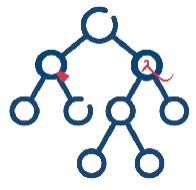
\includegraphics[height=1.0cm]{msca_logo.png}}%
    \end{center}

    \vspace{0.6cm}

    % Main title with Q logos on sides (with clickable links)
    \begin{center}
        \begin{minipage}{0.1\textwidth}
            \centering
            \href{https://quantlet.com}{
\includegraphics[height=1.1cm]{ql_logo.png}}
        \end{minipage}%
        \begin{minipage}{0.78\textwidth}
            \centering
            {\LARGE\bfseries\usebeamercolor[fg]{title}\inserttitle}

            \vspace{0.3cm}

            {\usebeamerfont{subtitle}\usebeamercolor[fg]{title}\insertsubtitle}
        \end{minipage}%
        \begin{minipage}{0.1\textwidth}
            \centering
            \href{https://quantinar.com}{
\includegraphics[height=1.1cm]{qr_logo.png}}
        \end{minipage}
    \end{center}

    \vspace{0.6cm}

    % Authors (left aligned)
    \hspace{0.5cm}{\usebeamerfont{author}\insertauthor}

    \vspace{0.3cm}

    % Institute/Affiliations (left aligned)
    \hspace{0.5cm}\begin{minipage}[t]{0.9\textwidth}
        \raggedright\small\insertinstitute
    \end{minipage}
}

%=============================================================================
% THEOREM ENVIRONMENTS
%=============================================================================
\theoremstyle{definition}
\setbeamertemplate{theorems}[numbered]
\ifdefined\sfmlang
\newtheorem{defn}{Definiție}
\newtheorem{thm}{Teoremă}
\newtheorem{prop}{Propoziție}
\newtheorem{rmk}{Observație}
\else
\newtheorem{defn}{Definition}
\newtheorem{thm}{Theorem}
\newtheorem{prop}{Proposition}
\newtheorem{rmk}{Remark}
\fi

%=============================================================================
% CENTRED MINIPAGE (no extra vertical space)
%=============================================================================
\newenvironment{cminipage}[1]{%
    \par\noindent\hfill\begin{minipage}{#1}\ignorespaces
}{%
    \end{minipage}\hfill\null\par
}

%=============================================================================
% CUSTOM COMMANDS
%=============================================================================
\newcommand{\E}{\mathbb{E}}
\newcommand{\Var}{\text{Var}}
\newcommand{\Cov}{\text{Cov}}
\newcommand{\Corr}{\text{Corr}}
\newcommand{\R}{\mathbb{R}}
\newcommand{\N}{\mathbb{N}}
\newcommand{\Z}{\mathbb{Z}}
\newcommand{\B}{\mathbf{B}}
\newcommand{\imark}{\textcolor{MainBlue}{\textbullet}}
\newcommand{\RMSE}{\text{RMSE}}
\newcommand{\MAE}{\text{MAE}}
\newcommand{\MAPE}{\text{MAPE}}

 se definește
%   \newcommand{\coursename}{Statistics of Financial Markets}      (EN)
%   \newcommand{\coursename}{Statistica piețelor financiare}       (RO)  și  \def\sfmlang{ro}
% Fișierele .tex se află în EN/Courses, EN/Seminars, RO/Cursuri, RO/Seminarii (două niveluri sub rădăcină).
% Deck-urile sînt generate de latex/build_chapterN.py / build_seminarN.py (vezi latex/sfm_build.py).

\documentclass[9pt, aspectratio=169, t]{beamer}
\providecommand{\coursename}{Statistics of Financial Markets}

% Ensure content fits on slides
\setbeamersize{text margin left=8mm, text margin right=8mm}

%=============================================================================
% THEME AND STYLE CONFIGURATION
%=============================================================================
\usetheme{default}
% Using default theme for clean header/footer control

% Color Palette (matching Redispatch PDF)
\definecolor{MainBlue}{RGB}{26, 58, 110}
\definecolor{AccentBlue}{RGB}{26, 58, 110}
\definecolor{IDAred}{RGB}{205, 0, 0}
\definecolor{DarkGray}{RGB}{51, 51, 51}
\definecolor{MediumGray}{RGB}{128, 128, 128}
\definecolor{LightGray}{RGB}{248, 248, 248}
\definecolor{VeryLightGray}{RGB}{235, 235, 235}
\definecolor{KeynoteGray}{RGB}{218, 218, 218}
\definecolor{SectionGray}{RGB}{120, 120, 120}
\definecolor{FooterGray}{RGB}{100, 100, 100}
\definecolor{Crimson}{RGB}{220, 53, 69}
\definecolor{Forest}{RGB}{46, 125, 50}
\definecolor{Amber}{RGB}{181, 133, 63}
\definecolor{Orange}{RGB}{230, 126, 34}
\definecolor{Purple}{RGB}{142, 68, 173}

% Gradient background (exact Keynote 315° gradient: white to RGB 218,218,218)
\setbeamertemplate{background}{%
    \begin{tikzpicture}[remember picture, overlay]
        \shade[shading=axis, shading angle=315,
        top color=white, bottom color=KeynoteGray]
        (current page.south west) rectangle (current page.north east);
    \end{tikzpicture}%
}
% Fallback solid color for compatibility
\setbeamercolor{background canvas}{bg=}

\setbeamercolor{palette primary}{bg=MainBlue, fg=white}
\setbeamercolor{palette secondary}{bg=MainBlue!85, fg=white}
\setbeamercolor{palette tertiary}{bg=MainBlue!70, fg=white}
\setbeamercolor{structure}{fg=MainBlue}
\setbeamercolor{title}{fg=IDAred}
\setbeamercolor{frametitle}{fg=IDAred, bg=}
\setbeamercolor{block title}{bg=MainBlue, fg=white}
\setbeamercolor{block body}{bg=VeryLightGray, fg=DarkGray}
\setbeamercolor{block title alerted}{bg=Crimson, fg=white}
\setbeamercolor{block body alerted}{bg=Crimson!8, fg=DarkGray}
\setbeamercolor{block title example}{bg=Forest, fg=white}
\setbeamercolor{block body example}{bg=Forest!8, fg=DarkGray}
\setbeamercolor{item}{fg=MainBlue}

% Footer colors (override Madrid theme blue)
\setbeamercolor{author in head/foot}{fg=FooterGray, bg=}
\setbeamercolor{title in head/foot}{fg=FooterGray, bg=}
\setbeamercolor{date in head/foot}{fg=FooterGray, bg=}
\setbeamercolor{section in head/foot}{fg=FooterGray, bg=}
\setbeamercolor{subsection in head/foot}{fg=FooterGray, bg=}

% Bullet styles (apply everywhere including blocks)
\setbeamertemplate{itemize item}{\color{MainBlue}$\boxdot$}
\setbeamertemplate{itemize subitem}{\color{MainBlue}$\blacktriangleright$}
\setbeamertemplate{itemize subsubitem}{\color{MainBlue}\tiny$\bullet$}
\setbeamertemplate{itemize/enumerate body begin}{\normalsize}
\setbeamertemplate{itemize/enumerate subbody begin}{\normalsize}

% Item spacing - compact style
\setlength{\leftmargini}{10pt}       % Level 1: minimal indent
\setlength{\leftmarginii}{10pt}      % Level 2: minimal additional indent
% Compact list spacing (zero extra space before/after lists in blocks)
\makeatletter
\def\@listi{\leftmargin\leftmargini \topsep 0pt \parsep 0pt \itemsep 0pt}
\def\@listii{\leftmargin\leftmarginii \topsep 0pt \parsep 0pt \itemsep 0pt}
\makeatother

\setbeamertemplate{navigation symbols}{}

%=============================================================================
% CUSTOM HEADLINE
%=============================================================================
\setbeamertemplate{headline}{%
    \vskip10pt%
    \hbox to \paperwidth{%
        \hskip0.5cm%
        {\small\color{FooterGray}\renewcommand{\hyperlink}[2]{##2}\insertsectionhead}%
        \hfill%
        \textcolor{FooterGray}{\small\insertframenumber}%
        \hskip0.5cm%
    }%
    \vskip4pt%
    {\color{FooterGray}\hrule height 0.4pt}%
}

%=============================================================================
% CUSTOM FOOTER
%=============================================================================
\usepackage{fontawesome5}

\setbeamertemplate{footline}{%
    {\color{FooterGray}\hrule height 0.4pt}%
    \vskip4pt%
    \hbox to \paperwidth{%
        \hskip0.5cm%
        \textcolor{FooterGray}{\small\coursename}%
        \hfill%
        \raisebox{-0.1em}{%
            \begin{tikzpicture}[x=0.08em, y=0.08em, line width=0.4pt]
                \draw[FooterGray] (0,3) -- (1,4) -- (2,3.5) -- (3,5) -- (4,4) -- (5,6) -- (6,5.5) -- (7,4) -- (8,5) -- (9,7) -- (10,6) -- (11,5) -- (12,6.5) -- (13,8) -- (14,7) -- (15,6) -- (16,7.5) -- (17,9) -- (18,8) -- (19,7) -- (20,8.5) -- (21,10) -- (22,9) -- (23,8) -- (24,9.5);
            \end{tikzpicture}%
        }%
        \hskip0.5cm%
    }%
    \vskip6pt%
}

%=============================================================================
% PACKAGES
%=============================================================================
\usepackage[utf8]{inputenc}
\DeclareUnicodeCharacter{03B1}{\ensuremath{\alpha}}
\usepackage[T1]{fontenc}
\usepackage{amsmath, amssymb, amsthm}
\usepackage{mathtools}
\usepackage{bm}
\usepackage{tikz}
\usetikzlibrary{arrows.meta, positioning, shapes, calc, decorations.pathreplacing, shadings}
\usepackage{booktabs}
\usepackage{multirow}
\usepackage{array}
\usepackage{graphicx}
\usepackage{hyperref}
\usepackage{colortbl}
\usepackage{listings}
\lstset{language=Python, basicstyle=\ttfamily\scriptsize, keywordstyle=\color{MainBlue}\bfseries,
  commentstyle=\color{Forest}, stringstyle=\color{Crimson}, breaklines=true,
  frame=none, backgroundcolor=\color{VeryLightGray}, xleftmargin=2mm}
\hypersetup{colorlinks=true, linkcolor=MainBlue, urlcolor=MainBlue}
\graphicspath{{../../logos/}{../../charts/}{../../photos/}}
\usepackage{xcolor}
\hfuzz=2pt  % Suppress tiny overfull warnings (<2pt)
\vfuzz=2pt  % Suppress tiny vertical overfull warnings (<2pt)

%=============================================================================
% QUANTLET COMMANDS
%   \quantlet{<displayed name>}{<url>}       (generic, compatible with the older SFM decks)
%   \sfmquantlet{Ch_05}{SFM_ch5_garch}       -> https://github.com/danpele/SFM/tree/main/Quantlets/Ch_05/SFM_ch5_garch
%   \qlurl{<folder>} is defined per chapter by the generator (Quantlets/Ch_NN/<folder>)
%=============================================================================
\newcommand{\sfmrepo}{https://github.com/danpele/SFM}
\newcommand{\sfmqlbase}{https://github.com/danpele/SFM/tree/main/Quantlets}
\newcommand{\quantlet}[2]{%
    \hfill\href{#2}{%
        \raisebox{-0.15em}{
\includegraphics[height=0.7em]{ql_logo.png}}%
        \textcolor{MainBlue}{\tiny\ #1}%
    }%
}
\newcommand{\sfmquantlet}[2]{\quantlet{\detokenize{#2}}{\sfmqlbase/#1/#2}}

%=============================================================================
% NOTEBOOKS (Google Colab)
%   \colaburl{notebooks/EN/chapter5_seminar_notebook.ipynb} -> the Colab link of a file in the SFM repo
%   \nb: the chapter notebook (each seminar deck redefines it with \renewcommand)
%=============================================================================
\newcommand{\colaburl}[1]{https://colab.research.google.com/github/danpele/SFM/blob/main/#1}
\newcommand{\nb}{https://colab.research.google.com/github/danpele/SFM/tree/main/notebooks/EN}
\newcommand{\nbname}{notebooks/EN}

%=============================================================================
% SLIDE HELPERS (used by the generators; the same as in MFM)
%=============================================================================
% local font size for list bodies (the preamble forces \normalsize)
\newcommand{\itemsize}[1]{\setbeamertemplate{itemize/enumerate body begin}{#1}\setbeamertemplate{itemize/enumerate subbody begin}{#1}}
\newcommand{\intitle}[1]{{\hypersetup{urlcolor=white}#1}}   % white links inside coloured title bars
\newcommand{\imgcap}[1]{{\scriptsize #1}\\[0.5mm]}          % caption under a photo
\newcommand{\imgcredit}[2]{{\tiny\color{FooterGray}\href{#1}{#2}}}   % image credit: source URL, author/licence
\newcommand{\aiprompt}[1]{{\ttfamily\color{MainBlue}#1}}     % a prompt to an AI assistant

%=============================================================================
% SEMINARS: student version by default; the instructor wrapper *_solutions.tex sets \solutionstrue
%=============================================================================
\makeatletter\@ifundefined{ifsolutions}{\expandafter\newif\csname ifsolutions\endcsname}{}\makeatother
\newcommand{\solonly}[1]{\ifsolutions #1\fi}
\newcommand{\propsub}{\ifsolutions\else\framesubtitle{\ifdefined\sfmlang Rezolvarea se discută la seminar\else Solution discussed in class\fi}\fi}

%=============================================================================
% APPENDIX AND CHAPTER LINKS (latex/appendix_links.py writes the calls; it also re-declares these
% macros before \begin{document}, so the decks compile with or without this preamble block)
%=============================================================================
\providecommand{\sfmapplink}[3]{\hypertarget{#2}{}\hyperlink{#1}{\beamergotobutton{#3}}}
\providecommand{\sfmappback}[2]{\begin{tikzpicture}[remember picture,overlay]\node[anchor=south east] at ([xshift=-3mm,yshift=7mm]current page.south east){\hyperlink{#1}{\beamerreturnbutton{#2}}};\end{tikzpicture}}
\providecommand{\sfmchlink}[2]{\href{#1}{#2}}
\providecommand{\sfmchlinkt}[2]{\href{#1}{\usebeamercolor[fg]{frametitle}#2}}

%=============================================================================
% QUANTINAR COMMAND: link către un curs Quantinar (subiecte avansate)
%=============================================================================
\newcommand{\quantinar}[2]{%
    \href{#2}{%
        \raisebox{-0.15em}{
\includegraphics[height=0.8em]{qr_logo.png}}%
        \textcolor{MainBlue}{\scriptsize\ #1}%
    }%
}

%=============================================================================
% CUSTOM TITLE PAGE
%=============================================================================
\defbeamertemplate*{title page}{hybrid}[1][]
{
    \vspace{0.2cm}
    % Logos row - top header (with clickable links)
    \begin{center}
        \href{https://www.ase.ro}{
\includegraphics[height=1.0cm]{ase_logo.png}}\hspace{0.3cm}%
        \href{https://theida.net}{
\includegraphics[height=1.0cm]{ida_logo.png}}\hspace{0.3cm}%
        \href{https://blockchain-research-center.com}{
\includegraphics[height=1.0cm]{brc_logo.png}}\hspace{0.3cm}%
        \href{https://www.ai4efin.ase.ro}{
\includegraphics[height=1.0cm]{ai4efin_logo.png}}\hspace{0.3cm}%
        \href{https://ipe.ro/new}{
\includegraphics[height=1.0cm]{acad_logo.png}}\hspace{0.3cm}%
        \href{https://www.digital-finance-msca.com}{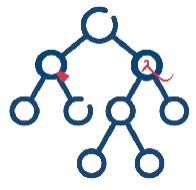
\includegraphics[height=1.0cm]{msca_logo.png}}%
    \end{center}

    \vspace{0.6cm}

    % Main title with Q logos on sides (with clickable links)
    \begin{center}
        \begin{minipage}{0.1\textwidth}
            \centering
            \href{https://quantlet.com}{
\includegraphics[height=1.1cm]{ql_logo.png}}
        \end{minipage}%
        \begin{minipage}{0.78\textwidth}
            \centering
            {\LARGE\bfseries\usebeamercolor[fg]{title}\inserttitle}

            \vspace{0.3cm}

            {\usebeamerfont{subtitle}\usebeamercolor[fg]{title}\insertsubtitle}
        \end{minipage}%
        \begin{minipage}{0.1\textwidth}
            \centering
            \href{https://quantinar.com}{
\includegraphics[height=1.1cm]{qr_logo.png}}
        \end{minipage}
    \end{center}

    \vspace{0.6cm}

    % Authors (left aligned)
    \hspace{0.5cm}{\usebeamerfont{author}\insertauthor}

    \vspace{0.3cm}

    % Institute/Affiliations (left aligned)
    \hspace{0.5cm}\begin{minipage}[t]{0.9\textwidth}
        \raggedright\small\insertinstitute
    \end{minipage}
}

%=============================================================================
% THEOREM ENVIRONMENTS
%=============================================================================
\theoremstyle{definition}
\setbeamertemplate{theorems}[numbered]
\ifdefined\sfmlang
\newtheorem{defn}{Definiție}
\newtheorem{thm}{Teoremă}
\newtheorem{prop}{Propoziție}
\newtheorem{rmk}{Observație}
\else
\newtheorem{defn}{Definition}
\newtheorem{thm}{Theorem}
\newtheorem{prop}{Proposition}
\newtheorem{rmk}{Remark}
\fi

%=============================================================================
% CENTRED MINIPAGE (no extra vertical space)
%=============================================================================
\newenvironment{cminipage}[1]{%
    \par\noindent\hfill\begin{minipage}{#1}\ignorespaces
}{%
    \end{minipage}\hfill\null\par
}

%=============================================================================
% CUSTOM COMMANDS
%=============================================================================
\newcommand{\E}{\mathbb{E}}
\newcommand{\Var}{\text{Var}}
\newcommand{\Cov}{\text{Cov}}
\newcommand{\Corr}{\text{Corr}}
\newcommand{\R}{\mathbb{R}}
\newcommand{\N}{\mathbb{N}}
\newcommand{\Z}{\mathbb{Z}}
\newcommand{\B}{\mathbf{B}}
\newcommand{\imark}{\textcolor{MainBlue}{\textbullet}}
\newcommand{\RMSE}{\text{RMSE}}
\newcommand{\MAE}{\text{MAE}}
\newcommand{\MAPE}{\text{MAPE}}

 se definește
%   \newcommand{\coursename}{Statistics of Financial Markets}      (EN)
%   \newcommand{\coursename}{Statistica piețelor financiare}       (RO)  și  \def\sfmlang{ro}
% Fișierele .tex se află în EN/Courses, EN/Seminars, RO/Cursuri, RO/Seminarii (două niveluri sub rădăcină).
% Deck-urile sînt generate de latex/build_chapterN.py / build_seminarN.py (vezi latex/sfm_build.py).

\documentclass[9pt, aspectratio=169, t]{beamer}
\providecommand{\coursename}{Statistics of Financial Markets}

% Ensure content fits on slides
\setbeamersize{text margin left=8mm, text margin right=8mm}

%=============================================================================
% THEME AND STYLE CONFIGURATION
%=============================================================================
\usetheme{default}
% Using default theme for clean header/footer control

% Color Palette (matching Redispatch PDF)
\definecolor{MainBlue}{RGB}{26, 58, 110}
\definecolor{AccentBlue}{RGB}{26, 58, 110}
\definecolor{IDAred}{RGB}{205, 0, 0}
\definecolor{DarkGray}{RGB}{51, 51, 51}
\definecolor{MediumGray}{RGB}{128, 128, 128}
\definecolor{LightGray}{RGB}{248, 248, 248}
\definecolor{VeryLightGray}{RGB}{235, 235, 235}
\definecolor{KeynoteGray}{RGB}{218, 218, 218}
\definecolor{SectionGray}{RGB}{120, 120, 120}
\definecolor{FooterGray}{RGB}{100, 100, 100}
\definecolor{Crimson}{RGB}{220, 53, 69}
\definecolor{Forest}{RGB}{46, 125, 50}
\definecolor{Amber}{RGB}{181, 133, 63}
\definecolor{Orange}{RGB}{230, 126, 34}
\definecolor{Purple}{RGB}{142, 68, 173}

% Gradient background (exact Keynote 315° gradient: white to RGB 218,218,218)
\setbeamertemplate{background}{%
    \begin{tikzpicture}[remember picture, overlay]
        \shade[shading=axis, shading angle=315,
        top color=white, bottom color=KeynoteGray]
        (current page.south west) rectangle (current page.north east);
    \end{tikzpicture}%
}
% Fallback solid color for compatibility
\setbeamercolor{background canvas}{bg=}

\setbeamercolor{palette primary}{bg=MainBlue, fg=white}
\setbeamercolor{palette secondary}{bg=MainBlue!85, fg=white}
\setbeamercolor{palette tertiary}{bg=MainBlue!70, fg=white}
\setbeamercolor{structure}{fg=MainBlue}
\setbeamercolor{title}{fg=IDAred}
\setbeamercolor{frametitle}{fg=IDAred, bg=}
\setbeamercolor{block title}{bg=MainBlue, fg=white}
\setbeamercolor{block body}{bg=VeryLightGray, fg=DarkGray}
\setbeamercolor{block title alerted}{bg=Crimson, fg=white}
\setbeamercolor{block body alerted}{bg=Crimson!8, fg=DarkGray}
\setbeamercolor{block title example}{bg=Forest, fg=white}
\setbeamercolor{block body example}{bg=Forest!8, fg=DarkGray}
\setbeamercolor{item}{fg=MainBlue}

% Footer colors (override Madrid theme blue)
\setbeamercolor{author in head/foot}{fg=FooterGray, bg=}
\setbeamercolor{title in head/foot}{fg=FooterGray, bg=}
\setbeamercolor{date in head/foot}{fg=FooterGray, bg=}
\setbeamercolor{section in head/foot}{fg=FooterGray, bg=}
\setbeamercolor{subsection in head/foot}{fg=FooterGray, bg=}

% Bullet styles (apply everywhere including blocks)
\setbeamertemplate{itemize item}{\color{MainBlue}$\boxdot$}
\setbeamertemplate{itemize subitem}{\color{MainBlue}$\blacktriangleright$}
\setbeamertemplate{itemize subsubitem}{\color{MainBlue}\tiny$\bullet$}
\setbeamertemplate{itemize/enumerate body begin}{\normalsize}
\setbeamertemplate{itemize/enumerate subbody begin}{\normalsize}

% Item spacing - compact style
\setlength{\leftmargini}{10pt}       % Level 1: minimal indent
\setlength{\leftmarginii}{10pt}      % Level 2: minimal additional indent
% Compact list spacing (zero extra space before/after lists in blocks)
\makeatletter
\def\@listi{\leftmargin\leftmargini \topsep 0pt \parsep 0pt \itemsep 0pt}
\def\@listii{\leftmargin\leftmarginii \topsep 0pt \parsep 0pt \itemsep 0pt}
\makeatother

\setbeamertemplate{navigation symbols}{}

%=============================================================================
% CUSTOM HEADLINE
%=============================================================================
\setbeamertemplate{headline}{%
    \vskip10pt%
    \hbox to \paperwidth{%
        \hskip0.5cm%
        {\small\color{FooterGray}\renewcommand{\hyperlink}[2]{##2}\insertsectionhead}%
        \hfill%
        \textcolor{FooterGray}{\small\insertframenumber}%
        \hskip0.5cm%
    }%
    \vskip4pt%
    {\color{FooterGray}\hrule height 0.4pt}%
}

%=============================================================================
% CUSTOM FOOTER
%=============================================================================
\usepackage{fontawesome5}

\setbeamertemplate{footline}{%
    {\color{FooterGray}\hrule height 0.4pt}%
    \vskip4pt%
    \hbox to \paperwidth{%
        \hskip0.5cm%
        \textcolor{FooterGray}{\small\coursename}%
        \hfill%
        \raisebox{-0.1em}{%
            \begin{tikzpicture}[x=0.08em, y=0.08em, line width=0.4pt]
                \draw[FooterGray] (0,3) -- (1,4) -- (2,3.5) -- (3,5) -- (4,4) -- (5,6) -- (6,5.5) -- (7,4) -- (8,5) -- (9,7) -- (10,6) -- (11,5) -- (12,6.5) -- (13,8) -- (14,7) -- (15,6) -- (16,7.5) -- (17,9) -- (18,8) -- (19,7) -- (20,8.5) -- (21,10) -- (22,9) -- (23,8) -- (24,9.5);
            \end{tikzpicture}%
        }%
        \hskip0.5cm%
    }%
    \vskip6pt%
}

%=============================================================================
% PACKAGES
%=============================================================================
\usepackage[utf8]{inputenc}
\DeclareUnicodeCharacter{03B1}{\ensuremath{\alpha}}
\usepackage[T1]{fontenc}
\usepackage{amsmath, amssymb, amsthm}
\usepackage{mathtools}
\usepackage{bm}
\usepackage{tikz}
\usetikzlibrary{arrows.meta, positioning, shapes, calc, decorations.pathreplacing, shadings}
\usepackage{booktabs}
\usepackage{multirow}
\usepackage{array}
\usepackage{graphicx}
\usepackage{hyperref}
\usepackage{colortbl}
\usepackage{listings}
\lstset{language=Python, basicstyle=\ttfamily\scriptsize, keywordstyle=\color{MainBlue}\bfseries,
  commentstyle=\color{Forest}, stringstyle=\color{Crimson}, breaklines=true,
  frame=none, backgroundcolor=\color{VeryLightGray}, xleftmargin=2mm}
\hypersetup{colorlinks=true, linkcolor=MainBlue, urlcolor=MainBlue}
\graphicspath{{../../logos/}{../../charts/}{../../photos/}}
\usepackage{xcolor}
\hfuzz=2pt  % Suppress tiny overfull warnings (<2pt)
\vfuzz=2pt  % Suppress tiny vertical overfull warnings (<2pt)

%=============================================================================
% QUANTLET COMMANDS
%   \quantlet{<displayed name>}{<url>}       (generic, compatible with the older SFM decks)
%   \sfmquantlet{Ch_05}{SFM_ch5_garch}       -> https://github.com/danpele/SFM/tree/main/Quantlets/Ch_05/SFM_ch5_garch
%   \qlurl{<folder>} is defined per chapter by the generator (Quantlets/Ch_NN/<folder>)
%=============================================================================
\newcommand{\sfmrepo}{https://github.com/danpele/SFM}
\newcommand{\sfmqlbase}{https://github.com/danpele/SFM/tree/main/Quantlets}
\newcommand{\quantlet}[2]{%
    \hfill\href{#2}{%
        \raisebox{-0.15em}{
\includegraphics[height=0.7em]{ql_logo.png}}%
        \textcolor{MainBlue}{\tiny\ #1}%
    }%
}
\newcommand{\sfmquantlet}[2]{\quantlet{\detokenize{#2}}{\sfmqlbase/#1/#2}}

%=============================================================================
% NOTEBOOKS (Google Colab)
%   \colaburl{notebooks/EN/chapter5_seminar_notebook.ipynb} -> the Colab link of a file in the SFM repo
%   \nb: the chapter notebook (each seminar deck redefines it with \renewcommand)
%=============================================================================
\newcommand{\colaburl}[1]{https://colab.research.google.com/github/danpele/SFM/blob/main/#1}
\newcommand{\nb}{https://colab.research.google.com/github/danpele/SFM/tree/main/notebooks/EN}
\newcommand{\nbname}{notebooks/EN}

%=============================================================================
% SLIDE HELPERS (used by the generators; the same as in MFM)
%=============================================================================
% local font size for list bodies (the preamble forces \normalsize)
\newcommand{\itemsize}[1]{\setbeamertemplate{itemize/enumerate body begin}{#1}\setbeamertemplate{itemize/enumerate subbody begin}{#1}}
\newcommand{\intitle}[1]{{\hypersetup{urlcolor=white}#1}}   % white links inside coloured title bars
\newcommand{\imgcap}[1]{{\scriptsize #1}\\[0.5mm]}          % caption under a photo
\newcommand{\imgcredit}[2]{{\tiny\color{FooterGray}\href{#1}{#2}}}   % image credit: source URL, author/licence
\newcommand{\aiprompt}[1]{{\ttfamily\color{MainBlue}#1}}     % a prompt to an AI assistant

%=============================================================================
% SEMINARS: student version by default; the instructor wrapper *_solutions.tex sets \solutionstrue
%=============================================================================
\makeatletter\@ifundefined{ifsolutions}{\expandafter\newif\csname ifsolutions\endcsname}{}\makeatother
\newcommand{\solonly}[1]{\ifsolutions #1\fi}
\newcommand{\propsub}{\ifsolutions\else\framesubtitle{\ifdefined\sfmlang Rezolvarea se discută la seminar\else Solution discussed in class\fi}\fi}

%=============================================================================
% APPENDIX AND CHAPTER LINKS (latex/appendix_links.py writes the calls; it also re-declares these
% macros before \begin{document}, so the decks compile with or without this preamble block)
%=============================================================================
\providecommand{\sfmapplink}[3]{\hypertarget{#2}{}\hyperlink{#1}{\beamergotobutton{#3}}}
\providecommand{\sfmappback}[2]{\begin{tikzpicture}[remember picture,overlay]\node[anchor=south east] at ([xshift=-3mm,yshift=7mm]current page.south east){\hyperlink{#1}{\beamerreturnbutton{#2}}};\end{tikzpicture}}
\providecommand{\sfmchlink}[2]{\href{#1}{#2}}
\providecommand{\sfmchlinkt}[2]{\href{#1}{\usebeamercolor[fg]{frametitle}#2}}

%=============================================================================
% QUANTINAR COMMAND: link către un curs Quantinar (subiecte avansate)
%=============================================================================
\newcommand{\quantinar}[2]{%
    \href{#2}{%
        \raisebox{-0.15em}{
\includegraphics[height=0.8em]{qr_logo.png}}%
        \textcolor{MainBlue}{\scriptsize\ #1}%
    }%
}

%=============================================================================
% CUSTOM TITLE PAGE
%=============================================================================
\defbeamertemplate*{title page}{hybrid}[1][]
{
    \vspace{0.2cm}
    % Logos row - top header (with clickable links)
    \begin{center}
        \href{https://www.ase.ro}{
\includegraphics[height=1.0cm]{ase_logo.png}}\hspace{0.3cm}%
        \href{https://theida.net}{
\includegraphics[height=1.0cm]{ida_logo.png}}\hspace{0.3cm}%
        \href{https://blockchain-research-center.com}{
\includegraphics[height=1.0cm]{brc_logo.png}}\hspace{0.3cm}%
        \href{https://www.ai4efin.ase.ro}{
\includegraphics[height=1.0cm]{ai4efin_logo.png}}\hspace{0.3cm}%
        \href{https://ipe.ro/new}{
\includegraphics[height=1.0cm]{acad_logo.png}}\hspace{0.3cm}%
        \href{https://www.digital-finance-msca.com}{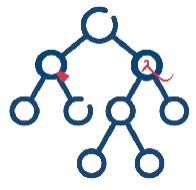
\includegraphics[height=1.0cm]{msca_logo.png}}%
    \end{center}

    \vspace{0.6cm}

    % Main title with Q logos on sides (with clickable links)
    \begin{center}
        \begin{minipage}{0.1\textwidth}
            \centering
            \href{https://quantlet.com}{
\includegraphics[height=1.1cm]{ql_logo.png}}
        \end{minipage}%
        \begin{minipage}{0.78\textwidth}
            \centering
            {\LARGE\bfseries\usebeamercolor[fg]{title}\inserttitle}

            \vspace{0.3cm}

            {\usebeamerfont{subtitle}\usebeamercolor[fg]{title}\insertsubtitle}
        \end{minipage}%
        \begin{minipage}{0.1\textwidth}
            \centering
            \href{https://quantinar.com}{
\includegraphics[height=1.1cm]{qr_logo.png}}
        \end{minipage}
    \end{center}

    \vspace{0.6cm}

    % Authors (left aligned)
    \hspace{0.5cm}{\usebeamerfont{author}\insertauthor}

    \vspace{0.3cm}

    % Institute/Affiliations (left aligned)
    \hspace{0.5cm}\begin{minipage}[t]{0.9\textwidth}
        \raggedright\small\insertinstitute
    \end{minipage}
}

%=============================================================================
% THEOREM ENVIRONMENTS
%=============================================================================
\theoremstyle{definition}
\setbeamertemplate{theorems}[numbered]
\ifdefined\sfmlang
\newtheorem{defn}{Definiție}
\newtheorem{thm}{Teoremă}
\newtheorem{prop}{Propoziție}
\newtheorem{rmk}{Observație}
\else
\newtheorem{defn}{Definition}
\newtheorem{thm}{Theorem}
\newtheorem{prop}{Proposition}
\newtheorem{rmk}{Remark}
\fi

%=============================================================================
% CENTRED MINIPAGE (no extra vertical space)
%=============================================================================
\newenvironment{cminipage}[1]{%
    \par\noindent\hfill\begin{minipage}{#1}\ignorespaces
}{%
    \end{minipage}\hfill\null\par
}

%=============================================================================
% CUSTOM COMMANDS
%=============================================================================
\newcommand{\E}{\mathbb{E}}
\newcommand{\Var}{\text{Var}}
\newcommand{\Cov}{\text{Cov}}
\newcommand{\Corr}{\text{Corr}}
\newcommand{\R}{\mathbb{R}}
\newcommand{\N}{\mathbb{N}}
\newcommand{\Z}{\mathbb{Z}}
\newcommand{\B}{\mathbf{B}}
\newcommand{\imark}{\textcolor{MainBlue}{\textbullet}}
\newcommand{\RMSE}{\text{RMSE}}
\newcommand{\MAE}{\text{MAE}}
\newcommand{\MAPE}{\text{MAPE}}



\newcommand{\qlurl}[1]{https://github.com/danpele/SFM/tree/main/Quantlets/Ch_13/#1}

% Clickable citations (DOIs verified via Crossref)

\newcommand{\refFHH}{\href{https://doi.org/10.1007/978-3-030-13751-9}{Franke, Härdle \& Hafner (2019)}}
\newcommand{\refBHL}{\href{https://doi.org/10.1007/978-3-642-33929-5}{Borak, Härdle \& López-Cabrera (2013)}}
\newcommand{\refISL}{\href{https://doi.org/10.1007/978-3-031-38747-0}{James et al.\ (2023)}}
\newcommand{\refHTF}{\href{https://doi.org/10.1007/978-0-387-84858-7}{Hastie, Tibshirani \& Friedman (2009)}}
\newcommand{\refBreimanTC}{\href{https://doi.org/10.1214/ss/1009213726}{Breiman (2001a)}}
\newcommand{\refBreiman}{\href{https://doi.org/10.1023/A:1010933404324}{Breiman (2001b)}}
\newcommand{\refFriedman}{\href{https://doi.org/10.1214/aos/1013203451}{Friedman (2001)}}
\newcommand{\refHK}{\href{https://doi.org/10.1080/00401706.1970.10488634}{Hoerl \& Kennard (1970)}}
\newcommand{\refTib}{\href{https://doi.org/10.1111/j.2517-6161.1996.tb02080.x}{Tibshirani (1996)}}
\newcommand{\refRosenblatt}{\href{https://doi.org/10.1037/h0042519}{Rosenblatt (1958)}}
\newcommand{\refHSW}{\href{https://doi.org/10.1016/0893-6080(89)90020-8}{Hornik, Stinchcombe \& White (1989)}}
\newcommand{\refRHW}{\href{https://doi.org/10.1038/323533a0}{Rumelhart, Hinton \& Williams (1986)}}
\newcommand{\refCorsi}{\href{https://doi.org/10.1093/jjfinec/nbp001}{Corsi (2009)}}
\newcommand{\refGK}{\href{https://doi.org/10.1086/296072}{Garman \& Klass (1980)}}
\newcommand{\refPatton}{\href{https://doi.org/10.1016/j.jeconom.2010.03.034}{Patton (2011)}}
\newcommand{\refDM}{\href{https://doi.org/10.1080/07350015.1995.10524599}{Diebold \& Mariano (1995)}}
\newcommand{\refCT}{\href{https://doi.org/10.1093/rfs/hhm055}{Campbell \& Thompson (2008)}}
\newcommand{\refWG}{\href{https://doi.org/10.1093/rfs/hhm014}{Welch \& Goyal (2008)}}
\newcommand{\refKB}{\href{https://doi.org/10.2307/1913643}{Koenker \& Bassett (1978)}}
\newcommand{\refCAViaR}{\href{https://doi.org/10.1198/073500104000000370}{Engle \& Manganelli (2004)}}
\newcommand{\refKupiec}{\href{https://doi.org/10.3905/jod.1995.407942}{Kupiec (1995)}}
\newcommand{\refChris}{\href{https://doi.org/10.2307/2527341}{Christoffersen (1998)}}
\newcommand{\refBLdP}{\href{https://doi.org/10.3905/jpm.2014.40.5.094}{Bailey \& López de Prado (2014)}}
\newcommand{\refHLZ}{\href{https://doi.org/10.1093/rfs/hhv059}{Harvey, Liu \& Zhu (2016)}}
\newcommand{\refWhite}{\href{https://doi.org/10.1111/1468-0262.00152}{White (2000)}}
\newcommand{\refLdP}{\href{https://www.wiley.com/en-us/Advances+in+Financial+Machine+Learning-p-9781119482086}{López de Prado (2018)}}
\newcommand{\refBHK}{\href{https://doi.org/10.1016/j.csda.2017.11.003}{Bergmeir, Hyndman \& Koo (2018)}}
\newcommand{\refGKX}{\href{https://doi.org/10.1093/rfs/hhaa009}{Gu, Kelly \& Xiu (2020)}}
\newcommand{\refKX}{\href{https://doi.org/10.1561/0500000064}{Kelly \& Xiu (2023)}}
\newcommand{\refCSV}{\href{https://doi.org/10.1093/jjfinec/nbac020}{Christensen, Siggaard \& Veliyev (2023)}}
\newcommand{\refLL}{\href{https://proceedings.neurips.cc/paper/2017/hash/8a20a8621978632d76c43dfd28b67767-Abstract.html}{Lundberg \& Lee (2017)}}
\newcommand{\refEngle}{\href{https://doi.org/10.2307/1912773}{Engle (1982)}}
\newcommand{\refBoll}{\href{https://doi.org/10.1016/0304-4076(86)90063-1}{Bollerslev (1986)}}
\newcommand{\refWang}{\href{https://doi.org/10.1038/s41586-023-06221-2}{Wang et al.\ (2023)}}
\newcommand{\refPeleA}{\href{https://doi.org/10.1080/1351847X.2021.1960403}{Pele et al.\ (2023)}}
\newcommand{\refPeleB}{\href{https://doi.org/10.3390/math14132316}{Pele \& Mazurencu-Marinescu-Pele (2026)}}
\newcommand{\refSFEa}{\href{https://github.com/QuantLet/SFE/tree/master/QID-3386-SFEnnarch}{SFEnnarch}}
\newcommand{\refSFEb}{\href{https://github.com/QuantLet/SFE/tree/master/QID-3387-SFEnnjpyusd}{SFEnnjpyusd}}

\title[Statistics of Financial Markets]{Statistics of Financial Markets}
\subtitle{Chapter 13: Machine learning}
\author[D.T. Pele]{Daniel Traian PELE}
\institute{Bucharest University of Economic Studies\\
IDA Institute Digital Assets\\
Blockchain Research Center\\
AI4EFin Artificial Intelligence for Energy Finance\\
Romanian Academy, Institute for Economic Forecasting\\
MSCA Digital Finance}
\date{}

%=============================================================================
\providecommand{\sfmapplink}[3]{\hypertarget{#2}{}\hyperlink{#1}{\beamergotobutton{#3}}}  % APPLINKS-MACROS
\providecommand{\sfmappback}[2]{\begin{tikzpicture}[remember picture,overlay]\node[anchor=south east] at ([xshift=-3mm,yshift=7mm]current page.south east){\hyperlink{#1}{\beamerreturnbutton{#2}}};\end{tikzpicture}}  % APPLINKS-MACROS
\providecommand{\sfmchlink}[2]{\href{#1}{#2}}  % APPLINKS-MACROS
\providecommand{\sfmchlinkt}[2]{\href{#1}{\usebeamercolor[fg]{frametitle}#2}}  % APPLINKS-MACROS
\begin{document}
%=============================================================================

{
\setbeamertemplate{headline}{}
\setbeamertemplate{footline}{}
\begin{frame}[noframenumbering]
    \titlepage
\end{frame}
}
% BEGIN-ACRONYMS (generat de latex/acronyms.py; nu editati manual)
\begin{frame}{Acronyms used in this material (1/2)}
\setbeamertemplate{itemize/enumerate body begin}{\tiny}
\begin{columns}[T]
\begin{column}{0.49\textwidth}
\begin{itemize}\setlength{\itemsep}{0pt}
    \item \textbf{AI}: Artificial Intelligence
    \item \textbf{ARCH}: AutoRegressive Conditional Heteroskedasticity
    \item \textbf{AUC}: Area Under the (ROC) Curve
    \item \textbf{BET}: Bucharest Exchange Trading (index)
    \item \textbf{BVB}: Bursa de Valori București (the Bucharest Stock Exchange)
    \item \textbf{DM}: Diebold–Mariano (test)
    \item \textbf{DSR}: Deflated Sharpe Ratio
    \item \textbf{EODHD}: EOD Historical Data (market-data provider)
    \item \textbf{GARCH}: Generalised AutoRegressive Conditional Heteroskedasticity
    \item \textbf{GB}: Gradient Boosting
    \item \textbf{HAR}: Heterogeneous AutoRegressive (model)
    \item \textbf{HS}: Historical Simulation
    \item \textbf{MA}: Moving Average
\end{itemize}
\end{column}
\begin{column}{0.49\textwidth}
\begin{itemize}\setlength{\itemsep}{0pt}
    \item \textbf{ML}: Machine Learning
    \item \textbf{MLP}: MultiLayer Perceptron
    \item \textbf{MSE}: Mean Squared Error
    \item \textbf{NN3}: Neural Network with 3 hidden layers
    \item \textbf{NN4}: Neural Network with 4 hidden layers
    \item \textbf{OLS}: Ordinary Least Squares
    \item \textbf{OLS-3}: OLS with 3 predictors (size, book-to-market, momentum)
    \item \textbf{OMV}: Österreichische Mineralölverwaltung (Austrian Mineral Oil Administration (OMV group))
    \item \textbf{PSR}: Probabilistic Sharpe Ratio
    \item \textbf{QGB}: Quantile Gradient Boosting
    \item \textbf{QLIKE}: Quasi-LIKElihood (loss function)
    \item \textbf{QR}: Quantile Regression
    \item \textbf{RF}: Random Forest
\end{itemize}
\end{column}
\end{columns}
\end{frame}
\begin{frame}{Acronyms used in this material (2/2)}
\setbeamertemplate{itemize/enumerate body begin}{\tiny}
\begin{columns}[T]
\begin{column}{0.49\textwidth}
\begin{itemize}\setlength{\itemsep}{0pt}
    \item \textbf{ROC}: Receiver Operating Characteristic (curve)
    \item \textbf{RV}: Realised Variance
    \item \textbf{SFE}: Statistics of Financial Markets, Exercises (Quantlet collection of the textbook)
    \item \textbf{SHAP}: SHapley Additive exPlanations
    \item \textbf{US}: United States
\end{itemize}
\end{column}
\begin{column}{0.49\textwidth}
\end{column}
\end{columns}
\end{frame}
% END-ACRONYMS

\begin{frame}{Today's Question and Route}
\itemsize{\small}
\begin{itemize}
    \item \textbf{Question}: can flexible prediction methods forecast financial risk and returns better than the models of \sfmchlink{https://danpele.github.io/SFM/EN/Courses/chapter7_efficient_markets_random_walk_vr.pdf}{Chapters 7}--\sfmchlink{https://danpele.github.io/SFM/EN/Courses/chapter10_var_es_backtesting.pdf}{10}, and how do we check it honestly?
    \begin{itemize}
        \item \textbf{machine learning} (ML): algorithms that learn a prediction rule from data, judged by their accuracy on new data
    \end{itemize}
    \item \textbf{Route} of the chapter
    \begin{itemize}
        \item prediction against inference; overfitting, bias and variance; validation for time series without look-ahead bias
        \item ridge and lasso; trees, random forest, gradient boosting; neural networks and the neural-network ARCH of the textbook
        \item three applications: realised volatility, the sign of returns, VaR 1\%; data snooping; a landmark paper
    \end{itemize}
\end{itemize}
\end{frame}

\begin{frame}{Learning Outcomes}
\itemsize{\small}
\begin{itemize}
    \item Explain the difference between prediction and inference, and the bias--variance trade-off
    \item Design a walk-forward evaluation with purging, and recognise look-ahead bias and leakage
    \item Fit ridge, lasso, a regression tree, a random forest, gradient boosting and a small neural network
    \item Compare forecasts with out-of-sample $R^2$, QLIKE and the Diebold--Mariano test, against a proper baseline
    \item Forecast VaR 1\% by quantile regression and correct a Sharpe ratio for the number of strategies tried
\end{itemize}
\end{frame}

\begin{frame}{Reading and Tools}
\itemsize{\small}
\begin{itemize}
    \item Textbook: \refFHH, Ch.~19 (neural networks)
    \begin{itemize}
        \item statistical learning in Python: \refISL; in depth: \refHTF
        \item machine learning in finance: \refKX; \refLdP
    \end{itemize}
    \item Python Quantlets of this chapter: \href{https://github.com/danpele/SFM/tree/main/Quantlets/Ch_13}{Quantlets/Ch\_13}
    \begin{itemize}
        \item ported from the SFE Quantlets \refSFEa{} and \refSFEb; models from scikit-learn (small, fixed seeds, a few minutes in Colab)
    \end{itemize}
    \item Lecture notebook: \href{\colaburl{notebooks/EN/chapter13_lecture_notebook.ipynb}}{open in Google Colab}
    \item Video courses: \quantinar{Machine learning in Financial Risk}{https://quantinar.com/course/934/machine-learning-in-financial-risk}; \quantinar{Random Forests}{https://quantinar.com/course/68/RF}
\end{itemize}
\end{frame}


%=============================================================================
\section{What Machine Learning Adds to Statistics}
%=============================================================================

\begin{frame}{The Perceptron, 1958}
\itemsize{\footnotesize}
\begin{columns}[T]
\begin{column}{0.56\textwidth}
\begin{itemize}
    \item \refRosenblatt: a machine that learns to classify images by adjusting weights after each error
    \begin{itemize}
        \item the \textbf{perceptron}: output $1$ if $w_0 + w^\top x > 0$, else $0$
        \item $x$: the inputs (photocell signals); $w$: their weights, learned from examples; $w_0$: the threshold term; $w^\top x = \sum_j w_jx_j$
        \item the Mark I Perceptron (Cornell, 1960): 400 photocells, weights set by electric motors
    \end{itemize}
    \item Three later milestones
    \begin{itemize}
        \item 1986: back-propagation trains networks with hidden layers \refRHW
        \item 2001: random forests \refBreiman{} and gradient boosting \refFriedman
        \item 2024: Nobel Prize in Physics to Hopfield and Hinton for neural networks
    \end{itemize}
\end{itemize}
\end{column}
\begin{column}{0.40\textwidth}
\centering
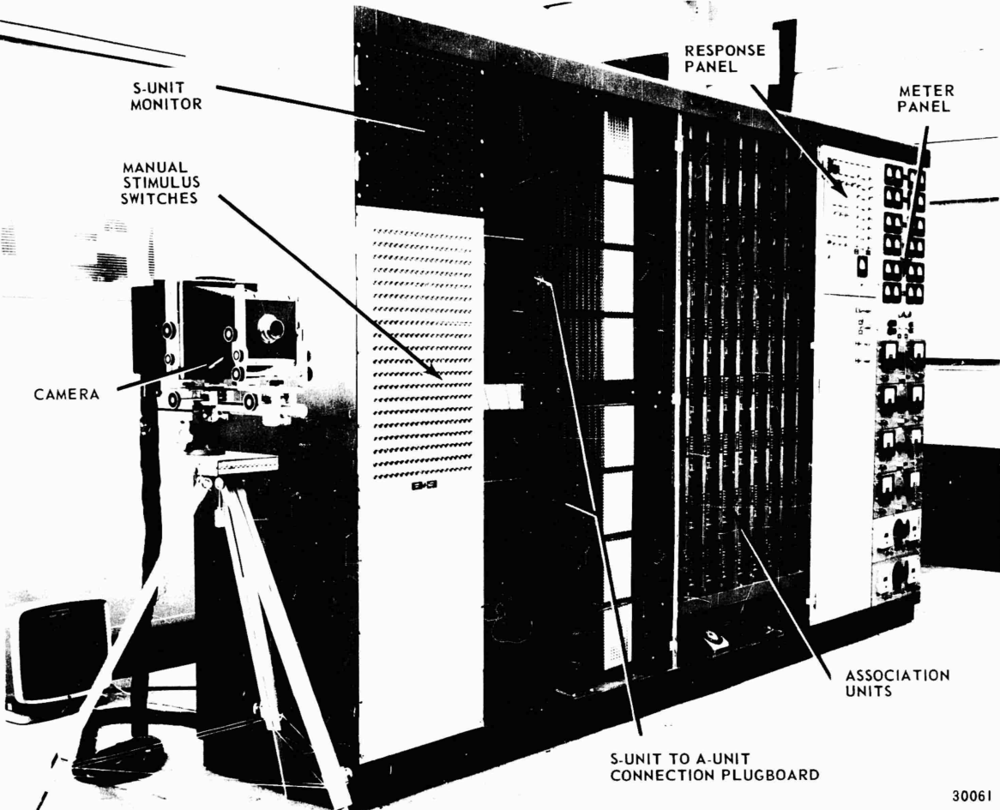
\includegraphics[height=0.40\textheight]{ch13_mark1_perceptron_1960.png}\\[1mm]
\imgcap{The Mark I Perceptron, from its operator's manual}
\imgcredit{https://commons.wikimedia.org/wiki/File:Mark_I_Perceptron,_Figure_2_of_operator\%27s_manual.png}{Figure: J.C. Hay, A.E. Murray (1960); public domain; Wikimedia Commons}
\end{column}
\end{columns}
\end{frame}

\begin{frame}{Two Cultures of Statistical Modelling}
\itemsize{\footnotesize}
\begin{columns}[T]
\begin{column}{0.60\textwidth}
\begin{itemize}
    \item \refBreimanTC, a statistician at Berkeley, describes two cultures
    \begin{itemize}
        \item \textbf{data modelling}: assume a stochastic model (the linear regression $y = x^\top\beta + \varepsilon$, GARCH), estimate it, test its parameters
        \item \textbf{algorithmic modelling}: treat the mechanism as unknown; find a rule $\hat f$ that predicts $y$ well on new data
    \end{itemize}
    \item This course used the first culture in \sfmchlink{https://danpele.github.io/SFM/EN/Courses/chapter2_classical_distributions_stylised_facts.pdf}{Chapters 2}--\sfmchlink{https://danpele.github.io/SFM/EN/Courses/chapter11_fractal_markets_long_memory.pdf}{11}
    \begin{itemize}
        \item this chapter adds the second, and asks when it pays off in finance
    \end{itemize}
\end{itemize}
\end{column}
\begin{column}{0.36\textwidth}
\centering
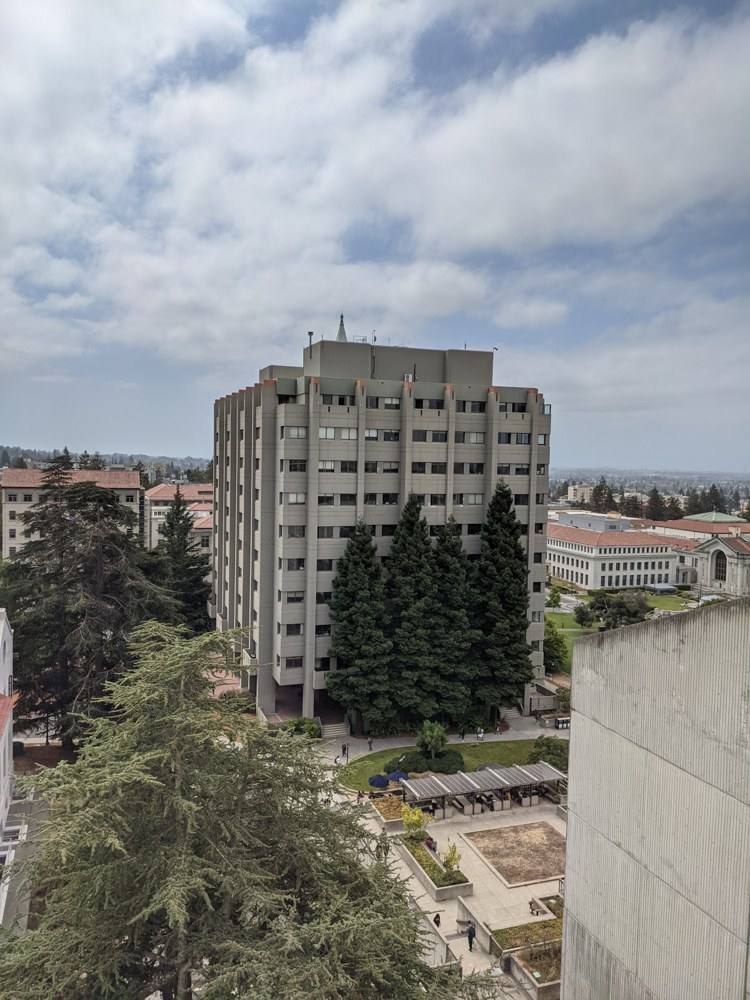
\includegraphics[height=0.46\textheight]{ch13_evans_hall_2021.jpg}\\[1mm]
\imgcap{Evans Hall, University of California, Berkeley, home of the Department of Statistics}
\imgcredit{https://commons.wikimedia.org/wiki/File:Evans_Hall_(UC_Berkeley).jpg}{Photo: Gabriel Classon (2021); CC BY 2.0; Wikimedia Commons}
\end{column}
\end{columns}
\end{frame}

\begin{frame}{Prediction against Inference}
\itemsize{\small}
\begin{itemize}
    \item \textbf{Inference}: is $\beta_j \ne 0$? how large is the effect? (standard errors, tests, \sfmchlink{https://danpele.github.io/SFM/EN/Courses/chapter6_model_selection_risk_management.pdf}{Chapter 6})
    \begin{itemize}
        \item example: does the leverage effect exist (GJR-GARCH, \sfmchlink{https://danpele.github.io/SFM/EN/Courses/chapter9_arch_garch_models.pdf}{Chapter 9})?
    \end{itemize}
    \item \textbf{Prediction}: how close is $\hat y$ to $y$ on data the model has never seen?
    \begin{itemize}
        \item example: next week's volatility; tomorrow's VaR 1\%
        \item the coefficients may be uninterpretable; what matters is the error on new data
    \end{itemize}
    \item The two goals can conflict
    \begin{itemize}
        \item a biased estimator (ridge, lasso) can predict better than the unbiased OLS
        \item a model that predicts well does not prove a causal mechanism
    \end{itemize}
\end{itemize}
\end{frame}

\begin{frame}{Supervised Learning: Notation and Loss (1/2)}
\itemsize{\small}
\begin{itemize}
    \item Data $(x_t, y_t)$, $t = 1, \dots, n$
    \begin{itemize}
        \item $t$: the index of the observation (a day, a week); $n$: the number of observations
        \item $x_t \in \mathbb{R}^p$: the \textbf{features}, $p$ numbers known at time $t$ (past volatilities, past returns)
        \item $y_t$: the \textbf{target}, the quantity we want to forecast (next week's volatility)
    \end{itemize}
    \item Two types of problems
    \begin{itemize}
        \item \textbf{regression}: $y$ continuous (volatility, return)
        \item \textbf{classification}: $y$ a class (up/down, default; \sfmchlink{https://danpele.github.io/SFM/EN/Courses/chapter12_scoring_models.pdf}{Chapter 12})
    \end{itemize}
\end{itemize}
\end{frame}

\begin{frame}{Supervised Learning: Notation and Loss (2/2)}
\itemsize{\small}
\begin{itemize}
    \item Learning = choose $\hat f$ in a family $\mathcal{F}$ that minimises the average \textbf{loss} $\frac1n\sum_t L(y_t, f(x_t))$
    \begin{itemize}
        \item $f(x_t)$: the forecast of a rule $f$ for observation $t$; $L(y, \hat y)$: the cost of forecasting $\hat y$ when $y$ is observed
        \item $\mathcal{F}$: the candidate rules (all linear regressions, all trees of depth 3); $\hat f$: the rule chosen from the data
    \end{itemize}
    \item Losses used in this course
    \begin{itemize}
        \item squared error $(y - \hat y)^2$ (MSE: mean squared error); QLIKE for variances (\sfmchlink{https://danpele.github.io/SFM/EN/Courses/chapter8_volatility_estimators.pdf}{Chapter 8})
        \item quantile (pinball) loss for VaR (\sfmchlink{https://danpele.github.io/SFM/EN/Courses/chapter10_var_es_backtesting.pdf}{Chapter 10}); log loss for probabilities (\sfmchlink{https://danpele.github.io/SFM/EN/Courses/chapter12_scoring_models.pdf}{Chapter 12})
    \end{itemize}
    \item A \textbf{hyperparameter} is chosen before the fit
    \begin{itemize}
        \item examples: tree depth, penalty $\lambda$, number of neurons
        \item the parameters (coefficients, weights) are learned by the fit
    \end{itemize}
\end{itemize}
\end{frame}

\begin{frame}{Where ML Helps in Finance, and Where It Struggles}
\itemsize{\small}
\begin{itemize}
    \item \textbf{Helps}: targets with structure and enough data
    \begin{itemize}
        \item volatility is persistent (\sfmchlink{https://danpele.github.io/SFM/EN/Courses/chapter8_volatility_estimators.pdf}{Chapters 8}--\sfmchlink{https://danpele.github.io/SFM/EN/Courses/chapter9_arch_garch_models.pdf}{9}): a lot to predict, nonlinear effects possible
        \item cross-sections with thousands of stocks and many characteristics (the case study)
    \end{itemize}
    \item \textbf{Struggles}: a low \textbf{signal-to-noise ratio}
    \begin{itemize}
        \item daily returns are close to unpredictable (\sfmchlink{https://danpele.github.io/SFM/EN/Courses/chapter7_efficient_markets_random_walk_vr.pdf}{Chapter 7}): a flexible model fits the noise
        \item markets change (regimes, crises): the past is an imperfect training set
        \item one price history: we cannot repeat the experiment, and the observations are dependent
    \end{itemize}
\end{itemize}
\end{frame}

\begin{frame}{Recap: What Machine Learning Adds}
\itemsize{\small}
\begin{itemize}
    \item ML judges a model by its error on new data, not by the significance of its coefficients
    \item Features $x_t$, target $y_t$, loss $L$, hyperparameters chosen before the fit
    \item Finance: easy to predict volatility, hard to predict returns
\end{itemize}
\end{frame}


%=============================================================================
\section{Overfitting, Bias and Variance}
%=============================================================================

\begin{frame}{Training Error and Test Error}
\itemsize{\small}
\begin{itemize}
    \item \textbf{Training error}: the average loss on the data used for the fit; \textbf{test error}: on new data from the same process
    \begin{itemize}
        \item the training error always falls as the model becomes more flexible
    \end{itemize}
    \item \textbf{Overfitting}: the model learns the noise of the training sample
    \begin{itemize}
        \item symptom: a small training error and a large test error
        \item a tree with one leaf per observation has zero training error and predicts badly
    \end{itemize}
    \item \textbf{Underfitting}: the model is too rigid to capture the signal
    \begin{itemize}
        \item example: a constant forecast of volatility in a world with volatility clustering
    \end{itemize}
\end{itemize}
\end{frame}

\begin{frame}{The Bias--Variance Decomposition (1/2)}
\itemsize{\small}
\begin{itemize}
    \item Model: $y = f(x) + \varepsilon$, $E[\varepsilon] = 0$, $\mathrm{Var}(\varepsilon) = \sigma^2$
    \begin{itemize}
        \item $f$: the true, unknown relation between $x$ and $y$; $\varepsilon$: the noise, unpredictable from $x$, with variance $\sigma^2$
        \item $\hat f$: the estimate of $f$ from a random training sample; another sample would give another $\hat f$
    \end{itemize}
    \item Expected test error at a new point $x_0$, with $y_0 = f(x_0) + \varepsilon_0$: \[ E\big[(y_0 - \hat f(x_0))^2\big] = \underbrace{\big(E[\hat f(x_0)] - f(x_0)\big)^2}_{\text{bias}^2} + \underbrace{\mathrm{Var}\big(\hat f(x_0)\big)}_{\text{variance}} + \underbrace{\sigma^2}_{\text{noise}} \]
    \begin{itemize}
        \item $E[\cdot]$: the average over all possible training samples and over the noise $\varepsilon_0$
        \item bias: how far the average estimate is from the truth; variance: how much $\hat f(x_0)$ moves from one sample to another
    \end{itemize}
\end{itemize}
\end{frame}

\begin{frame}{The Bias--Variance Decomposition (2/2)}
\itemsize{\small}
\begin{itemize}
    \item Derivation: write $y_0 - \hat f = (f - E\hat f) + (E\hat f - \hat f) + \varepsilon_0$, all at $x_0$
    \begin{itemize}
        \item square and take the expectation: the three squares give bias$^2$, variance and $\sigma^2$
        \item the cross terms have mean 0: $E[E\hat f - \hat f] = 0$, and $\varepsilon_0$ is independent of the training sample
    \end{itemize}
    \item Reading the decomposition
    \begin{itemize}
        \item a rigid model: large bias, small variance
        \item a flexible model: small bias, large variance
        \item $\sigma^2$ is the floor: no model goes below it; in daily returns $\sigma^2$ is almost everything
    \end{itemize}
\end{itemize}
\end{frame}

\begin{frame}{Bias and Variance of Regression Trees}
\itemsize{\footnotesize}
\begin{center}
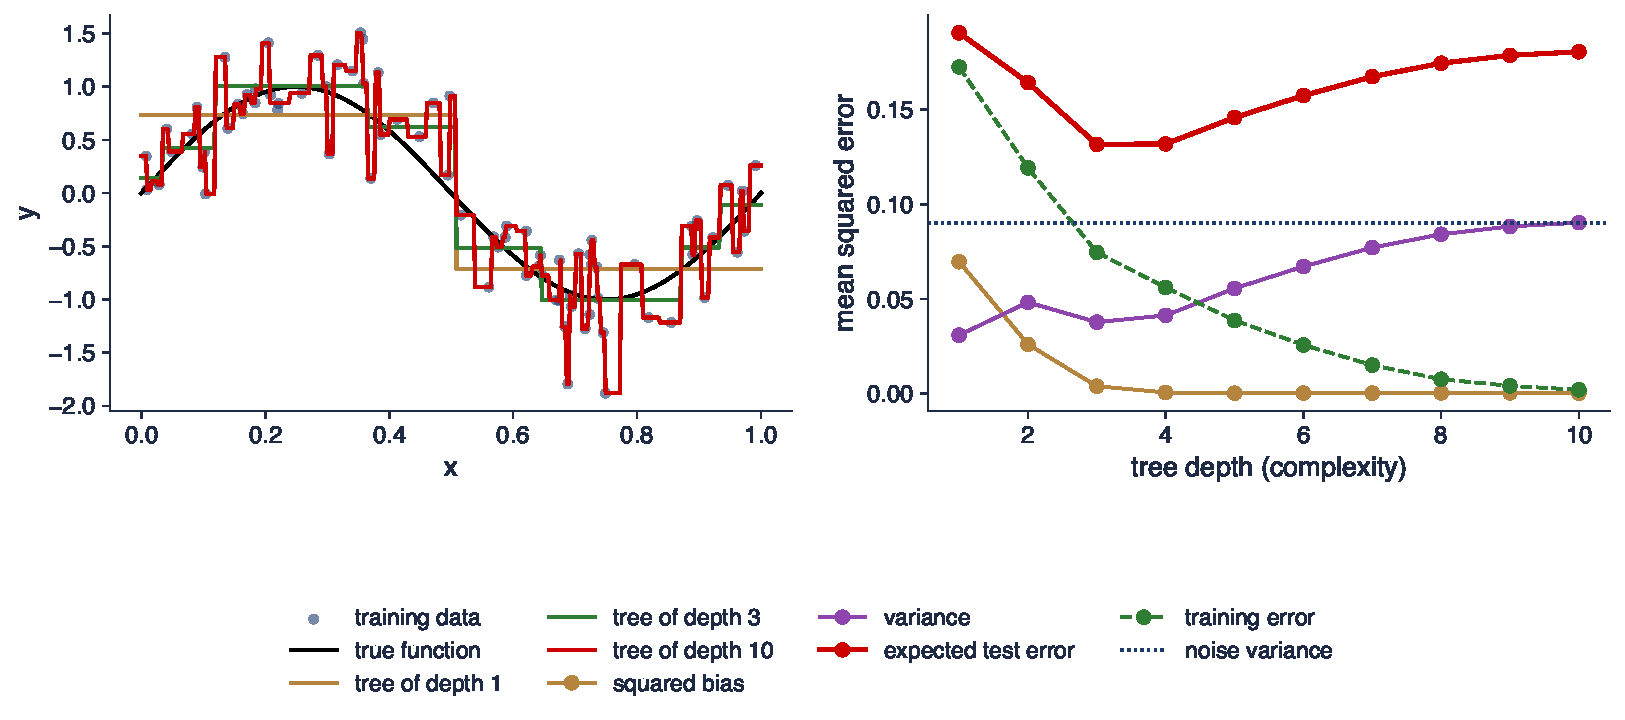
\includegraphics[width=0.97\textwidth,height=0.50\textheight,keepaspectratio]{sfm_ch13_bias_variance.pdf}
\end{center}
\vspace{-0.25cm}
\begin{itemize}
    \item Simulation: $y = \sin(2\pi x) + \varepsilon$, $\sigma^2 = 0.09$, $n = 80$, 300 training samples; left: one sample with trees of depth 1, 3 and 10
    \item Depth 1: bias$^2$ $0.070$, variance $0.031$; depth 10: bias$^2$ $0.000$, variance $0.090$; the test error is smallest at depth 3 ($0.132$)
\end{itemize}
\sfmquantlet{Ch_13}{SFM_ch13_validation}
\end{frame}

\begin{frame}{Interpretation: the U-Shaped Test Error}
\itemsize{\small}
\begin{itemize}
    \item The training error falls from $0.172$ to $0.002$; the test error falls, then rises
    \begin{itemize}
        \item depth 10 has almost zero training error and a test error of $0.180$, worse than depth 3
    \end{itemize}
    \item Consequences for practice
    \begin{itemize}
        \item never select a model by its training error
        \item complexity is a hyperparameter: choose it on data that were not used for the fit
        \item in finance the noise is large, so the best model is usually simpler than in this simulation
    \end{itemize}
\end{itemize}
\end{frame}

\begin{frame}{Recap: Overfitting, Bias and Variance}
\itemsize{\small}
\begin{itemize}
    \item Test error = bias$^2$ + variance + noise
    \item More flexibility: less bias, more variance; the training error is always too optimistic
    \item The amount of flexibility must be chosen on new data
\end{itemize}
\end{frame}


%=============================================================================
\section{Validation for Time Series}
%=============================================================================

\begin{frame}{Training, Validation and Test Samples}
\itemsize{\small}
\begin{itemize}
    \item Three roles for the data
    \begin{itemize}
        \item \textbf{training}: estimate the parameters of each candidate model
        \item \textbf{validation}: choose the hyperparameters and the model
        \item \textbf{test}: measure the error of the final choice, once
    \end{itemize}
    \item Every look at the test sample turns it into a validation sample
    \begin{itemize}
        \item trying ten models on the test data and reporting the best is model selection, not testing
    \end{itemize}
    \item \textbf{K-fold cross-validation}: split the data into $K$ folds; each fold is the validation set once, the others train the model
    \begin{itemize}
        \item valid for i.i.d.\ data; for a time series only under strong conditions (no dependence left in the errors) \refBHK
    \end{itemize}
\end{itemize}
\end{frame}

\begin{frame}{Look-Ahead Bias and Leakage}
\itemsize{\small}
\begin{itemize}
    \item \textbf{Look-ahead bias}: the forecast for day $t$ uses information that was not available at the close of day $t - 1$
    \begin{itemize}
        \item features computed with future prices (a centred moving average, a full-sample mean)
        \item scaling or standardising with statistics of the whole sample; revised data; today's index members (survivorship)
    \end{itemize}
    \item \textbf{Leakage}: information about the test target reaches the training sample
    \begin{itemize}
        \item overlapping targets: the 21-day return from day $t$ and from day $t + 1$ share 20 days
        \item a random fold puts day $t + 1$ in training and day $t$ in test: the model has seen the answer
    \end{itemize}
    \item Both make a model look better than it can be in real time
\end{itemize}
\end{frame}

\begin{frame}{Three Validation Schemes}
\itemsize{\footnotesize}
\begin{center}
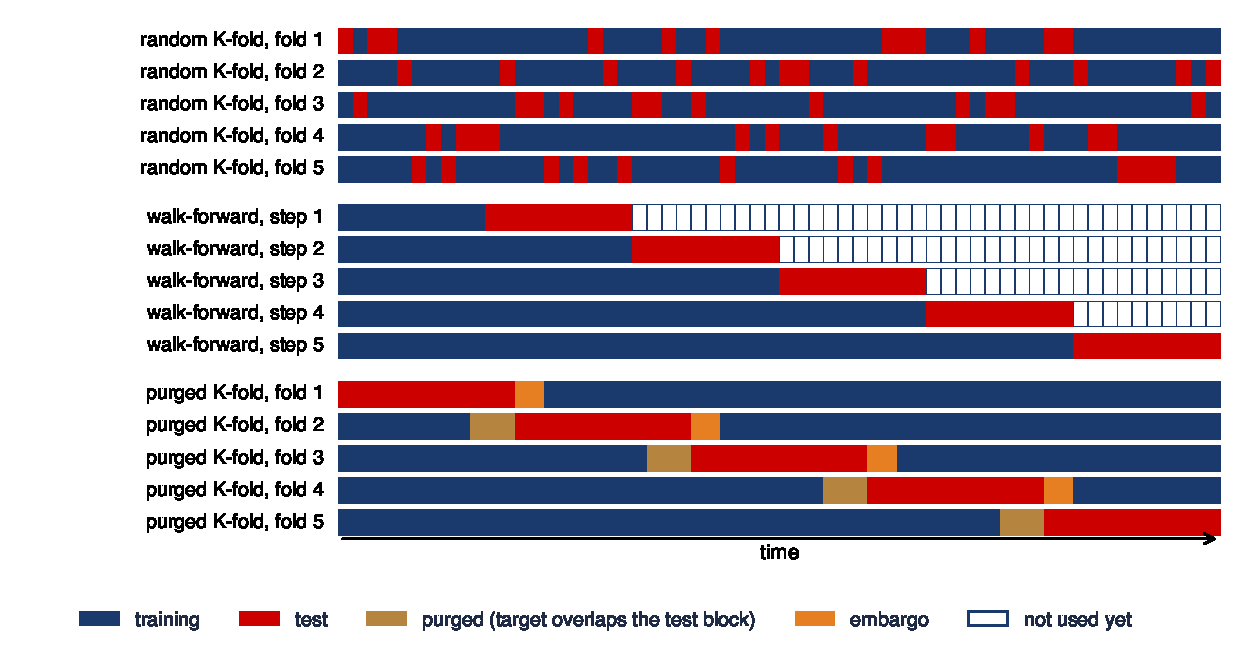
\includegraphics[width=0.97\textwidth,height=0.52\textheight,keepaspectratio]{sfm_ch13_cv_schemes.pdf}
\end{center}
\vspace{-0.25cm}
\begin{itemize}
    \item \textbf{Walk-forward}: train on the past, test on the next block, move forward; the expanding window keeps all the past
    \item \textbf{Purged K-fold with embargo} \refLdP: drop the training rows whose targets overlap the test block (purging) and a few rows after it (embargo)
\end{itemize}
\sfmquantlet{Ch_13}{SFM_ch13_validation}
\end{frame}

\begin{frame}{Walk-Forward Validation, Step by Step}
\itemsize{\small}
\begin{itemize}
    \item The design used in this chapter for the S\&P 500 (data from 8 April 2008)
    \begin{itemize}
        \item one fold per calendar year from 2013: 14 folds; the model is re-estimated each January
        \item training window: all earlier days (expanding); test: every day of the year
    \end{itemize}
    \item Purging: the target is the mean variance of the next 5 days
    \begin{itemize}
        \item for 2013 the last 5 training rows (from 24 December 2012) are dropped: their targets reach into 2013
        \item the 2013 fold trains on 1\,188 days and tests on 252; the 2026 fold trains on 4\,458 days
    \end{itemize}
    \item Inside each training window, hyperparameters are tuned by a walk-forward split of the training data only
    \begin{itemize}
        \item no embargo is needed: the test block always comes after the training block
    \end{itemize}
\end{itemize}
\end{frame}

\begin{frame}{Leakage in Practice: Random Folds on Overlapping Targets}
\itemsize{\footnotesize}
\begin{center}
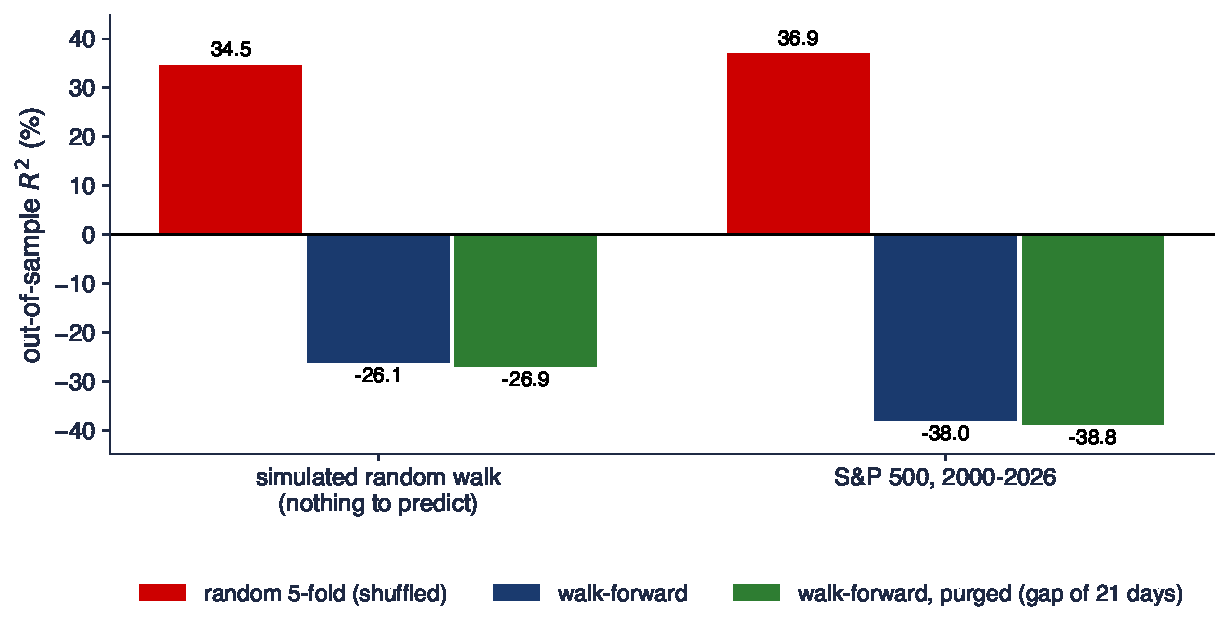
\includegraphics[width=0.97\textwidth,height=0.48\textheight,keepaspectratio]{sfm_ch13_leakage.pdf}
\end{center}
\vspace{-0.25cm}
\begin{itemize}
    \item Random forest for the next 21-day return from past returns and volatilities; out-of-sample $R^2$ against the training mean
    \item Simulated random walk: random 5-fold $34.5\%$, walk-forward $-26.1\%$; S\&P 500 (6\,631 days): $36.9\%$ and $-38.0\%$
\end{itemize}
\sfmquantlet{Ch_13}{SFM_ch13_validation}
\end{frame}

\begin{frame}{Interpretation: a Forecast of Pure Noise with $R^2 > 30\%$}
\itemsize{\small}
\begin{itemize}
    \item The random walk has nothing to predict, yet random folds report $R^2 = 34.5\%$
    \begin{itemize}
        \item the forest memorises neighbouring days, whose targets share 20 of 21 returns with the test day
    \end{itemize}
    \item Walk-forward gives a negative $R^2$: the forest fits noise and loses against the training mean
    \begin{itemize}
        \item purging (a gap of 21 days) changes little here, because in walk-forward only the boundary rows overlap
    \end{itemize}
    \item Rule: with overlapping targets or dependent data, never shuffle the time order
\end{itemize}
\end{frame}

\begin{frame}{Recap: Validation for Time Series}
\itemsize{\small}
\begin{itemize}
    \item Training, validation and test have different jobs; the test sample is used once
    \item Walk-forward with purging respects the arrow of time; random K-fold leaks with overlapping targets
    \item Look-ahead bias and leakage produce impressive but useless results
\end{itemize}
\end{frame}


%=============================================================================
\section{Penalised Regression: Ridge and Lasso}
%=============================================================================

\begin{frame}{Many Features, Unstable OLS}
\itemsize{\small}
\begin{itemize}
    \item OLS (ordinary least squares): $\hat\beta = \arg\min_\beta \sum_t (y_t - x_t^\top\beta)^2 = (X^\top X)^{-1}X^\top y$
    \begin{itemize}
        \item $X$: the $n \times p$ matrix whose row $t$ is $x_t^\top$; $y$: the vector of targets; $\arg\min_\beta$: the $\beta$ that minimises the sum
        \item unbiased, but its variance $\sigma^2(X^\top X)^{-1}$ ($\sigma^2$: the error variance) explodes when features are many or strongly correlated
    \end{itemize}
    \item Volatility features are highly correlated: today's, this week's and this month's realised variance
    \begin{itemize}
        \item OLS may give large coefficients of opposite signs that cancel in sample and fail out of sample
    \end{itemize}
    \item \textbf{Penalised regression}: minimise the squared error plus a penalty on the size of $\beta$
    \begin{itemize}
        \item accept a little bias for a large reduction in variance (the trade-off of Section 2)
    \end{itemize}
\end{itemize}
\end{frame}

\begin{frame}{Ridge Regression (1/2)}
\itemsize{\small}
\begin{itemize}
    \item \refHK: minimise the squared error plus a penalty on the squared coefficients \[ \hat\beta^{\,ridge} = \arg\min_\beta \sum_t (y_t - x_t^\top\beta)^2 + \lambda\sum_j \beta_j^2 = (X^\top X + \lambda I)^{-1}X^\top y \]
    \item Notation
    \begin{itemize}
        \item $\beta_j$: the coefficient of feature $j$; $\sum_j \beta_j^2$: the penalty term, large when the coefficients are large
        \item $\lambda \ge 0$: the strength of the penalty; $\lambda = 0$ gives OLS, $\lambda \to \infty$ gives $\hat\beta \to 0$
        \item $I$: the $p \times p$ identity matrix
    \end{itemize}
    \item Consequence
    \begin{itemize}
        \item $X^\top X + \lambda I$ is always invertible for $\lambda > 0$: ridge works even with more features than observations
    \end{itemize}
\end{itemize}
\end{frame}

\begin{frame}{Ridge Regression (2/2)}
\itemsize{\small}
\begin{itemize}
    \item \textbf{One feature}, centred (mean 0): $S_{xx} = \sum_t x_t^2$, $S_{xy} = \sum_t x_ty_t$ \[ \hat\beta^{\,ridge} = \dfrac{S_{xy}}{S_{xx} + \lambda} = \dfrac{S_{xx}}{S_{xx} + \lambda}\,\hat\beta^{\,OLS}, \qquad \hat\beta^{\,OLS} = \dfrac{S_{xy}}{S_{xx}} \]
    \begin{itemize}
        \item the factor $S_{xx}/(S_{xx} + \lambda)$ lies in $(0, 1]$: the share of the OLS coefficient that ridge keeps
    \end{itemize}
    \item Example: $S_{xx} = 100$, $S_{xy} = 30$
    \begin{itemize}
        \item OLS: $30/100 = 0.30$
        \item ridge with $\lambda = 50$: $30/150 = 0.20$ (shrinkage factor $0.67$)
    \end{itemize}
    \item Ridge shrinks all coefficients towards zero, but sets none exactly to zero
\end{itemize}
\end{frame}

\begin{frame}{The Lasso}
\itemsize{\footnotesize}
\begin{columns}[T]
\begin{column}{0.64\textwidth}
\begin{itemize}
    \item \refTib: $\hat\beta^{\,lasso} = \arg\min_\beta \sum_t (y_t - x_t^\top\beta)^2 + \lambda\sum_j |\beta_j|$
    \begin{itemize}
        \item the absolute value has a kink at 0: some coefficients become \textbf{exactly zero} (variable selection)
    \end{itemize}
    \item One feature: \textbf{soft thresholding}
    \begin{itemize}
        \item $\hat\beta^{\,lasso} = \mathrm{sign}(S_{xy})\,\max(|S_{xy}| - \lambda/2,\, 0)/S_{xx}$
        \item $\mathrm{sign}(S_{xy})$: $+1$ or $-1$; if $|S_{xy}| \le \lambda/2$, the coefficient is exactly 0
        \item same data, $\lambda = 20$: $(30 - 10)/100 = 0.20$; zero for $\lambda \ge 60$
    \end{itemize}
    \item In practice
    \begin{itemize}
        \item standardise the features first (the penalty depends on their units), with the training mean and standard deviation only
        \item choose $\lambda$ by walk-forward cross-validation; elastic net combines both penalties
    \end{itemize}
\end{itemize}
\end{column}
\begin{column}{0.32\textwidth}
\centering
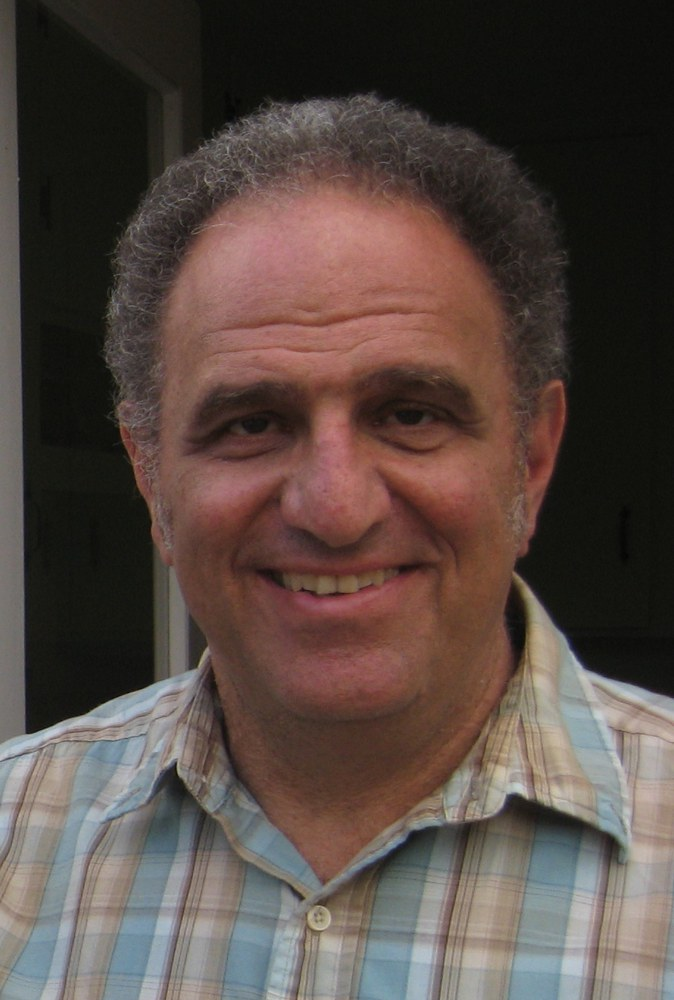
\includegraphics[height=0.42\textheight]{ch13_tibshirani_2012.jpg}\\[1mm]
\imgcap{Robert Tibshirani, Stanford University}
\imgcredit{https://commons.wikimedia.org/wiki/File:Robert_tibshirani.jpg}{Photo: R. Tibshirani (2012); CC BY-SA 3.0; Wikimedia Commons}
\end{column}
\end{columns}
\end{frame}

\begin{frame}{Ridge and Lasso Paths for the Volatility Features}
\itemsize{\footnotesize}
\begin{center}
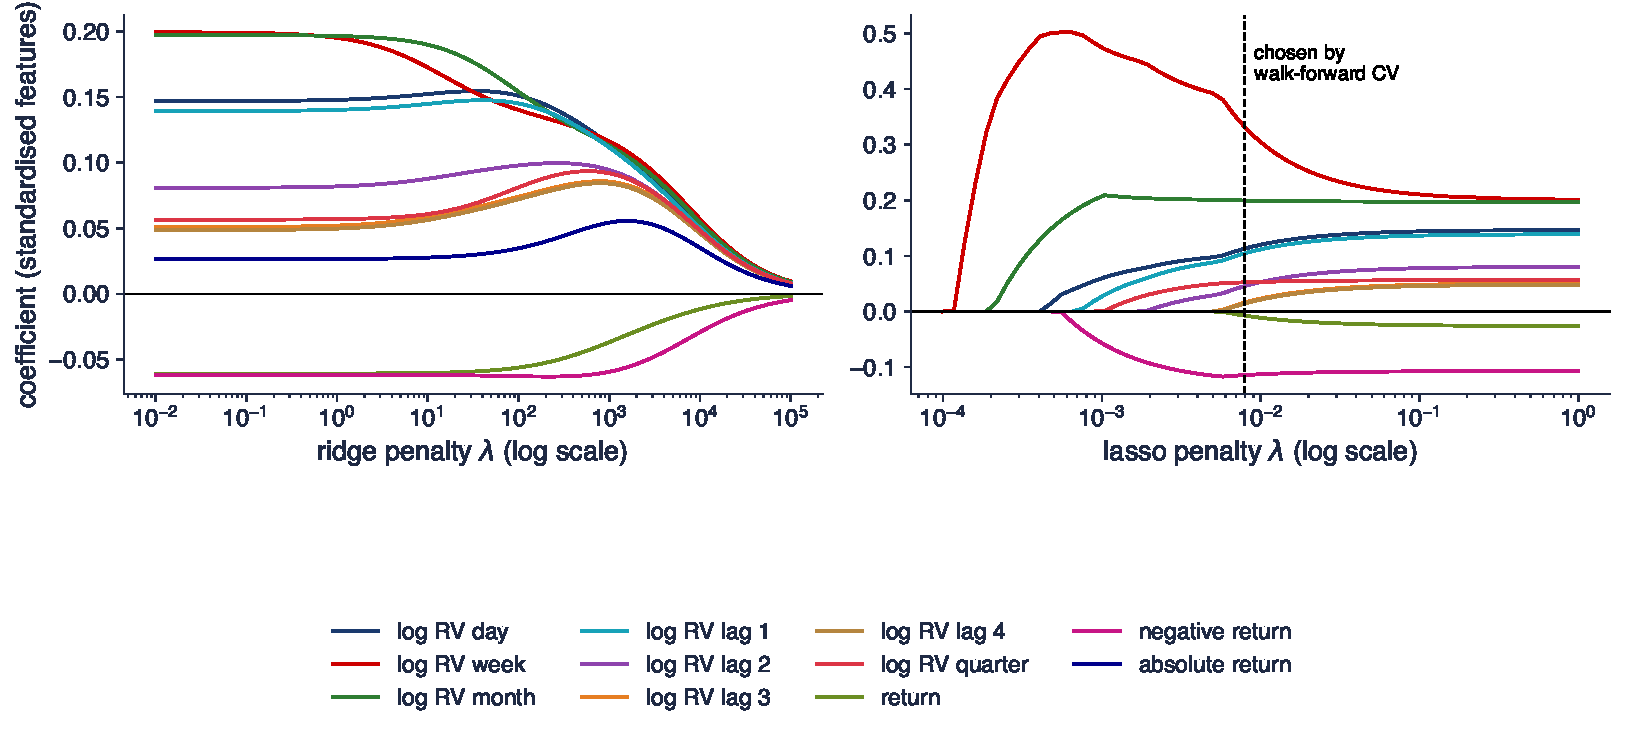
\includegraphics[width=0.97\textwidth,height=0.50\textheight,keepaspectratio]{sfm_ch13_shrinkage.pdf}
\end{center}
\vspace{-0.25cm}
\begin{itemize}
    \item Target: log of the mean variance proxy of the next 5 days, S\&P 500, 2008--2012 (1\,193 days); 11 standardised features (Section 7)
    \item Lasso with $\lambda = 0.0079$ (walk-forward CV): 10 of 11 features kept; the week coefficient rises from $+0.199$ (OLS) to $+0.283$, the absolute return drops out
\end{itemize}
\sfmquantlet{Ch_13}{SFM_ch13_shrinkage_trees}
\end{frame}

\begin{frame}{Interpretation of the Paths}
\itemsize{\small}
\begin{itemize}
    \item Ridge (left): all coefficients shrink smoothly and together; correlated features share the weight
    \begin{itemize}
        \item the negative return keeps a negative sign until the end: falling markets raise future volatility (the leverage effect, \sfmchlink{https://danpele.github.io/SFM/EN/Courses/chapter9_arch_garch_models.pdf}{Chapter 9})
    \end{itemize}
    \item Lasso (right): the features enter one by one as $\lambda$ falls
    \begin{itemize}
        \item the weekly variance enters first: the most informative single feature
        \item at the chosen $\lambda$ the lasso keeps the HAR structure (day, week, month) plus the negative return, $-0.112$
    \end{itemize}
    \item The lasso selects; it does not test: a zero coefficient is not a p-value
\end{itemize}
\end{frame}

\begin{frame}{Recap: Ridge and Lasso}
\itemsize{\small}
\begin{itemize}
    \item Penalties trade a little bias for less variance: $\lambda\sum\beta_j^2$ (ridge), $\lambda\sum|\beta_j|$ (lasso)
    \item Ridge shrinks, lasso shrinks and selects; standardise first, choose $\lambda$ by walk-forward CV
    \item For volatility, the penalised model keeps the HAR structure and the leverage effect
\end{itemize}
\end{frame}


%=============================================================================
\section{Trees, Random Forest and Gradient Boosting}
%=============================================================================

\begin{frame}{Regression Trees}
\itemsize{\small}
\begin{itemize}
    \item A \textbf{regression tree} splits the feature space into rectangles and predicts the mean of $y$ in each \textbf{leaf}
    \begin{itemize}
        \item split rule: a feature $j$ and a threshold $s$: left $x_j \le s$, right $x_j > s$
    \end{itemize}
    \item \textbf{Greedy fit}: at each node choose $(j, s)$ that minimises $\mathrm{SSE} = \sum_{\text{left}}(y - \bar y_L)^2 + \sum_{\text{right}}(y - \bar y_R)^2$
    \begin{itemize}
        \item SSE: sum of squared errors; $\bar y_L$, $\bar y_R$: the means of $y$ in the left and right groups (the two forecasts)
        \item repeat in each half until a stopping rule: maximum depth, minimum number of observations per leaf
    \end{itemize}
    \item Strengths and weaknesses
    \begin{itemize}
        \item nonlinear effects and interactions without specifying them; insensitive to monotone transformations of $x$
        \item high variance: a small change in the data can change the whole tree (Section 2)
    \end{itemize}
\end{itemize}
\end{frame}

\begin{frame}{Worked Example: One Split, Step by Step}
\itemsize{\footnotesize}
\begin{columns}[T]
\begin{column}{0.42\textwidth}
\begin{center}
\footnotesize
\begin{tabular}{rrrr}
\toprule
$s$ & $\bar y_L$ & $\bar y_R$ & SSE \\
\midrule
$0.70$ & $0.70$ & $1.52$ & $1.708$ \\
$0.90$ & $0.80$ & $1.68$ & $1.248$ \\
$1.25$ & $0.80$ & $1.97$ & $0.227$ \\
$1.75$ & $1.00$ & $2.15$ & $0.505$ \\
$2.20$ & $1.22$ & $2.20$ & $1.468$ \\
\bottomrule
\end{tabular}
\end{center}

\end{column}
\begin{column}{0.56\textwidth}
\begin{itemize}
    \item Six weeks: $x$ = this week's volatility (\%), $y$ = next week's
    \begin{itemize}
        \item $x$: 0.6, 0.8, 1.0, 1.5, 2.0, 2.4; $y$: 0.7, 0.9, 0.8, 1.6, 2.1, 2.2
        \item no split: $\bar y = 1.38$, SSE $= 2.268$
    \end{itemize}
    \item Candidates: the midpoints between consecutive $x$ values
    \begin{itemize}
        \item best split $s = 1.25$: leaves $0.80$ and $1.97$, SSE $= 0.227$
        \item one split explains $1 - 0.227/2.268 = 0.90$ of the variation
    \end{itemize}
\end{itemize}
\end{column}
\end{columns}
\end{frame}

\begin{frame}{A Depth-2 Tree for Next Week's Volatility}
\itemsize{\footnotesize}
\begin{center}
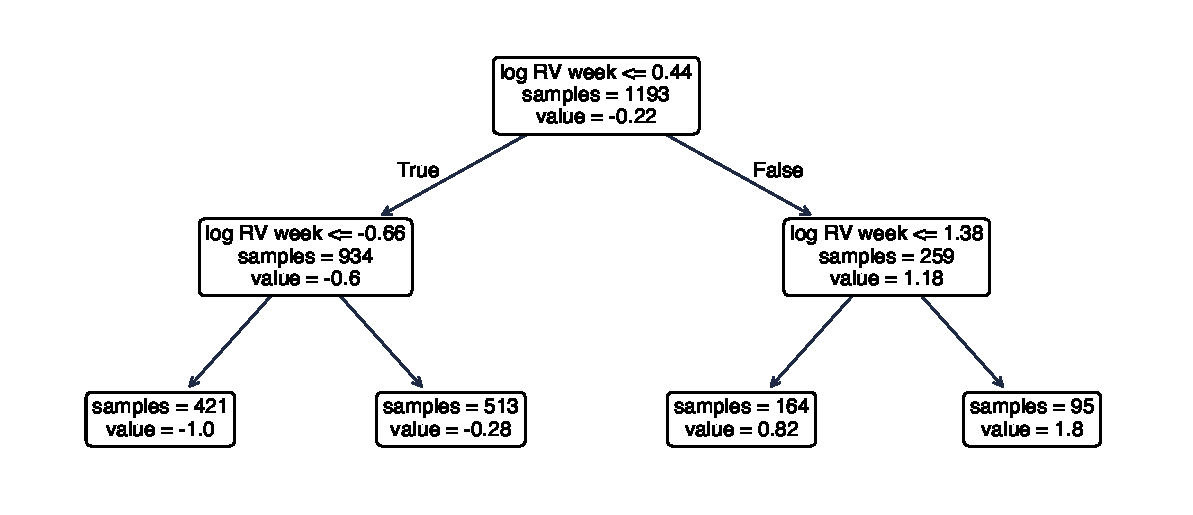
\includegraphics[width=0.97\textwidth,height=0.50\textheight,keepaspectratio]{sfm_ch13_tree.pdf}
\end{center}
\vspace{-0.25cm}
\begin{itemize}
    \item S\&P 500, 2008--2012, target and features in log variance (\%$^2$ per day); \emph{value}: the mean of the target in the node
    \item Interpretation: the first split, log RV week $\le 0.44$, is an annual volatility of about 19.8\%; all splits use the weekly variance, the feature the lasso picked first
\end{itemize}
\sfmquantlet{Ch_13}{SFM_ch13_shrinkage_trees}
\end{frame}

\begin{frame}{Random Forest}
\itemsize{\small}
\begin{itemize}
    \item \refBreiman: average $B$ deep trees, each grown on a bootstrap sample (\sfmchlink{https://danpele.github.io/SFM/EN/Courses/chapter2_classical_distributions_stylised_facts.pdf}{Chapter 2}) of the training data (\textbf{bagging})
    \begin{itemize}
        \item at each split only a random subset of the features is tried: the trees become less correlated
    \end{itemize}
    \item Why averaging works: $B$ trees, each with variance $\sigma^2$ and pairwise correlation $\rho$
    \begin{itemize}
        \item $\mathrm{Var}(\text{average}) = \rho\sigma^2 + (1 - \rho)\sigma^2/B$: the part $\rho\sigma^2$, common to all trees, does not fall with $B$
        \item with $\rho = 0.3$, $\sigma^2 = 1$: $B = 1$: $1.000$; $B = 10$: $0.370$; $B = 300$: $0.302$
        \item more trees never overfit; less correlated trees (fewer features per split) reduce the floor $\rho\sigma^2$
    \end{itemize}
    \item Hyperparameters used here: 300 trees, at least 20 observations per leaf, half of the features tried at each split
\end{itemize}
\end{frame}

\begin{frame}{Gradient Boosting}
\itemsize{\small}
\begin{itemize}
    \item \refFriedman: build the model step by step, each new small tree fitting what the previous ones missed
    \begin{itemize}
        \item start with $F_0 = \bar y$; at step $m$, fit a shallow tree $h_m$ to the residuals $y_t - F_{m-1}(x_t)$
        \item update $F_m = F_{m-1} + \nu\, h_m$, with the \textbf{learning rate} $0 < \nu \le 1$
        \item for squared loss the residuals are minus the gradient of the loss: hence the name
    \end{itemize}
    \item Random forest against boosting
    \begin{itemize}
        \item forest: deep trees in parallel, averaging reduces variance
        \item boosting: shallow trees in sequence, each step reduces bias; too many steps overfit
    \end{itemize}
    \item Any differentiable loss works: quantile loss gives quantile boosting (Section 9)
\end{itemize}
\end{frame}

\begin{frame}{One Tree, a Forest and Boosting on Volatility Data}
\itemsize{\footnotesize}
\begin{center}
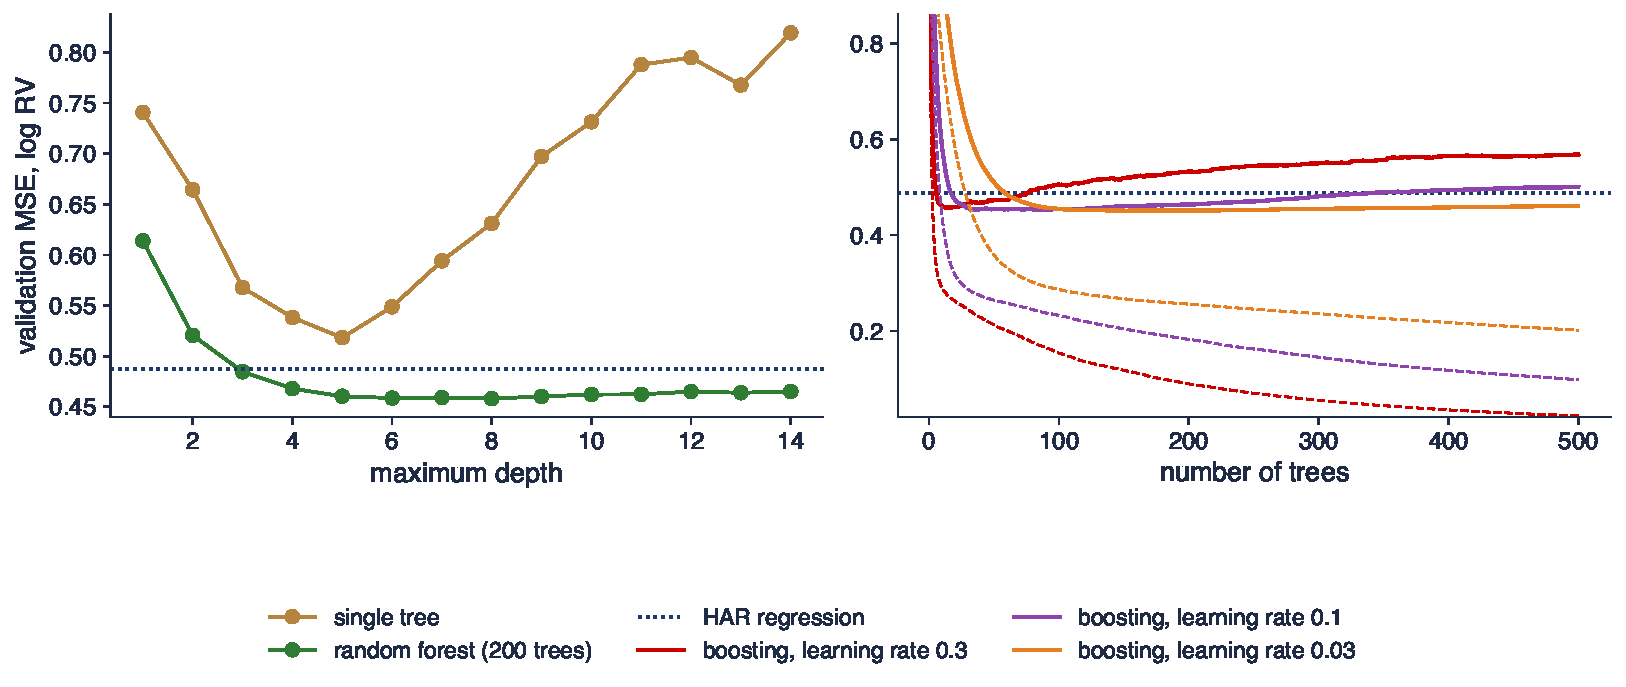
\includegraphics[width=0.97\textwidth,height=0.48\textheight,keepaspectratio]{sfm_ch13_ensembles.pdf}
\end{center}
\vspace{-0.25cm}
\begin{itemize}
    \item S\&P 500, training 2008--2018 (2\,698 days), validation 2019--2022 (1\,008 days); dashed right: training MSE; dotted: HAR regression ($0.487$)
    \item Single tree: best $0.518$ at depth 5, $0.819$ at depth 14; forest: $0.458$ (depth 8) and still $0.465$ at depth 14
\end{itemize}
\sfmquantlet{Ch_13}{SFM_ch13_shrinkage_trees}
\end{frame}

\begin{frame}{Interpretation: Averaging and Early Stopping}
\itemsize{\small}
\begin{itemize}
    \item The single tree overfits quickly; the forest is almost insensitive to depth
    \begin{itemize}
        \item averaging removes most of the variance of deep trees; the forest beats HAR on this validation period
    \end{itemize}
    \item Boosting: the validation error reaches its minimum, then rises while the training error keeps falling
    \begin{itemize}
        \item learning rate 0.3: minimum $0.457$ after 13 trees, $0.568$ after 500
        \item learning rate 0.03: minimum $0.451$ after 154 trees, $0.461$ after 500: smaller steps are safer
    \end{itemize}
    \item The number of trees of boosting is a hyperparameter; the number of trees of a forest is not
\end{itemize}
\end{frame}

\begin{frame}{Recap: Trees and Ensembles}
\itemsize{\small}
\begin{itemize}
    \item A tree splits greedily to minimise the SSE; alone it has high variance
    \item Random forest averages decorrelated deep trees; boosting adds shallow trees fitted to residuals
    \item Forest: robust to its hyperparameters; boosting: needs a small learning rate and a validated number of trees
\end{itemize}
\end{frame}


%=============================================================================
\section{Neural Networks}
%=============================================================================

\begin{frame}{From the Perceptron to the Multilayer Perceptron (1/2)}
\itemsize{\small}
\begin{itemize}
    \item A \textbf{neuron}: $h = g(b + w^\top x)$, a weighted sum of the inputs passed through an \textbf{activation function} $g$
    \begin{itemize}
        \item $x$: the inputs; $w$: their weights; $b$: a constant (the bias term of the neuron); $h$: the output of the neuron
        \item $g$: a fixed nonlinear function; without it, a network of neurons would be just a linear regression
    \end{itemize}
    \item Activation functions
    \begin{itemize}
        \item the perceptron uses a step function (0 or 1)
        \item modern networks use smooth or piecewise linear $g$: logistic $1/(1 + e^{-z})$, tanh, ReLU $\max(0, z)$
    \end{itemize}
\end{itemize}
\end{frame}

\begin{frame}{From the Perceptron to the Multilayer Perceptron (2/2)}
\itemsize{\small}
\begin{itemize}
    \item \textbf{MLP} (multilayer perceptron) with one hidden layer of $K$ neurons \[ \hat y = c + \sum_{k=1}^{K} v_k\, g(b_k + w_k^\top x) \]
    \begin{itemize}
        \item $w_k$, $b_k$: the weights and the constant of hidden neuron $k$; $v_k$: the weight of neuron $k$ in the output; $c$: the output constant
        \item reading: a linear model in $K$ nonlinear features $g(b_k + w_k^\top x)$, which are themselves learned
    \end{itemize}
    \item Number of parameters with 11 inputs and 16 neurons
    \begin{itemize}
        \item hidden layer: $11 \times 16$ weights $+ 16$ constants $= 192$; output: $16 + 1 = 17$; total 209
    \end{itemize}
    \item \textbf{Universal approximation} \refHSW: with enough neurons, one hidden layer approximates any continuous function on a compact set
\end{itemize}
\end{frame}

\begin{frame}{A Small Network and Its Activation Functions}
\itemsize{\footnotesize}
\begin{center}
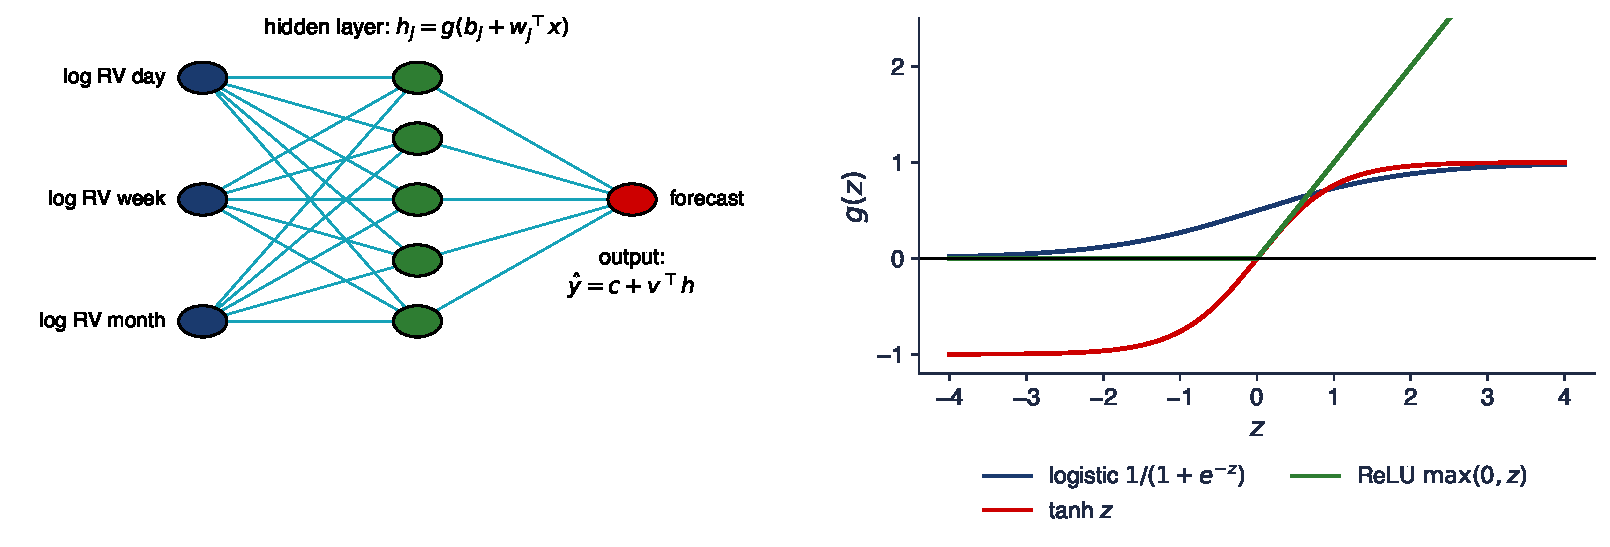
\includegraphics[width=0.97\textwidth,height=0.50\textheight,keepaspectratio]{sfm_ch13_mlp.pdf}
\end{center}
\vspace{-0.25cm}
\begin{itemize}
    \item Left: three HAR inputs, five hidden neurons, one forecast; each line is a weight
    \item Right: logistic and tanh saturate for large $|z|$; ReLU $= \max(0, z)$ is linear for $z > 0$ and trains faster
\end{itemize}
\sfmquantlet{Ch_13}{SFM_ch13_neural_networks}
\end{frame}

\begin{frame}{Training a Network}
\itemsize{\small}
\begin{itemize}
    \item Minimise the loss by \textbf{gradient descent}: $\theta \leftarrow \theta - \eta\,\nabla_\theta L$
    \begin{itemize}
        \item $\theta$: all weights and constants; $\nabla_\theta L$: the gradient, the vector of partial derivatives of the loss; $\eta > 0$: the learning rate (the step size)
        \item each step moves $\theta$ in the direction in which the loss falls fastest
        \item \textbf{back-propagation} computes $\nabla_\theta L$ layer by layer with the chain rule \refRHW
        \item one \textbf{epoch} = one pass over the training data; Adam is a gradient method with adaptive step sizes
    \end{itemize}
    \item The loss is not convex: different starting weights give different networks
    \begin{itemize}
        \item we fix the random seeds and average five networks (an \textbf{ensemble})
    \end{itemize}
    \item Against overfitting
    \begin{itemize}
        \item standardise inputs and target with training statistics; an $L_2$ penalty on the weights (as ridge); a fixed number of epochs
        \item small data, small network: one hidden layer of 16 neurons is enough here
    \end{itemize}
\end{itemize}
\end{frame}

\begin{frame}{From Deep Blue to Deep Learning}
\itemsize{\footnotesize}
\begin{columns}[T]
\begin{column}{0.48\textwidth}
\centering
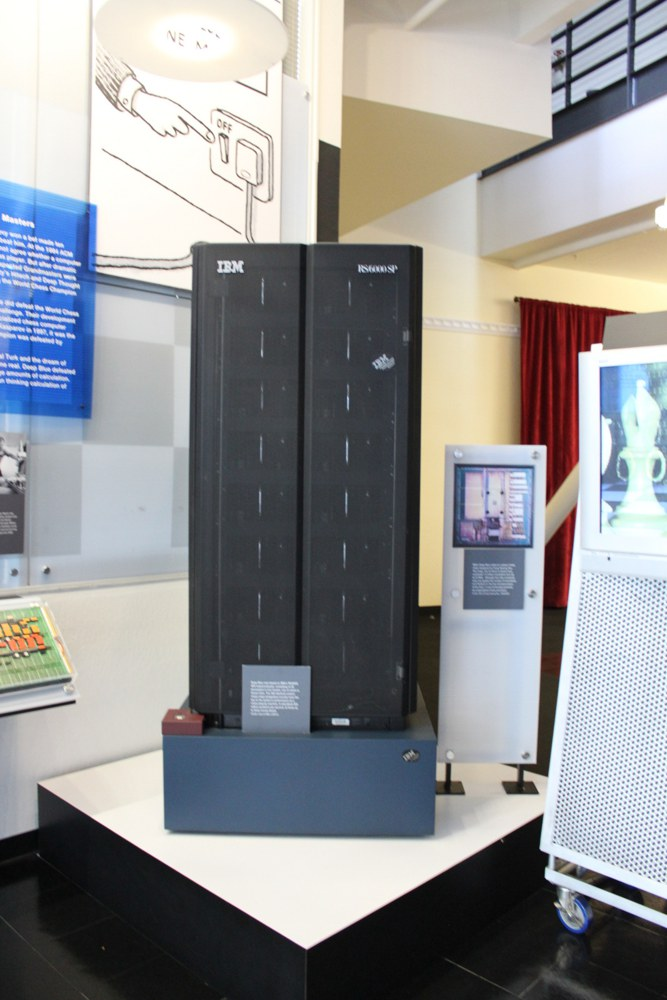
\includegraphics[height=0.36\textheight]{ch13_deep_blue_2011.jpg}\\[1mm]
\imgcap{IBM Deep Blue, Computer History Museum}
\imgcredit{https://commons.wikimedia.org/wiki/File:IBM_Deep_Blue_at_Computer_History_Museum_(9361685537).jpg}{Photo: Anton Chiang (2011); CC BY 2.0; Wikimedia Commons}
\end{column}
\begin{column}{0.48\textwidth}
\centering
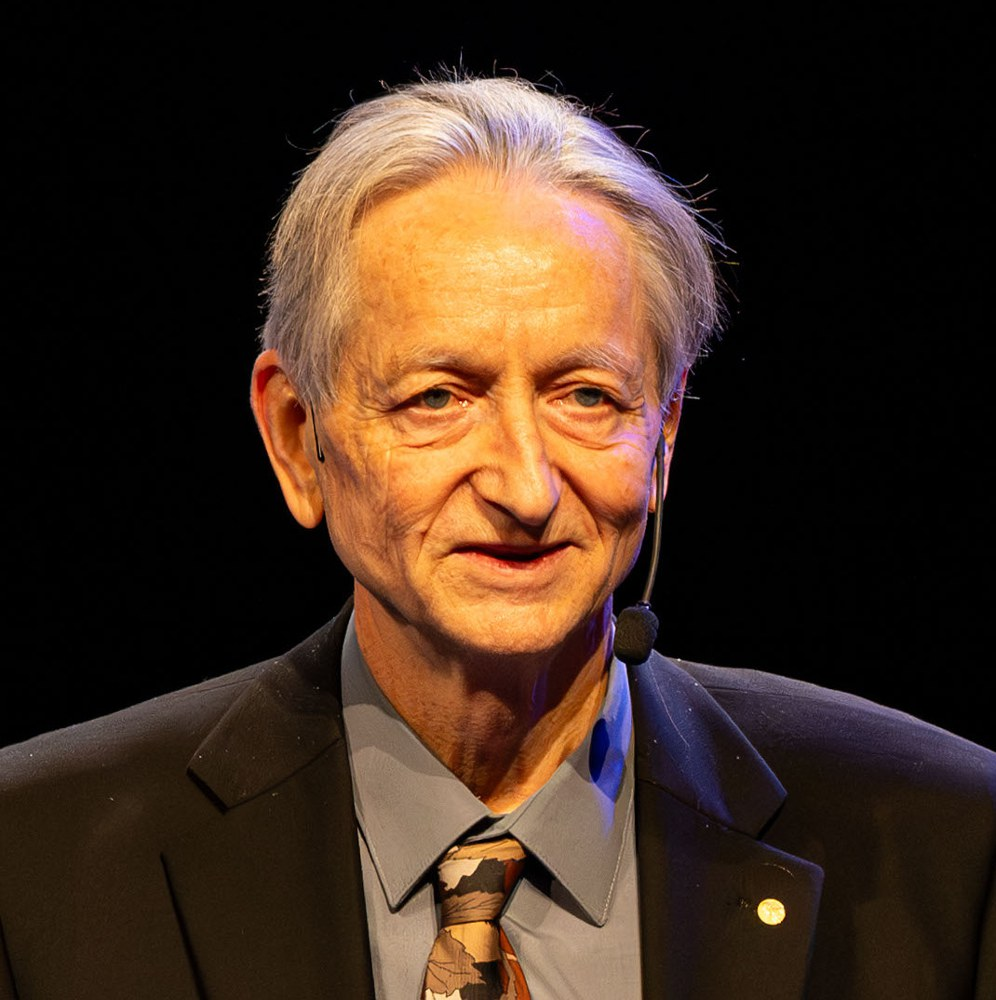
\includegraphics[height=0.36\textheight]{ch13_hinton_2024.jpg}\\[1mm]
\imgcap{Geoffrey Hinton, Nobel Prize in Physics 2024}
\imgcredit{https://commons.wikimedia.org/wiki/File:Geoffrey_E._Hinton,_2024_Nobel_Prize_Laureate_in_Physics_(cropped1).jpg}{Photo: Arthur Petron (2024); CC BY-SA 4.0; Wikimedia Commons}
\end{column}
\end{columns}\begin{itemize}
    \item 1997: Deep Blue beat the world chess champion mainly by search and hand-crafted evaluation rules, not by learning from data
    \item Deep learning (many layers, huge data) now dominates images and text; on financial prices the data are few and noisy, so small networks are the norm
\end{itemize}
\end{frame}

\begin{frame}{Neural-Network ARCH: the Textbook Model (1/2)}
\itemsize{\small}
\begin{itemize}
    \item \refFHH, Ch.~19: $r_t = f(x_{t-1}) + s(x_{t-1})\,\varepsilon_t$, with $f$ and $s^2$ estimated by neural networks
    \begin{itemize}
        \item $r_t$: the return of day $t$; $x_{t-1}$: the inputs known at the close of day $t - 1$
        \item $f(x_{t-1})$: the conditional mean; $s^2(x_{t-1})$: the conditional variance; $\varepsilon_t$: a shock with mean 0 and variance 1
    \end{itemize}
    \item ARCH (\refEngle) is the special case $s^2(x) = \omega + \sum_i \alpha_i r_{t-i}^2$
    \begin{itemize}
        \item $\omega > 0$, $\alpha_i \ge 0$: the variance is a linear function of the past squared returns
        \item the network imposes no shape on $s^2$
    \end{itemize}
\end{itemize}
\end{frame}

\begin{frame}{Neural-Network ARCH: the Textbook Model (2/2)}
\itemsize{\small}
\begin{itemize}
    \item The Quantlet \refSFEa: GBP/USD, inputs $x$ = the last 3 returns, the German 10-year yield, the gold return
    \begin{itemize}
        \item step 1: a network $\hat f$ for the mean; residuals $e_t = r_t - \hat f(x_{t-1})$
        \item step 2: a network for $e_t^2$ gives the conditional variance $\hat s^2(x_{t-1})$
    \end{itemize}
    \item \textbf{RBF} (radial basis function) network with 3 units, as in the Quantlet
    \begin{itemize}
        \item unit $j$: $\exp(-\|x - c_j\|^2/s_j^2)$; $c_j$: its centre (found by clustering); $s_j$: its width; $\|x - c_j\|$: the distance from $x$ to $c_j$
        \item the unit is close to 1 when $x$ is near $c_j$ and close to 0 far from it; output: a linear combination of the 3 units
        \item nothing forces $\hat s^2 > 0$: a variance network needs a floor, which GARCH guarantees by its constraints
    \end{itemize}
\end{itemize}
\end{frame}

\begin{frame}{Neural-Network ARCH for GBP/USD}
\itemsize{\footnotesize}
\begin{center}
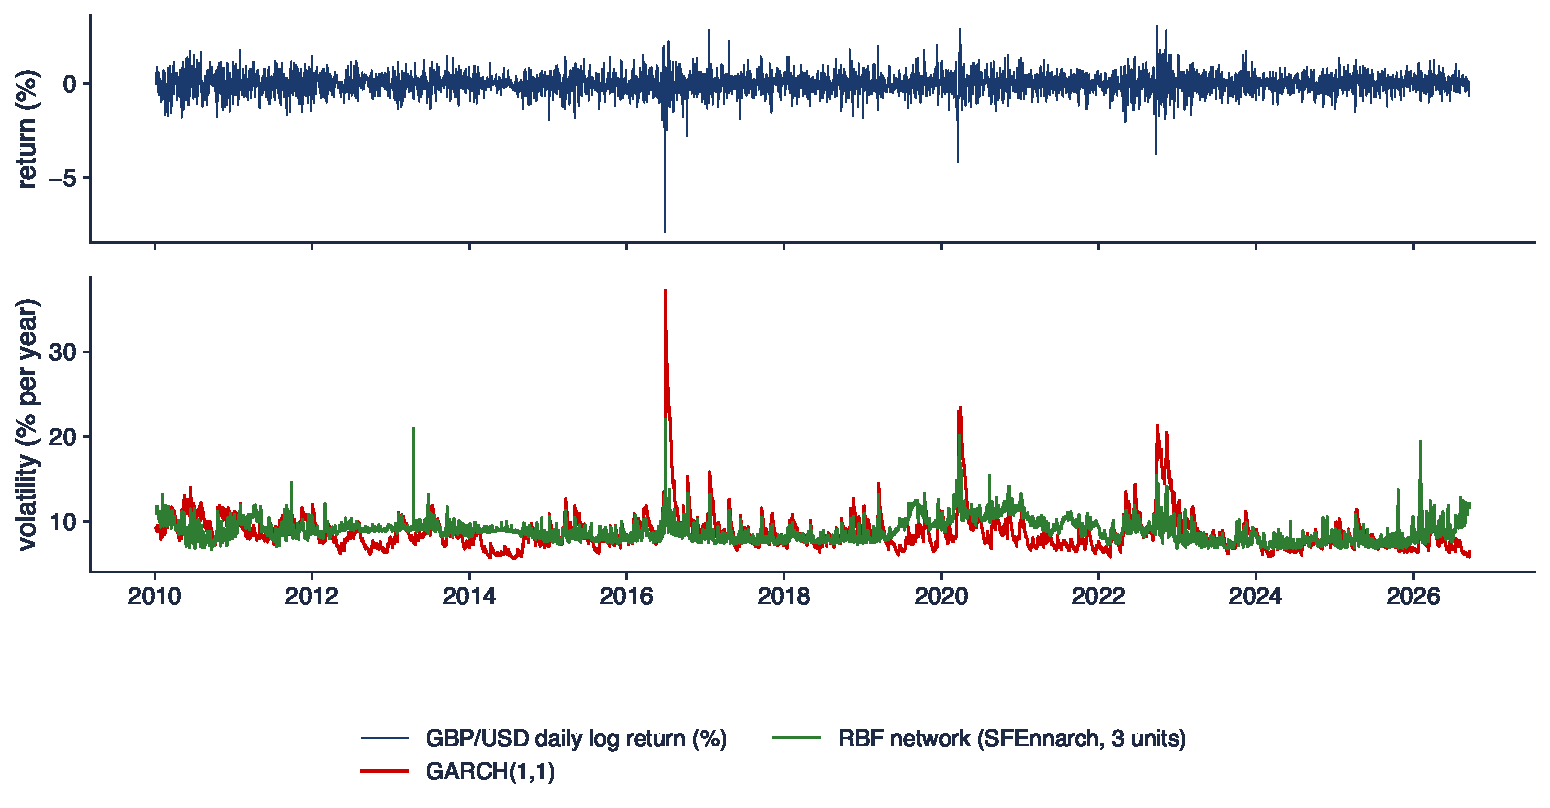
\includegraphics[width=0.97\textwidth,height=0.50\textheight,keepaspectratio]{sfm_ch13_nnarch.pdf}
\end{center}
\vspace{-0.25cm}
\begin{itemize}
    \item Daily data from 7 January 2010 (4\,048 days); annualised volatility of the RBF network and of GARCH(1,1) ($\hat\alpha = 0.077$, $\hat\beta = 0.892$)
    \item Average volatility: network 8.9\%, GARCH 8.8\%; correlation of the two paths $0.45$ (a small MLP: $0.43$)
\end{itemize}
\sfmquantlet{Ch_13}{SFM_ch13_neural_networks}
\end{frame}

\begin{frame}{Interpretation: Flexible Shape, Short Memory}
\itemsize{\small}
\begin{itemize}
    \item After the Brexit vote, GARCH peaks at 37.3\% (28 June 2016); the network only at 22.0\%
    \begin{itemize}
        \item the network sees only the last 3 returns: one large return raises its variance for 3 days, then the effect is gone
        \item GARCH(1,1) (\sfmchlink{https://danpele.github.io/SFM/EN/Courses/chapter9_arch_garch_models.pdf}{Chapter 9}): $\sigma_t^2 = \omega + \alpha\,r_{t-1}^2 + \beta\,\sigma_{t-1}^2$, with $\sigma_{t-1}^2$ yesterday's conditional variance
        \item the term $\beta\,\sigma_{t-1}^2$ carries the whole past: volatility clustering needs memory, not only flexibility
    \end{itemize}
    \item The mean network explains $0.08\%$ of the returns in sample: exchange rates are close to a random walk
    \begin{itemize}
        \item the useful part of NN-ARCH is the variance, as for GARCH
    \end{itemize}
    \item Lesson: good features (HAR averages, Section 7) matter more than the type of network
\end{itemize}
\end{frame}

\begin{frame}{Forecasting an Exchange Rate Level: SFEnnjpyusd}
\itemsize{\small}
\begin{itemize}
    \item The Quantlet \refSFEb{} forecasts the yen--dollar rate from its last 3 values with an RBF network of 3 units
    \begin{itemize}
        \item first 80\% of the days for training, last 20\% for testing; here USD/JPY from 2000, split on 21 June 2021
    \end{itemize}
    \item Two traps of level forecasting
    \begin{itemize}
        \item a level series looks predictable because $P_t \approx P_{t-1}$: the right benchmark is the random walk $\hat P_t = P_{t-1}$ (\sfmchlink{https://danpele.github.io/SFM/EN/Courses/chapter7_efficient_markets_random_walk_vr.pdf}{Chapter 7})
        \item a network with bounded units cannot extrapolate: the test levels go up to 163.9, the training maximum was 134.9
    \end{itemize}
    \item The original code rescales the test forecasts with the range of the test series, which is unknown in real time; here the training range is used
\end{itemize}
\end{frame}

\begin{frame}{The RBF Network against the Random Walk}
\itemsize{\footnotesize}
\begin{center}
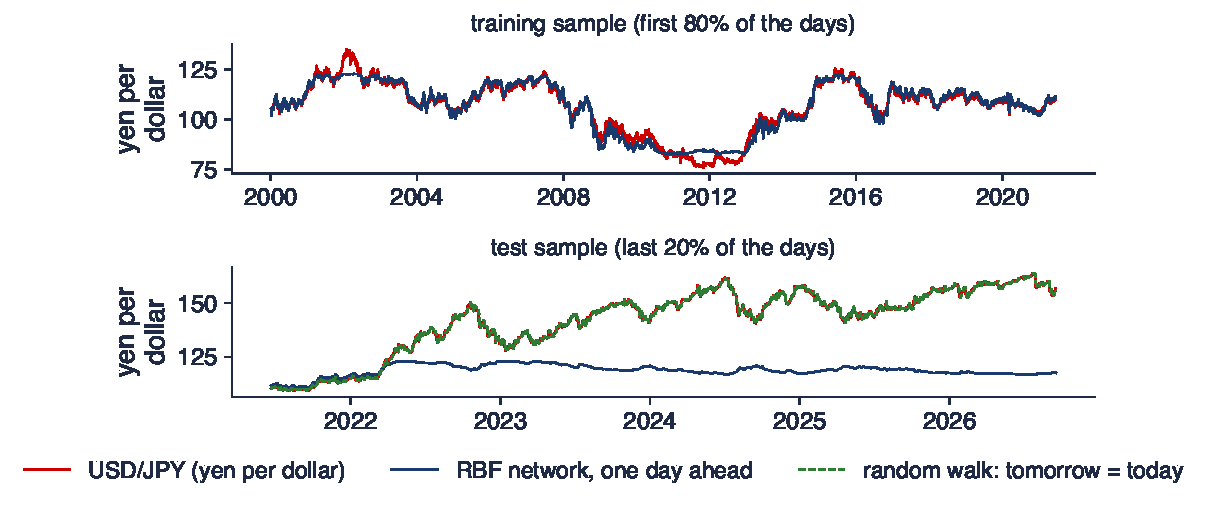
\includegraphics[width=0.97\textwidth,height=0.50\textheight,keepaspectratio]{sfm_ch13_nnjpy.pdf}
\end{center}
\vspace{-0.25cm}
\begin{itemize}
    \item RMSE (root mean squared error) in yen: training: network 2.64, random walk 0.66; test: network 27.56, random walk 0.89
    \item Interpretation: out of sample the network is 31 times worse than ``tomorrow = today''; on returns the same network has an out-of-sample $R^2$ of $-0.14\%$
\end{itemize}
\sfmquantlet{Ch_13}{SFM_ch13_neural_networks}
\end{frame}

\begin{frame}{Recap: Neural Networks}
\itemsize{\small}
\begin{itemize}
    \item An MLP is a linear model in learned nonlinear features; trained by gradient descent and back-propagation
    \item NN-ARCH: a flexible variance function, but without the memory of GARCH and without positivity
    \item Forecast returns, not levels, and always compare with the random walk
\end{itemize}
\end{frame}


%=============================================================================
\section{Application: Forecasting Realised Volatility}
%=============================================================================

\begin{frame}{Target and Features (1/2)}
\itemsize{\small}
\begin{itemize}
    \item Daily variance proxy of \sfmchlink{https://danpele.github.io/SFM/EN/Courses/chapter8_volatility_estimators.pdf}{Chapter 8} (no intraday data): an estimate of the variance of day $t$ from its open, high, low and close \[ v_t = o_t^2 + \tfrac12(u_t - d_t)^2 - (2\ln 2 - 1)c_t^2 \]
    \begin{itemize}
        \item $o_t$: the overnight log return (from the previous close to the open)
        \item $u_t, d_t, c_t$: log high, low and close relative to the open (the Garman--Klass term, \refGK)
    \end{itemize}
    \item \textbf{Target}: $y_t = \ln\big(\tfrac15\sum_{j=1}^{5} v_{t+j}\big)$, the log realised variance of the next week
    \begin{itemize}
        \item $j = 1, \dots, 5$: the next five trading days; the target is known only at the close of day $t + 5$
        \item logs make the target closer to Normal and the forecasts positive after $\exp$
    \end{itemize}
\end{itemize}
\end{frame}

\begin{frame}{Target and Features (2/2)}
\itemsize{\small}
\begin{itemize}
    \item \textbf{Features} at the close of day $t$
    \begin{itemize}
        \item HAR: $\ln v_t$, $\ln$ of the mean over 5 days (week) and over 22 days (month)
        \item extended (11): plus 4 lags of $\ln v_t$ ($\ln v_{t-1}, \dots, \ln v_{t-4}$), the 66-day mean, $r_t$, $\min(r_t, 0)$, $|r_t|$
    \end{itemize}
    \item Notation
    \begin{itemize}
        \item $r_t$: the log return of day $t$; $|r_t|$: its absolute value
        \item $\min(r_t, 0)$: the return if negative, 0 otherwise; it lets falls and rises act differently (the leverage effect)
    \end{itemize}
\end{itemize}
\end{frame}

\begin{frame}{The HAR Benchmark (1/2)}
\itemsize{\small}
\begin{itemize}
    \item \textbf{HAR} (heterogeneous autoregressive) model \refCorsi{} \[ y_t = \beta_0 + \beta_d\ln v_t + \beta_w\ln v_t^{(w)} + \beta_m\ln v_t^{(m)} + u_t \]
    \begin{itemize}
        \item $v_t^{(w)}$, $v_t^{(m)}$: the mean of $v$ over the last 5 days (week) and over the last 22 days (month)
        \item $\beta_0$: the constant; $\beta_d, \beta_w, \beta_m$: the weights of the three horizons; $u_t$: the error
    \end{itemize}
    \item Interpretation
    \begin{itemize}
        \item three horizons of traders (daily, weekly, monthly); estimated by OLS
        \item with positive weights on the three horizons, a shock to volatility fades slowly
        \item a simple linear model that mimics long memory (\sfmchlink{https://danpele.github.io/SFM/EN/Courses/chapter11_fractal_markets_long_memory.pdf}{Chapter 11}) and is hard to beat
    \end{itemize}
\end{itemize}
\end{frame}

\begin{frame}{The HAR Benchmark (2/2)}
\itemsize{\small}
\begin{itemize}
    \item The question of this section
    \begin{itemize}
        \item do lasso, random forest, gradient boosting or an MLP add anything to HAR out of sample?
        \item a large study with intraday data finds modest gains, mainly from extra features \refCSV
    \end{itemize}
    \item Design: walk-forward of Section 3, yearly refits; S\&P 500 from 2013, Bitcoin from 2018
    \begin{itemize}
        \item variance forecast $\hat h_t = \exp(\hat y_t + \hat s^2/2)$, $\hat s^2$ the residual variance in training (the log-Normal mean)
        \item $\hat y_t$: the forecast of the log variance; $\exp(\hat y_t)$ alone would underestimate the mean variance, hence the term $\hat s^2/2$
    \end{itemize}
\end{itemize}
\end{frame}

\begin{frame}{Evaluation (1/3): Out-of-Sample $R^2$}
\itemsize{\small}
\begin{itemize}
    \item \textbf{Out-of-sample} $R^2$ against a benchmark forecast $\tilde y_t$ \refCT{} \[ R^2_{OOS} = 1 - \frac{\sum_t (y_t - \hat y_t)^2}{\sum_t (y_t - \tilde y_t)^2} \]
    \begin{itemize}
        \item $\hat y_t$: the forecast of the model; sums over the test days only
        \item benchmark $\tilde y_t$: the training mean, or HAR
    \end{itemize}
    \item Reading
    \begin{itemize}
        \item $R^2_{OOS} \le 1$; $R^2_{OOS} > 0$: smaller squared error than the benchmark; $R^2_{OOS} < 0$: worse than the benchmark
        \item unlike the in-sample $R^2$, it can be negative
    \end{itemize}
    \item Step by step, S\&P 500, MLP against HAR
    \begin{itemize}
        \item $1 - 0.397/0.433 = 1 - 0.917$, i.e.\ $+8.3\%$
    \end{itemize}
\end{itemize}
\end{frame}

\begin{frame}{Evaluation (2/3): QLIKE}
\itemsize{\small}
\begin{itemize}
    \item \textbf{QLIKE} (\sfmchlink{https://danpele.github.io/SFM/EN/Courses/chapter8_volatility_estimators.pdf}{Chapter 8}): a loss for variance forecasts, robust to a noisy proxy \refPatton{} \[ L_t = \frac{\mathrm{RV}_t}{\hat h_t} + \ln\hat h_t \]
    \begin{itemize}
        \item $\mathrm{RV}_t$: the realised variance of the next 5 days (the target, in levels); $\hat h_t$: its forecast
        \item for a given $\mathrm{RV}_t$, the loss is smallest at $\hat h_t = \mathrm{RV}_t$; lower average QLIKE is better
    \end{itemize}
    \item Asymmetry
    \begin{itemize}
        \item for $\mathrm{RV} = 1$: $\hat h = 0.5$ costs $1.307$, $\hat h = 2$ costs $1.193$
        \item under-prediction is punished more: for risk management, underestimating volatility is the costly error
    \end{itemize}
\end{itemize}
\end{frame}

\begin{frame}{Evaluation (3/3): the Diebold--Mariano Test}
\itemsize{\small}
\begin{itemize}
    \item \textbf{Diebold--Mariano} test \refDM: do two models $A$ and $B$ have the same expected loss? \[ d_t = L_t^{A} - L_t^{B}, \qquad \mathrm{DM} = \frac{\bar d}{\sqrt{\widehat{\mathrm{LRV}}/n}} \sim N(0,1) \text{ under equal accuracy} \]
    \begin{itemize}
        \item $L_t^{A}$, $L_t^{B}$: the losses of the two models on day $t$; $\bar d$: the mean of $d_t$; $n$: the number of test days
        \item $\widehat{\mathrm{LRV}}$: the Newey--West long-run variance of $d_t$ (5 lags), because overlapping targets make $d_t$ autocorrelated
    \end{itemize}
    \item Reading
    \begin{itemize}
        \item DM $< 0$: $A$ has the smaller loss; DM $> 0$: $B$ is better
        \item $|\mathrm{DM}| > 1.96$: the difference is significant at 5\%
    \end{itemize}
\end{itemize}
\end{frame}

\begin{frame}{Results: S\&P 500 and Bitcoin}
\itemsize{\footnotesize}
\begin{center}
\scriptsize
\begin{tabular}{llrrrr}
\toprule
& Model & $R^2_{OOS}$ vs.\ mean & $R^2_{OOS}$ vs.\ HAR & QLIKE & DM vs.\ HAR (p) \\
\midrule
S\&P 500 & HAR & $61.5$ & -- & $0.414$ & -- \\
 & Lasso & $64.2$ & ${+7.1}$ & $0.400$ & ${-5.12}$ ($<$\,0.001) \\
 & RF & $61.9$ & ${+1.0}$ & $0.416$ & ${+0.32}$ (0.747) \\
 & GB & $60.4$ & ${-2.7}$ & $0.421$ & ${+1.02}$ (0.308) \\
 & MLP & $64.7$ & ${+8.3}$ & $0.398$ & ${-3.96}$ ($<$\,0.001) \\
\midrule
Bitcoin & HAR & $44.0$ & -- & $3.111$ & -- \\
 & Lasso & $45.1$ & ${+2.0}$ & $3.108$ & ${-0.64}$ (0.520) \\
 & RF & $43.4$ & ${-1.2}$ & $3.119$ & ${+0.81}$ (0.418) \\
 & GB & $41.7$ & ${-4.2}$ & $3.148$ & ${+2.12}$ (0.034) \\
 & MLP & $43.8$ & ${-0.3}$ & $3.123$ & ${+1.10}$ (0.272) \\
\bottomrule
\end{tabular}
\end{center}
\begin{itemize}
    \item Forecasts for 3\,444 days (S\&P 500, from 2 January 2013) and 3\,178 days (Bitcoin, from 1 January 2018); $R^2_{OOS}$ in \%, on log RV; GB: gradient boosting
    \item S\&P 500: lasso and MLP beat HAR significantly ($+7.1\%$, $+8.3\%$); random forest and boosting do not
    \item Bitcoin: no model beats HAR; boosting is significantly worse (DM $+2.12$)
\end{itemize}\sfmquantlet{Ch_13}{SFM_ch13_volatility_forecast}
\end{frame}

\begin{frame}{Forecasts in Two Storms: 2020 and 2025}
\itemsize{\footnotesize}
\begin{center}
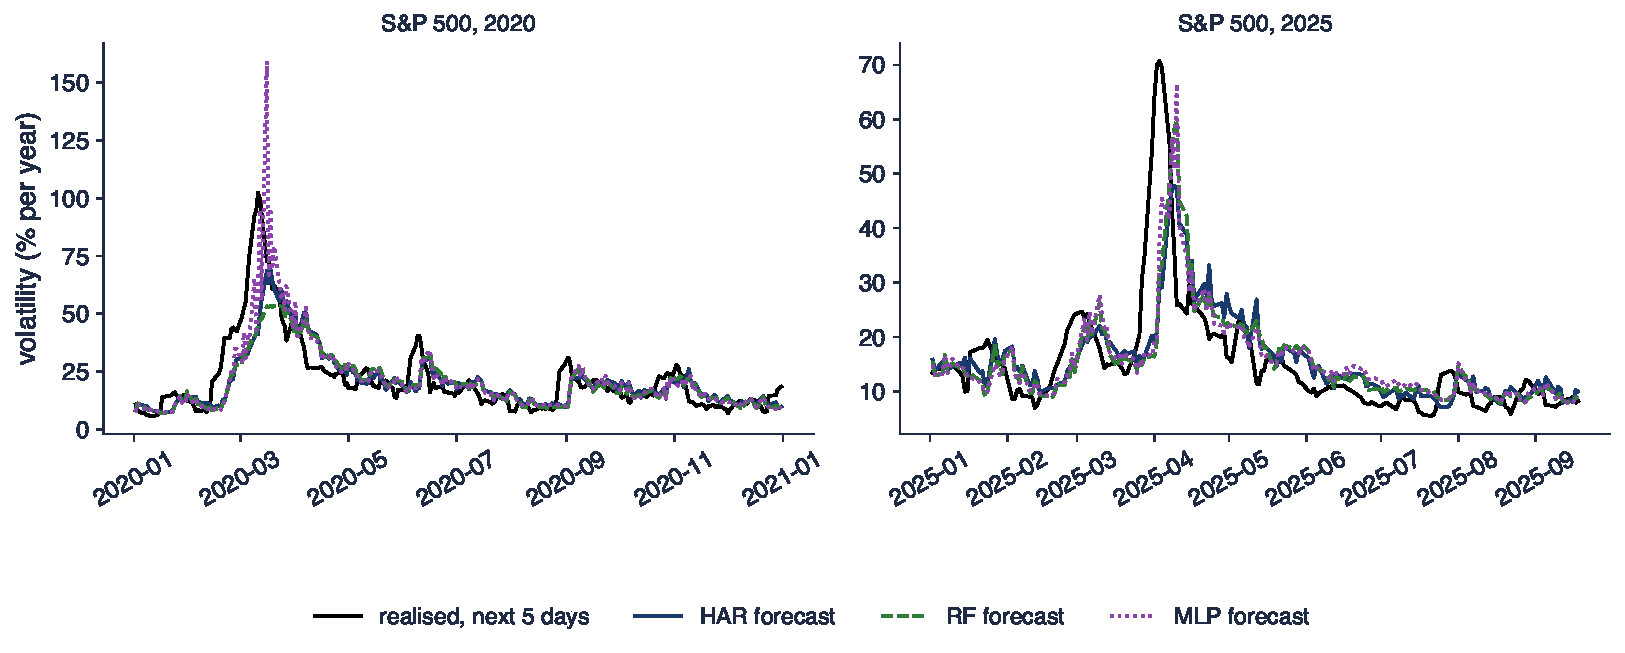
\includegraphics[width=0.97\textwidth,height=0.50\textheight,keepaspectratio]{sfm_ch13_rv_forecasts.pdf}
\end{center}
\vspace{-0.25cm}
\begin{itemize}
    \item S\&P 500: annualised realised volatility of the next 5 days, $\sqrt{252\,\mathrm{RV}_t}$, and the HAR, random forest and MLP forecasts made at the close of day $t$
    \item Interpretation: all models react only after the first shock (March 2020, April 2025); the forest is capped by the largest values it saw in training, the MLP can overshoot
\end{itemize}
\sfmquantlet{Ch_13}{SFM_ch13_volatility_forecast}
\end{frame}

\begin{frame}{Feature Importance: Permutation and Shapley Values}
\itemsize{\small}
\begin{itemize}
    \item \textbf{Permutation importance}: shuffle one feature in the test data and measure how much the test MSE rises
    \begin{itemize}
        \item large increase: the model relies on the feature; correlated features share (and hide) their importance
    \end{itemize}
    \item \textbf{Shapley values} (game theory): $\hat f(x) = \phi_0 + \sum_j \phi_j(x)$, $\phi_j$ the fair share of feature $j$ in the forecast
    \begin{itemize}
        \item $\phi_0$: the average forecast; $\phi_j(x) > 0$: feature $j$ raises this forecast above the average, $\phi_j(x) < 0$: lowers it
        \item $\phi_j$ averages the change of $\hat f$ when $j$ joins every subset of the other features
        \item SHAP (Shapley additive explanations) \refLL: fast versions for trees; for a linear model $\phi_j = \beta_j(x_j - \bar x_j)$
    \end{itemize}
    \item Both describe the model, not the economy: importance is not causality
\end{itemize}
\end{frame}

\begin{frame}{The Features Used by the Forest}
\itemsize{\footnotesize}
\begin{center}
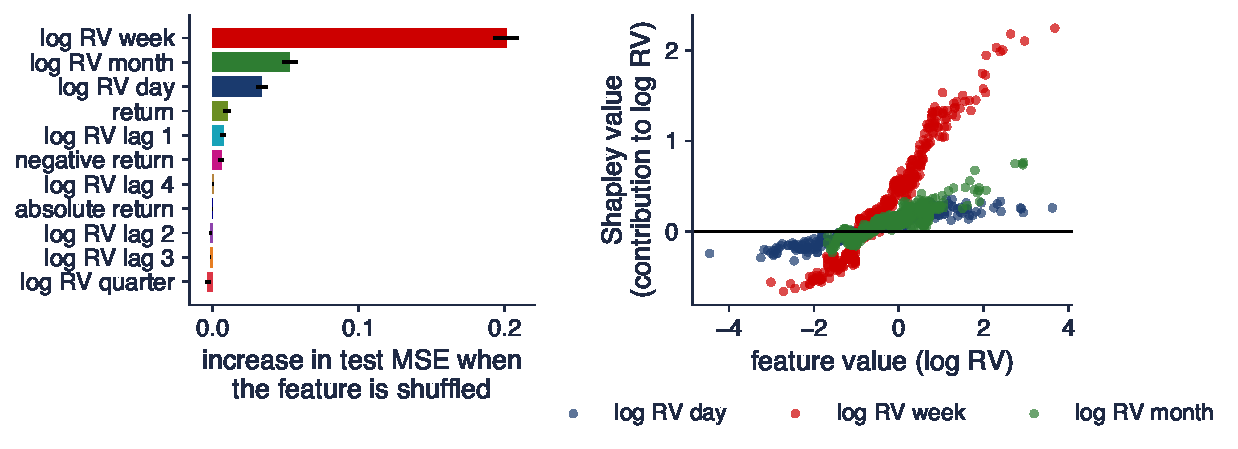
\includegraphics[width=0.97\textwidth,height=0.48\textheight,keepaspectratio]{sfm_ch13_importance.pdf}
\end{center}
\vspace{-0.25cm}
\begin{itemize}
    \item Left: random forest on 11 features, trained to 2019, tested 2020--2026 (1\,682 days): shuffling the weekly variance raises the MSE by $0.201$, the monthly by $0.053$, the daily by $0.034$
    \item Right: exact Shapley values of a forest on the 3 HAR features; mean $|\phi|$: week $0.52$, month $0.13$, day $0.13$; the effect is nonlinear and grows with the level of volatility
\end{itemize}
\sfmquantlet{Ch_13}{SFM_ch13_volatility_forecast}
\end{frame}

\begin{frame}{Recap: Forecasting Realised Volatility}
\itemsize{\small}
\begin{itemize}
    \item HAR is a strong benchmark; penalised and neural models add a few per cent on the S\&P 500, nothing on Bitcoin
    \item Evaluate with out-of-sample $R^2$, QLIKE and Diebold--Mariano, on a walk-forward design
    \item The weekly variance carries most of the information; importance measures describe the model, not causes
\end{itemize}
\end{frame}


%=============================================================================
\section{Application: the Sign of Tomorrow's Return}
%=============================================================================

\begin{frame}{A Classification Problem}
\itemsize{\small}
\begin{itemize}
    \item Target: $y_t = \mathbf{1}\{r_{t+1} > 0\}$; features at the close of day $t$: the last 5 returns, sums over 5, 21 and 63 days, volatility over 21 and 63 days
    \begin{itemize}
        \item $\mathbf{1}\{\cdot\}$: the indicator, 1 if the condition holds and 0 otherwise; $y_t = 1$: tomorrow's return is positive
        \item models: logit (\sfmchlink{https://danpele.github.io/SFM/EN/Courses/chapter12_scoring_models.pdf}{Chapter 12}), random forest and gradient boosting classifiers; walk-forward, yearly refits
        \item S\&P 500 and BET from 2008, Bitcoin from 2018
    \end{itemize}
    \item Metrics (defined in \sfmchlink{https://danpele.github.io/SFM/EN/Courses/chapter12_scoring_models.pdf}{Chapter 12})
    \begin{itemize}
        \item accuracy: the share of days with the right sign; AUC (area under the ROC curve): 0.5 means no ranking skill
    \end{itemize}
    \item Why expect little: weak-form efficiency (\sfmchlink{https://danpele.github.io/SFM/EN/Courses/chapter7_efficient_markets_random_walk_vr.pdf}{Chapter 7})
    \begin{itemize}
        \item any reliable pattern in past returns would be traded away
    \end{itemize}
\end{itemize}
\end{frame}

\begin{frame}{The Right Baseline}
\itemsize{\small}
\begin{itemize}
    \item \textbf{Majority-class baseline}: always forecast the more frequent class of the training sample (here: ``up'')
    \begin{itemize}
        \item S\&P 500 since 2008: 54.4\% of the days are up, so ``always up'' is right on 54.4\% of the days
        \item an accuracy of 53\% sounds like skill; against this baseline it is a loss
    \end{itemize}
    \item Test against the baseline: $z = (\widehat{\mathrm{acc}} - \mathrm{acc}_0)/\sqrt{\mathrm{acc}_0(1 - \mathrm{acc}_0)/n}$
    \begin{itemize}
        \item $\widehat{\mathrm{acc}}$: the accuracy of the model; $\mathrm{acc}_0$: that of the baseline; $n$: the test days; $z \approx N(0,1)$ if the model has no extra skill
        \item S\&P 500, $n = 4\,705$: standard error 0.73 points; a 95\% band of $\pm$1.4 points around the baseline
        \item random forest: 53.1\%, $z = -1.79$ (p 0.074); boosting: 52.1\%, $z = -3.19$ (p 0.001)
    \end{itemize}
    \item For returns, the matching baseline is the zero or historical-mean forecast \refWG
\end{itemize}
\end{frame}

\begin{frame}{Accuracy against the Baseline}
\itemsize{\footnotesize}
\begin{center}
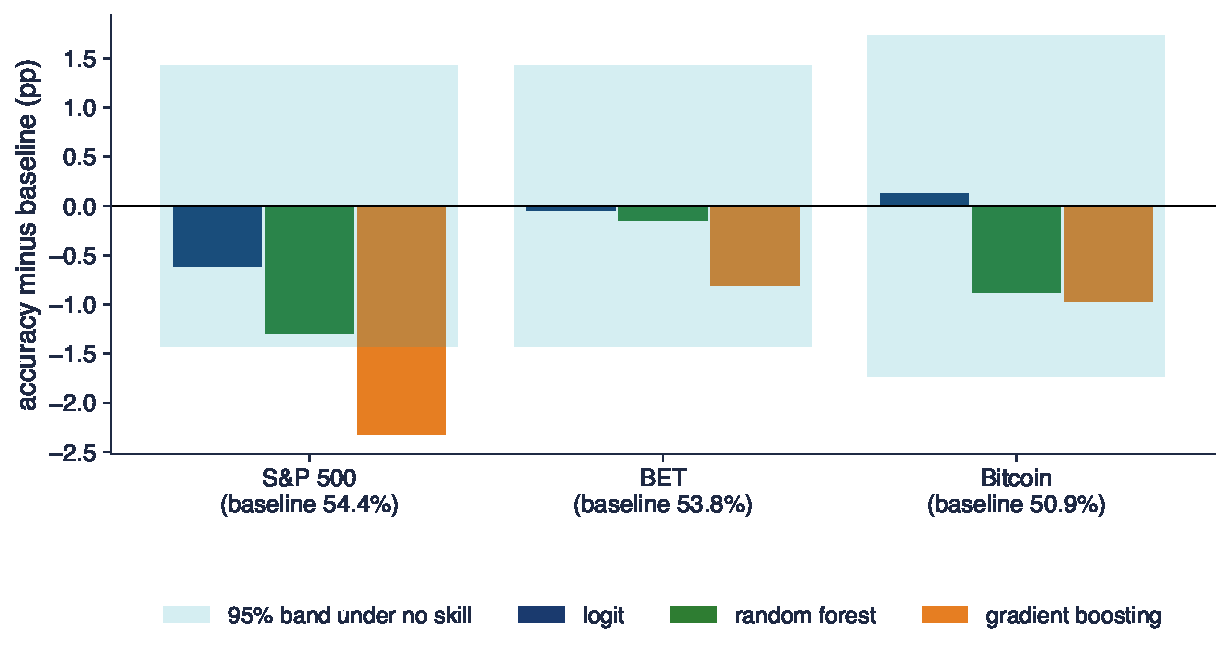
\includegraphics[width=0.97\textwidth,height=0.48\textheight,keepaspectratio]{sfm_ch13_sign.pdf}
\end{center}
\vspace{-0.25cm}
\begin{itemize}
    \item Accuracy minus the baseline accuracy (percentage points); band: $\pm 1.96$ standard errors around zero
    \item AUC of the logit and of the forest: S\&P 500 0.511 and 0.507, BET 0.533 and 0.533, Bitcoin 0.515 and 0.519; logit forecasts ``up'' on 86\% of S\&P 500 days
\end{itemize}
\sfmquantlet{Ch_13}{SFM_ch13_sign_prediction}
\end{frame}

\begin{frame}{Interpretation: Why Sign Prediction Mostly Fails}
\itemsize{\small}
\begin{itemize}
    \item No model beats ``always up'' significantly on any market; the flexible models do worse than the logit
    \begin{itemize}
        \item S\&P 500: logit $-0.6$, forest $-1.3$, boosting $-2.3$ points; Bitcoin: logit $+0.1$, forest $-0.9$
    \end{itemize}
    \item The signal-to-noise ratio of daily returns is tiny
    \begin{itemize}
        \item flexible models find patterns in the noise of the training years (Section 2); the logit is close to the baseline because it hardly moves
    \end{itemize}
    \item Even a real edge of one point would rarely survive costs: a daily sign strategy trades very often
    \begin{itemize}
        \item ML gains in returns come from large cross-sections at monthly horizons, not from one index tomorrow (Section 11)
    \end{itemize}
\end{itemize}
\end{frame}

\begin{frame}{Recap: The Sign of Tomorrow's Return}
\itemsize{\small}
\begin{itemize}
    \item Always compare accuracy with the majority-class baseline, and test the difference
    \item On the S\&P 500, BET and Bitcoin no model beats ``always up'' significantly
    \item Weak-form efficiency (\sfmchlink{https://danpele.github.io/SFM/EN/Courses/chapter7_efficient_markets_random_walk_vr.pdf}{Chapter 7}) predicts this result
\end{itemize}
\end{frame}


%=============================================================================
\section{Application: VaR 1\% by Quantile Methods}
%=============================================================================

\begin{frame}{Quantile Regression (1/2)}
\itemsize{\small}
\begin{itemize}
    \item \refKB: estimate the conditional $\alpha$-quantile $q_\alpha(x) = x^\top\beta_\alpha$ by minimising the \textbf{quantile (pinball) loss}
    \begin{itemize}
        \item $q_\alpha(x)$: the level below which $y$ falls with probability $\alpha$, given $x$; $\beta_\alpha$: coefficients specific to the level $\alpha$
    \end{itemize}
    \item The loss of an error $u = y - q$: \[ \rho_\alpha(u) = u\,(\alpha - \mathbf{1}\{u < 0\}) \]
    \begin{itemize}
        \item below the quantile ($u < 0$) the error costs $(1 - \alpha)|u|$, above it $\alpha|u|$
        \item with $\alpha = 0.01$, the minimum is reached when about 1\% of the observations lie below $q$
    \end{itemize}
\end{itemize}
\end{frame}

\begin{frame}{Quantile Regression (2/2)}
\itemsize{\small}
\begin{itemize}
    \item With $\alpha = 0.01$ and $q = -\mathrm{VaR}$: the average quantile loss of \sfmchlink{https://danpele.github.io/SFM/EN/Courses/chapter10_var_es_backtesting.pdf}{Chapter 10}
    \begin{itemize}
        \item $(\alpha - I_t)(r_t + \mathrm{VaR}_t)$, with $I_t = 1$ if $r_t < -\mathrm{VaR}_t$ (an exception) and 0 otherwise
    \end{itemize}
    \item VaR 1\% for day $t + 1$: $\widehat{\mathrm{VaR}}_t = -\hat q_{0.01}(x_t)$, with $x_t$ = daily, weekly and monthly volatility (square roots of the proxy) and $r_t$
    \begin{itemize}
        \item no distribution is assumed: the data choose how volatility maps into the tail; CAViaR \refCAViaR{} is a dynamic version
    \end{itemize}
    \item \textbf{Quantile gradient boosting}: the same loss with boosted trees (Section 5)
    \begin{itemize}
        \item flexible, but at 1\% each leaf sees few tail observations: high variance
    \end{itemize}
\end{itemize}
\end{frame}

\begin{frame}{Backtest of VaR 1\%: Quantile Methods, HS and GARCH-t (1/2)}
\itemsize{\footnotesize}
\begin{center}
\scriptsize
\begin{tabular}{llrrrrrr}
\toprule
& Method & $x$ & rate (\%) & p Kupiec & p ind. & loss $\times 100$ & mean VaR \\
\midrule
S\&P 500 & QR & 28 & $0.81$ & 0.252 & 0.020 & $3.38$ & $2.70$ \\
 & QGB & 42 & $1.22$ & 0.213 & 0.015 & $3.51$ & $2.46$ \\
 & HS & 46 & $1.33$ & 0.061 & $<$\,0.001 & $4.78$ & $2.97$ \\
 & GARCH-t & 52 & $1.51$ & 0.005 & 0.008 & $3.50$ & $2.42$ \\
\midrule
Bitcoin & QR & 23 & $0.72$ & 0.098 & 0.563 & $13.03$ & $10.46$ \\
 & QGB & 47 & $1.48$ & 0.012 & 0.235 & $13.19$ & $8.86$ \\
 & HS & 32 & $1.01$ & 0.974 & 0.332 & $13.01$ & $9.30$ \\
 & GARCH-t & 41 & $1.29$ & 0.117 & 0.558 & $13.15$ & $8.52$ \\
\bottomrule
\end{tabular}
\end{center}
\begin{itemize}
    \item Columns
    \begin{itemize}
        \item $x$: the number of exceptions ($r_{t+1} < -\widehat{\mathrm{VaR}}_t$) in $n$ test days; rate $= x/n$, target 1\%
        \item p Kupiec: p-value of the Kupiec test of the rate; p ind.: p-value of the Christoffersen test of independence (\sfmchlink{https://danpele.github.io/SFM/EN/Courses/chapter10_var_es_backtesting.pdf}{Chapter 10})
        \item loss $\times 100$: the mean quantile loss (smaller is better); mean VaR: the average VaR 1\%, in \%
    \end{itemize}
    \item Methods
    \begin{itemize}
        \item QR: linear quantile regression; QGB: quantile gradient boosting
        \item HS: historical simulation on 500 days; GARCH-t: re-estimated each January (\sfmchlink{https://danpele.github.io/SFM/EN/Courses/chapter10_var_es_backtesting.pdf}{Chapter 10})
    \end{itemize}
\end{itemize}\sfmquantlet{Ch_13}{SFM_ch13_quantile_var}
\end{frame}

\begin{frame}{Backtest of VaR 1\%: Quantile Methods, HS and GARCH-t (2/2)}
\itemsize{\footnotesize}
\begin{itemize}
    \item S\&P 500 (3\,448 days from 2 January 2013): QR has the right rate (0.81\%) and the smallest loss
    \begin{itemize}
        \item its exceptions are not fully independent (p ind.\ 0.020)
        \item GARCH-t is exceeded too often (1.51\%)
    \end{itemize}
    \item Bitcoin (3\,182 days): HS has the best rate (1.01\%)
    \begin{itemize}
        \item QGB is rejected by the Kupiec test (1.48\%, p 0.012)
        \item at 1\% each leaf of the boosted trees sees few tail days: high variance (Section 2)
    \end{itemize}
    \item Reading the p-values
    \begin{itemize}
        \item p Kupiec below 0.05: the exception rate differs significantly from 1\%
        \item p ind.\ below 0.05: the exceptions come in clusters, so the VaR reacts too slowly
    \end{itemize}
\end{itemize}
\end{frame}

\begin{frame}{VaR 1\% Forecasts in 2020 and 2025}
\itemsize{\footnotesize}
\begin{center}
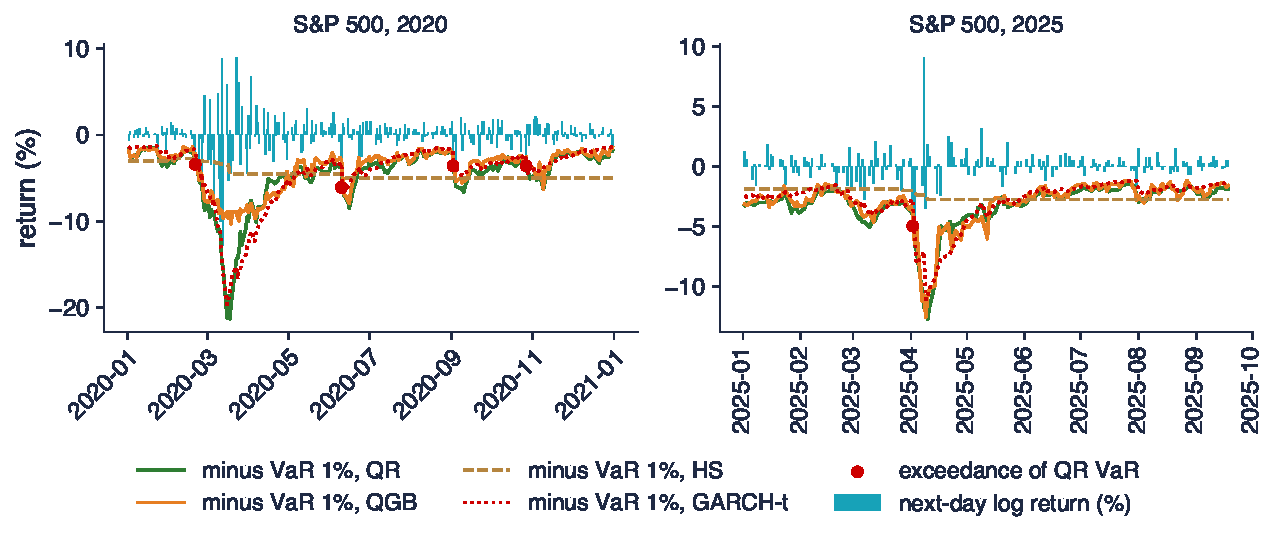
\includegraphics[width=0.97\textwidth,height=0.48\textheight,keepaspectratio]{sfm_ch13_qvar.pdf}
\end{center}
\vspace{-0.25cm}
\begin{itemize}
    \item S\&P 500: next-day returns and minus VaR 1\% of the four methods; dots: exceedances of the quantile-regression VaR
    \item Interpretation: QR and GARCH-t move with volatility; HS reacts only slowly; in 2020 HS was exceeded 10 times, QR 4 times, and the HS exceptions cluster (p ind.\ $<$\,0.001)
\end{itemize}
\sfmquantlet{Ch_13}{SFM_ch13_quantile_var}
\end{frame}

\begin{frame}{Recap: VaR 1\% by Quantile Methods}
\itemsize{\small}
\begin{itemize}
    \item Quantile regression minimises the pinball loss: VaR without a distributional assumption
    \item A linear quantile model on volatility features passes the Kupiec test for the S\&P 500
    \item Flexible quantile models at 1\% need much more tail data than we have
\end{itemize}
\end{frame}


%=============================================================================
\section{Data Snooping and the Deflated Sharpe Ratio}
%=============================================================================

\begin{frame}{The Best of $N$ Strategies (1/2)}
\itemsize{\small}
\begin{itemize}
    \item \textbf{Data snooping}: trying many models or rules on the same data and reporting the best \refWhite
    \begin{itemize}
        \item with enough trials, a rule without skill looks excellent in sample
        \item hundreds of published return predictors would not survive a multiple-testing correction \refHLZ
    \end{itemize}
    \item The annual Sharpe ratio of a strategy without skill over $Y$ years is about $N(0, 1/Y)$
    \begin{itemize}
        \item Sharpe ratio: mean excess return divided by its standard deviation (\sfmchlink{https://danpele.github.io/SFM/EN/Courses/chapter1_data_returns_indicators.pdf}{Chapter 1}); $Y$: the number of years of data
        \item mean 0: no skill; variance $1/Y$: the estimation error, which falls with the length of the sample
    \end{itemize}
\end{itemize}
\end{frame}

\begin{frame}{The Best of $N$ Strategies (2/2)}
\itemsize{\small}
\begin{itemize}
    \item Expected maximum of $N$ independent zero-skill trials \refBLdP{} \[ \mathrm{E}[\max] \approx \sigma\Big[(1 - \gamma)\,\Phi^{-1}\big(1 - \tfrac1N\big) + \gamma\,\Phi^{-1}\big(1 - \tfrac{1}{Ne}\big)\Big] \]
    \begin{itemize}
        \item $\sigma$: the standard deviation of the Sharpe ratios across trials ($1/\sqrt{Y}$ above); $N$: the number of trials
        \item $\Phi^{-1}$: the quantile function of the standard Normal distribution; $e \approx 2.718$; $\gamma = 0.5772$: the Euler--Mascheroni constant
    \end{itemize}
    \item Example: 10 years, $\sigma = 1/\sqrt{10} = 0.316$, $N = 100$
    \begin{itemize}
        \item $0.316\,[(1 - \gamma)\,2.326 + \gamma\,2.680] = 0.80$: a Sharpe ratio this large is expected from pure luck
        \item simulation: the best of 10, 100 and 1000 zero-skill strategies has an average Sharpe ratio of $0.48$, $0.79$, $1.02$
    \end{itemize}
\end{itemize}
\end{frame}

\begin{frame}{Selection Bias in Practice}
\itemsize{\footnotesize}
\begin{center}
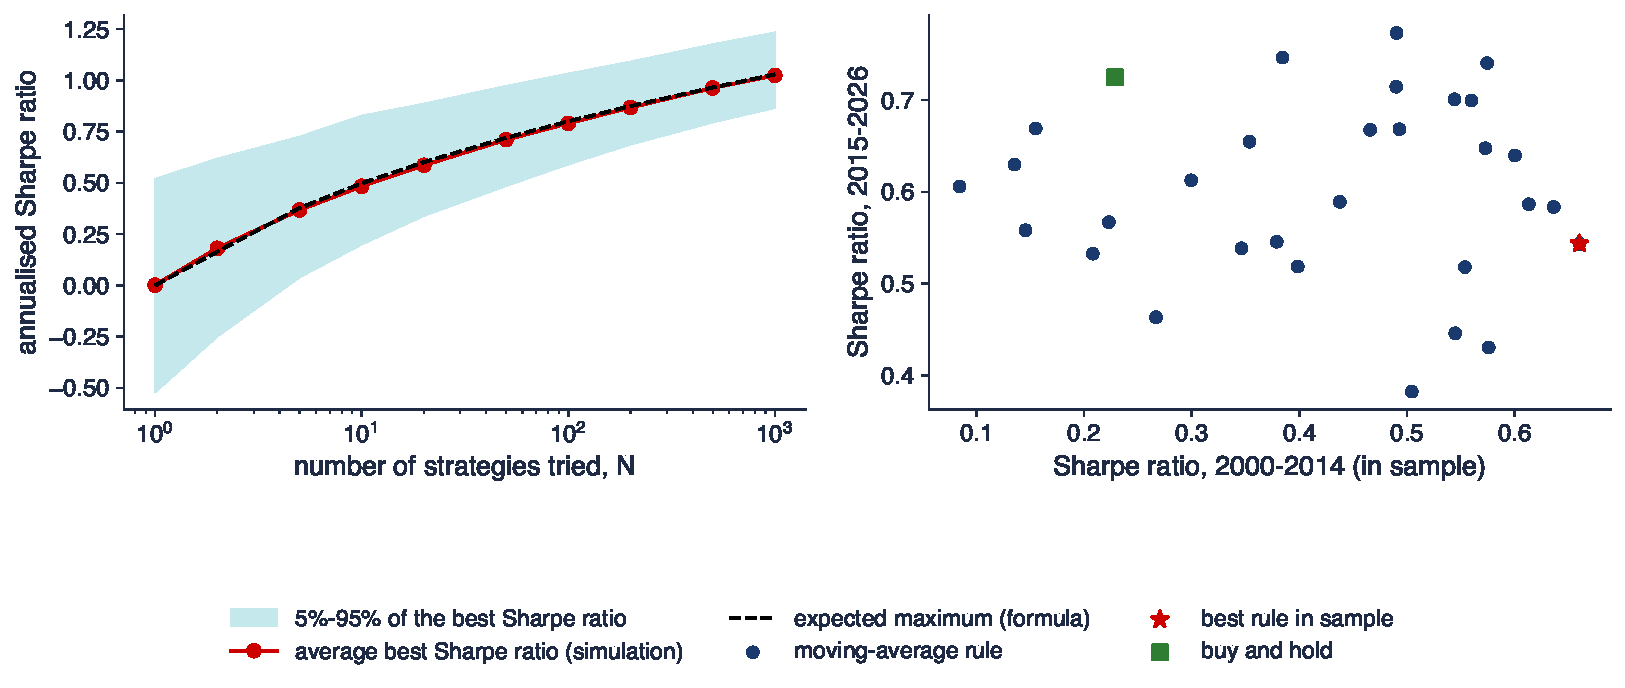
\includegraphics[width=0.97\textwidth,height=0.48\textheight,keepaspectratio]{sfm_ch13_snooping.pdf}
\end{center}
\vspace{-0.25cm}
\begin{itemize}
    \item Left: the best annual Sharpe ratio among $N$ strategies without skill (10 years); right: 30 moving-average rules on the S\&P 500 (long or cash), 2000--2014 against 2015--2026
    \item Interpretation: the best rule in sample (MA 50/200, Sharpe $0.66$) earns $0.54$ afterwards, rank 22 of 30, below buy and hold ($0.72$); in and out of sample Sharpe ratios correlate $0.04$
\end{itemize}
\sfmquantlet{Ch_13}{SFM_ch13_data_snooping}
\end{frame}

\begin{frame}{The Deflated Sharpe Ratio (1/2)}
\itemsize{\small}
\begin{itemize}
    \item \refBLdP: the probability that the true Sharpe ratio exceeds what the best of $N$ trials would show by luck \[ \mathrm{DSR} = \Phi\Big(\dfrac{(\widehat{SR} - SR_0)\sqrt{T - 1}}{\sqrt{1 - \hat\gamma_3\widehat{SR} + \frac{\hat\gamma_4 - 1}{4}\widehat{SR}^2}}\Big) \]
    \item Notation
    \begin{itemize}
        \item $\widehat{SR}$: the per-day Sharpe ratio of the chosen strategy; $T$: the number of days
        \item $SR_0$: the expected maximum of $N$ zero-skill trials (above), with $\sigma$ = the standard deviation of the $N$ Sharpe ratios tried
        \item $\hat\gamma_3$: the skewness, $\hat\gamma_4$: the kurtosis of the daily returns (3 for the Normal distribution); $\Phi$: the standard Normal distribution function
    \end{itemize}
    \item Reading
    \begin{itemize}
        \item the DSR is a probability in $(0, 1)$; above 0.95: the Sharpe ratio is significant after the correction for $N$ trials
        \item negative skewness and fat tails enlarge the denominator and lower the DSR
    \end{itemize}
\end{itemize}
\end{frame}

\begin{frame}{The Deflated Sharpe Ratio (2/2)}
\itemsize{\small}
\begin{itemize}
    \item \textbf{Step by step}: the best MA rule, $N = 30$, $T = 3\,769$ days
    \begin{itemize}
        \item $\widehat{SR} = 0.0416$ per day ($\times\sqrt{252} = 0.66$); $\hat\gamma_3 = -0.44$, $\hat\gamma_4 = 12.0$
        \item $SR_0 = 0.0105\,[(1 - \gamma)\,1.834 + \gamma\,2.249] = 0.0219$ (annual $0.35$)
        \item $z$, the argument of $\Phi$ in the DSR formula: $z = 1.20$, so DSR $= \Phi(z) = 0.88$
        \item without the correction for $N$ (PSR, probabilistic Sharpe ratio, $SR_0 = 0$): $0.994$
    \end{itemize}
    \item Interpretation: alone the rule looks significant; after 30 trials it is not (DSR below 0.95), as its later performance confirms
\end{itemize}
\end{frame}

\begin{frame}{Recap: Data Snooping}
\itemsize{\small}
\begin{itemize}
    \item The best of many trials is biased upwards; the bias grows like $\sqrt{2\ln N}$
    \item Report the number of trials and deflate the Sharpe ratio
    \item A final test sample used only once is the simplest protection
\end{itemize}
\end{frame}


%=============================================================================
\section{Case Study: Gu, Kelly and Xiu (2020)}
%=============================================================================

\begin{frame}{Empirical Asset Pricing via Machine Learning}
\itemsize{\footnotesize}
\begin{columns}[T]
\begin{column}{0.60\textwidth}
\begin{itemize}
    \item \refGKX: which methods best predict the monthly return of individual US stocks?
    \begin{itemize}
        \item nearly 30,000 stocks, 1957--2016; 94 firm characteristics, interacted with 8 macroeconomic variables, plus 74 industry dummies: 920 features
    \end{itemize}
    \item Design: 18 years of training (1957--1974), 12 of validation (1975--1986), 30 of test (1987--2016)
    \begin{itemize}
        \item refit once a year; the training window grows, the validation window rolls forward: a walk-forward design
        \item models: OLS, penalised and dimension-reduction regressions, random forest, boosted trees
        \item networks NN1--NN5: NN$k$ has $k$ hidden layers
    \end{itemize}
\end{itemize}
\end{column}
\begin{column}{0.36\textwidth}
\centering
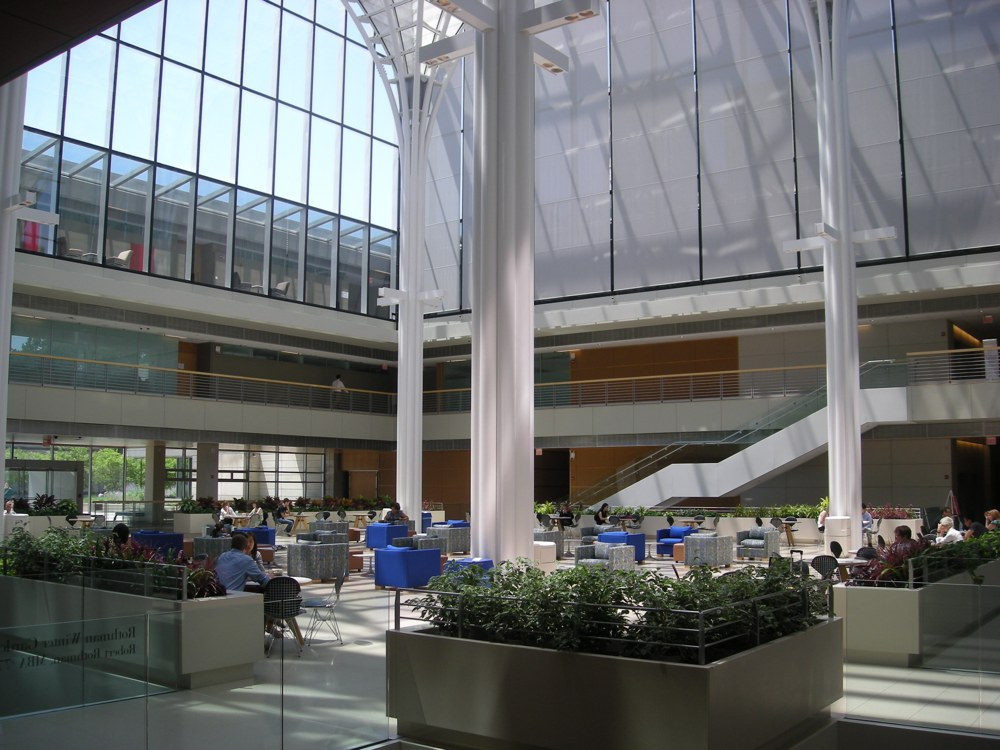
\includegraphics[height=0.36\textheight]{ch13_harper_center_2013.jpg}\\[1mm]
\imgcap{Charles M.\ Harper Center, Chicago Booth, where Gu and Xiu worked}
\imgcredit{https://commons.wikimedia.org/wiki/File:University_of_Chicago_July_2013_01_(Charles_M._Harper_Center).jpg}{Photo: Michael Barera (2013); CC BY-SA 4.0; Wikimedia Commons}
\end{column}
\end{columns}
\end{frame}

\begin{frame}{Evaluation in the Paper}
\itemsize{\small}
\begin{itemize}
    \item $R^2_{OOS} = 1 - \sum_{(i,t)}(r_{i,t+1} - \hat r_{i,t+1})^2 / \sum_{(i,t)} r_{i,t+1}^2$: the benchmark is a forecast of \textbf{zero}, not the historical mean
    \begin{itemize}
        \item $r_{i,t+1}$: the return of stock $i$ in month $t + 1$; $\hat r_{i,t+1}$: its forecast; the sums run over all stock-months of the test period
        \item the authors note that the historical mean of a stock is so noisy that it is easy to beat: a zero benchmark is harder
    \end{itemize}
    \item Diebold--Mariano tests between all pairs of models, with a Bonferroni correction for the 12 comparisons
    \begin{itemize}
        \item the same tool as Section 7, applied to a panel of stocks
    \end{itemize}
    \item Economic value: each month, sort stocks into deciles by forecast; buy the top decile, sell the bottom one
    \begin{itemize}
        \item value-weighted portfolios; Sharpe ratio, drawdown and turnover (the share of the portfolio traded each month)
    \end{itemize}
\end{itemize}
\end{frame}

\begin{frame}{Results: Small $R^2$, Large Economic Value}
\itemsize{\footnotesize}
\begin{center}
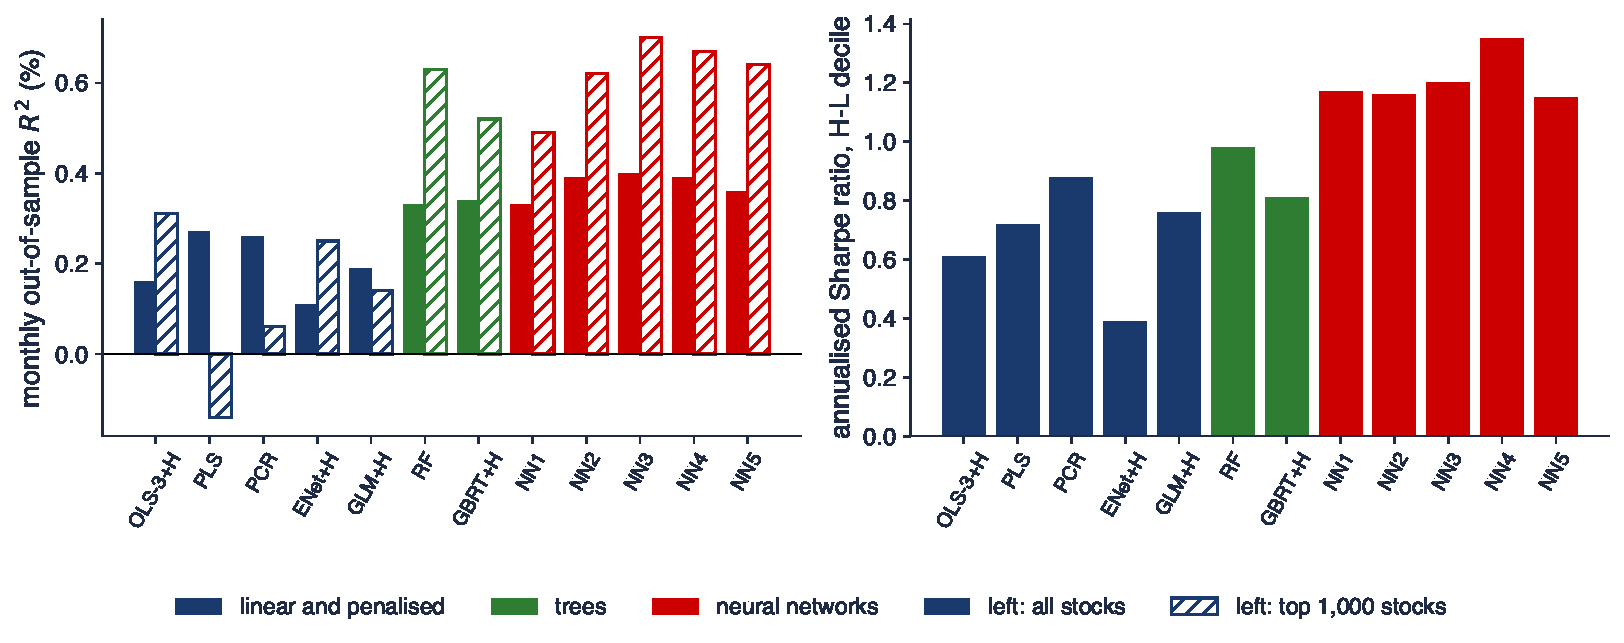
\includegraphics[width=0.97\textwidth,height=0.48\textheight,keepaspectratio]{sfm_ch13_gkx.pdf}
\end{center}
\vspace{-0.25cm}
\begin{itemize}
    \item Left: monthly $R^2_{OOS}$ (Table 1): OLS with all 920 features $-3.46\%$; OLS-3 (size, value, momentum) $0.16\%$; random forest $0.33\%$; NN3 $0.40\%$ ($0.70\%$ for the 1,000 largest stocks)
    \item Right: annual Sharpe ratio of the value-weighted decile spread (Table 7): OLS-3 $0.61$, random forest $0.98$, NN4 $1.35$
\end{itemize}
\sfmquantlet{Ch_13}{SFM_ch13_case_gkx}
\end{frame}

\begin{frame}{Interpretation and Limits}
\itemsize{\small}
\begin{itemize}
    \item What the paper shows
    \begin{itemize}
        \item nonlinear models (trees, networks) beat linear ones because they capture interactions between characteristics
        \item all methods agree on the main signals: price trends (momentum, short-term reversal), liquidity, volatility
        \item shallow networks are enough: 3--4 layers beat 5; ``deep'' learning does not help with monthly returns
    \end{itemize}
    \item What to keep in mind
    \begin{itemize}
        \item an $R^2_{OOS}$ below 1\% per month is a large result here: compare with the sign forecasts of Section 8
        \item neural portfolios turn over more than 100\% of their value each month: trading costs reduce the gains
        \item the evidence is a cross-section of thousands of stocks; it says little about timing one index
    \end{itemize}
\end{itemize}
\end{frame}


%=============================================================================
\section{AI for Scientific Discovery}
%=============================================================================

\begin{frame}{An Open Question}
\itemsize{\small}
\begin{itemize}
    \item \textbf{Do machine-learning volatility forecasts help on the Bucharest Stock Exchange, where liquidity is low and intraday data are scarce?}
    \begin{itemize}
        \item today: on the S\&P 500 the lasso gains $+7.1\%$ over HAR; on Bitcoin no significant gain ($+2.0\%$, p 0.520)
        \item the BET has no high and low prices in our data, so the proxy must come from squared returns, which are noisier
    \end{itemize}
    \item Why it is open: thin trading, a different calendar from New York, few crises in the sample
    \item Related work, as further reading: \refPeleA{} (statistical classification of crypto assets); \refPeleB{} (how precise forecast comparisons can be)
    \item AI tools can speed up such a study; they do not replace checking it \refWang
\end{itemize}
\end{frame}

\begin{frame}{How AI Could Help}
\itemsize{\small}
\begin{itemize}
    \item \textbf{Literature}: a list of studies on HAR and machine learning for emerging and frontier markets
    \item \textbf{Code}: a first draft of the walk-forward comparison of HAR, lasso and random forest for the BET and three BVB stocks
    \item \textbf{Robustness}: other proxies (absolute returns, two-day returns), other horizons (1, 5, 22 days), S\&P 500 features of the previous close
    \item Example prompt
    \begin{itemize}
        \item \aiprompt{Write Python code that compares HAR, lasso and a random forest for the weekly log variance of the BET index (proxy: squared daily returns), with yearly walk-forward refits from 2012, purging the last 5 training rows, and reports the out-of-sample R2, QLIKE and Diebold-Mariano tests.}
    \end{itemize}
\end{itemize}
\end{frame}

\begin{frame}{What to Check}
\itemsize{\small}
\begin{itemize}
    \item Time order: no shuffled folds; features use only data up to the close of day $t$; the last training targets do not reach into the test period
    \item Scaling and tuning inside the training window only (standardisation, $\lambda$, the number of trees)
    \item Calendars: the BVB closes before New York; S\&P 500 features must come from the previous New York close
    \item A benchmark in every table (HAR, the majority class, historical simulation) and a test of the difference
    \item The number of models tried, reported; references: every cited paper must exist; check the DOI
\end{itemize}
\end{frame}

\begin{frame}{Project Idea}
\itemsize{\small}
\begin{itemize}
    \item \textbf{Question}: do machine-learning models forecast the volatility of BVB stocks better than HAR?
    \begin{itemize}
        \item data: BET, Banca Transilvania, OMV Petrom, BRD (EODHD); S\&P 500 and DAX as external features
    \end{itemize}
    \item Steps
    \begin{itemize}
        \item a variance proxy for each stock (range where available, squared returns otherwise), weekly target
        \item HAR, lasso, random forest and a small MLP, walk-forward from 2014, yearly refits with purging
        \item out-of-sample $R^2$, QLIKE and Diebold--Mariano; Shapley values for the external features
    \end{itemize}
    \item Deliverable: one table, one chart, and a paragraph on what the data can and cannot show
    \item Declare any AI use, and list the errors of the AI that you corrected
\end{itemize}
\end{frame}


%=============================================================================
\section{Summary}
%=============================================================================

\begin{frame}{Key Takeaways}
\itemsize{\small}
\begin{itemize}
    \item Machine learning is judged by its error on new data; the bias--variance trade-off sets how flexible a model should be
    \item Time series need walk-forward validation with purging; random folds on overlapping targets fake predictability
    \item Ridge and lasso shrink; forests average trees; boosting adds trees; networks learn nonlinear features
    \item Volatility: HAR is hard to beat, the gains are a few per cent; the sign of returns: no gain over ``always up''
    \item VaR 1\%: linear quantile regression works; flexible quantile models lack tail data
    \item Report the number of trials and deflate the Sharpe ratio; compare every model with a simple benchmark
\end{itemize}
\end{frame}

\begin{frame}{Key Formulas}
\itemsize{\small}
{\renewcommand{\arraystretch}{1.45}\begin{center}
\scriptsize
\begin{tabular}{ll}
\toprule
\textbf{Quantity} & \textbf{Formula} \\
\midrule
Bias--variance & $E[(y_0 - \hat f)^2] = (E\hat f - f)^2 + \mathrm{Var}(\hat f) + \sigma^2$ \\
Ridge & $(X^\top X + \lambda I)^{-1}X^\top y$; \ 1D: $S_{xy}/(S_{xx} + \lambda)$ \\
Lasso (1D) & $\mathrm{sign}(S_{xy})\max(|S_{xy}| - \lambda/2, 0)/S_{xx}$ \\
Random forest & $\mathrm{Var} = \rho\sigma^2 + (1 - \rho)\sigma^2/B$ \\
Boosting & $F_m = F_{m-1} + \nu h_m$ \\
MLP & $\hat y = c + \sum_k v_k g(b_k + w_k^\top x)$ \\
HAR & $y_t = \beta_0 + \beta_d\ln v_t + \beta_w\ln v_t^{(w)} + \beta_m\ln v_t^{(m)} + u_t$ \\
$R^2_{OOS}$ & $1 - \sum(y - \hat y)^2/\sum(y - \tilde y)^2$ \\
Quantile loss & $\rho_\alpha(u) = u(\alpha - \mathbf{1}\{u < 0\})$ \\
DSR & $\Phi\big((\widehat{SR} - SR_0)\sqrt{T - 1}/\sqrt{1 - \hat\gamma_3\widehat{SR} + (\hat\gamma_4 - 1)\widehat{SR}^2/4}\big)$ \\
\bottomrule
\end{tabular}
\end{center}
}
\end{frame}

\begin{frame}{Check Yourself}
\itemsize{\small}
\begin{itemize}
    \item \textbf{Question}: a model has a training $R^2$ of 80\% and an out-of-sample $R^2$ of $-5\%$. What happened?
    \begin{itemize}
        \item \textbf{Answer}: overfitting: the model learned the noise of the training sample and loses against the benchmark on new data
    \end{itemize}
    \item \textbf{Question}: why is random K-fold wrong for a 21-day return target?
    \begin{itemize}
        \item \textbf{Answer}: neighbouring targets overlap, so the test answers leak into training; use walk-forward with purging
    \end{itemize}
    \item \textbf{Question}: a classifier is right on 53\% of the days and the market rose on 54\% of them. Is it useful?
    \begin{itemize}
        \item \textbf{Answer}: no: ``always up'' is right on 54\% of the days
    \end{itemize}
    \item Next: \sfmchlink{https://danpele.github.io/SFM/EN/Courses/chapter14_crypto_assets.pdf}{Chapter 14}, crypto assets
\end{itemize}
\end{frame}


%=============================================================================
\section{References}
%=============================================================================

\begin{frame}{References (1/3)}
\itemsize{\tiny}
\begin{itemize}
    \item Bailey, D.H., López de Prado, M. (2014). \href{https://doi.org/10.3905/jpm.2014.40.5.094}{The deflated Sharpe ratio: correcting for selection bias, backtest overfitting, and non-normality}. \textit{Journal of Portfolio Management}, 40(5), 94--107.
    \item Bergmeir, C., Hyndman, R.J., Koo, B. (2018). \href{https://doi.org/10.1016/j.csda.2017.11.003}{A note on the validity of cross-validation for evaluating autoregressive time series prediction}. \textit{Computational Statistics \& Data Analysis}, 120, 70--83.
    \item Breiman, L. (2001a). \href{https://doi.org/10.1214/ss/1009213726}{Statistical modeling: the two cultures}. \textit{Statistical Science}, 16(3), 199--231.
    \item Breiman, L. (2001b). \href{https://doi.org/10.1023/A:1010933404324}{Random forests}. \textit{Machine Learning}, 45(1), 5--32.
    \item Campbell, J.Y., Thompson, S.B. (2008). \href{https://doi.org/10.1093/rfs/hhm055}{Predicting excess stock returns out of sample: can anything beat the historical average?} \textit{Review of Financial Studies}, 21(4), 1509--1531.
    \item Christensen, K., Siggaard, M., Veliyev, B. (2023). \href{https://doi.org/10.1093/jjfinec/nbac020}{A machine learning approach to volatility forecasting}. \textit{Journal of Financial Econometrics}, 21(5), 1680--1727.
    \item Christoffersen, P.F. (1998). \href{https://doi.org/10.2307/2527341}{Evaluating interval forecasts}. \textit{International Economic Review}, 39(4), 841--862.
    \item Corsi, F. (2009). \href{https://doi.org/10.1093/jjfinec/nbp001}{A simple approximate long-memory model of realized volatility}. \textit{Journal of Financial Econometrics}, 7(2), 174--196.
    \item Diebold, F.X., Mariano, R.S. (1995). \href{https://doi.org/10.1080/07350015.1995.10524599}{Comparing predictive accuracy}. \textit{Journal of Business \& Economic Statistics}, 13(3), 253--263.
    \item Engle, R.F. (1982). \href{https://doi.org/10.2307/1912773}{Autoregressive conditional heteroscedasticity with estimates of the variance of United Kingdom inflation}. \textit{Econometrica}, 50(4), 987--1007.
    \item Engle, R.F., Manganelli, S. (2004). \href{https://doi.org/10.1198/073500104000000370}{CAViaR: conditional autoregressive value at risk by regression quantiles}. \textit{Journal of Business \& Economic Statistics}, 22(4), 367--381.
    \item Franke, J., Härdle, W.K., Hafner, C.M. (2019). \href{https://doi.org/10.1007/978-3-030-13751-9}{\textit{Statistics of Financial Markets: An Introduction}}, 5th ed. Springer.
\end{itemize}
\end{frame}

\begin{frame}{References (2/3)}
\itemsize{\tiny}
\begin{itemize}
    \item Friedman, J.H. (2001). \href{https://doi.org/10.1214/aos/1013203451}{Greedy function approximation: a gradient boosting machine}. \textit{Annals of Statistics}, 29(5), 1189--1232.
    \item Garman, M.B., Klass, M.J. (1980). \href{https://doi.org/10.1086/296072}{On the estimation of security price volatilities from historical data}. \textit{Journal of Business}, 53(1), 67--78.
    \item Gu, S., Kelly, B., Xiu, D. (2020). \href{https://doi.org/10.1093/rfs/hhaa009}{Empirical asset pricing via machine learning}. \textit{Review of Financial Studies}, 33(5), 2223--2273.
    \item Harvey, C.R., Liu, Y., Zhu, H. (2016). \href{https://doi.org/10.1093/rfs/hhv059}{\ldots and the cross-section of expected returns}. \textit{Review of Financial Studies}, 29(1), 5--68.
    \item Hastie, T., Tibshirani, R., Friedman, J. (2009). \href{https://doi.org/10.1007/978-0-387-84858-7}{\textit{The Elements of Statistical Learning}}, 2nd ed. Springer.
    \item Hoerl, A.E., Kennard, R.W. (1970). \href{https://doi.org/10.1080/00401706.1970.10488634}{Ridge regression: biased estimation for nonorthogonal problems}. \textit{Technometrics}, 12(1), 55--67.
    \item Hornik, K., Stinchcombe, M., White, H. (1989). \href{https://doi.org/10.1016/0893-6080(89)90020-8}{Multilayer feedforward networks are universal approximators}. \textit{Neural Networks}, 2(5), 359--366.
    \item James, G., Witten, D., Hastie, T., Tibshirani, R., Taylor, J. (2023). \href{https://doi.org/10.1007/978-3-031-38747-0}{\textit{An Introduction to Statistical Learning with Applications in Python}}. Springer.
    \item Kelly, B., Xiu, D. (2023). \href{https://doi.org/10.1561/0500000064}{Financial machine learning}. \textit{Foundations and Trends in Finance}, 13(3--4), 205--363.
    \item Koenker, R., Bassett, G. (1978). \href{https://doi.org/10.2307/1913643}{Regression quantiles}. \textit{Econometrica}, 46(1), 33--50.
    \item Kupiec, P.H. (1995). \href{https://doi.org/10.3905/jod.1995.407942}{Techniques for verifying the accuracy of risk measurement models}. \textit{Journal of Derivatives}, 3(2), 73--84.
    \item Lundberg, S.M., Lee, S.-I. (2017). \href{https://proceedings.neurips.cc/paper/2017/hash/8a20a8621978632d76c43dfd28b67767-Abstract.html}{A unified approach to interpreting model predictions}. \textit{Advances in Neural Information Processing Systems}, 30.
\end{itemize}
\end{frame}

\begin{frame}{References (3/3)}
\itemsize{\tiny}
\begin{itemize}
    \item López de Prado, M. (2018). \href{https://www.wiley.com/en-us/Advances+in+Financial+Machine+Learning-p-9781119482086}{\textit{Advances in Financial Machine Learning}}. Wiley.
    \item Patton, A.J. (2011). \href{https://doi.org/10.1016/j.jeconom.2010.03.034}{Volatility forecast comparison using imperfect volatility proxies}. \textit{Journal of Econometrics}, 160(1), 246--256.
    \item Pele, D.T., Mazurencu-Marinescu-Pele, M. (2026). \href{https://doi.org/10.3390/math14132316}{Finite-sample precision limits for expected shortfall forecast comparisons}. \textit{Mathematics}, 14(13), 2316.
    \item Pele, D.T., Wesselhöfft, N., Härdle, W.K., Kolossiatis, M., Yatracos, Y.G. (2023). \href{https://doi.org/10.1080/1351847X.2021.1960403}{Are cryptos becoming alternative assets?} \textit{European Journal of Finance}, 29(10), 1064--1105.
    \item Rosenblatt, F. (1958). \href{https://doi.org/10.1037/h0042519}{The perceptron: a probabilistic model for information storage and organization in the brain}. \textit{Psychological Review}, 65(6), 386--408.
    \item Rumelhart, D.E., Hinton, G.E., Williams, R.J. (1986). \href{https://doi.org/10.1038/323533a0}{Learning representations by back-propagating errors}. \textit{Nature}, 323, 533--536.
    \item Tibshirani, R. (1996). \href{https://doi.org/10.1111/j.2517-6161.1996.tb02080.x}{Regression shrinkage and selection via the lasso}. \textit{Journal of the Royal Statistical Society, Series B}, 58(1), 267--288.
    \item Wang, H., Fu, T., Du, Y., Gao, W., et al. (2023). \href{https://doi.org/10.1038/s41586-023-06221-2}{Scientific discovery in the age of artificial intelligence}. \textit{Nature}, 620, 47--60.
    \item Welch, I., Goyal, A. (2008). \href{https://doi.org/10.1093/rfs/hhm014}{A comprehensive look at the empirical performance of equity premium prediction}. \textit{Review of Financial Studies}, 21(4), 1455--1508.
    \item White, H. (2000). \href{https://doi.org/10.1111/1468-0262.00152}{A reality check for data snooping}. \textit{Econometrica}, 68(5), 1097--1126.
\end{itemize}
\end{frame}

\end{document}
